%!TEX root = main.tex

\section{Semantics of $A \xrightarrow{\finishstart(\phi)} B$ for {$\LMAOAMASS$}}\label{app-finishstart-lmaoamss}
In the sequel, assuming that $\Mm$ is an $\LMAOAMASS$.

Let $\rho = (\Omega_1,\cdots,\Omega_n)$ be a configuration with  $\Omega_i = (S_i, A_i, \zeta_i)$ for each $i\in[n]$, and $S=[B_1,\cdots,B_m]$ be a task. 
% Let $(\rho,b)$ be a configuration with $\rho = (\Omega_1,\cdots,\Omega_n)$ and $\Omega_i = (S_1,A_i,\zeta_i)$ for each $i\in[n]$, and $S=[B_1,\cdots,B_m]$ be a task. 
The following additional auxiliary function $\rmact(\rho,i, j)$ is defined for $\finishstart$.
\begin{itemize}
    \item let $1 \le i \le n$, $S_i = [C_1, \cdots, C_l]$ and $1 \le j \le l$, then $\rmact(\rho,i, j) = (\Omega_1,\cdots,\Omega_{i-1},(S_i',A_i,\zeta_i),\Omega_{i+1},\cdots,\Omega_n)$ if $l>1$, where $S_i' = [C_1,\cdots, C_{j-1}, C_{j+1},\cdots, C_l]$, and $\rmact(\rho,i, j) = (\Omega_1,\cdots,\Omega_{i-1},\Omega_{i+1},\cdots,\Omega_n)$ otherwise.
\end{itemize}

We present the semantics of the transition rules $A \xrightarrow{\finishstart(\phi)} B$.

\smallskip
\noindent \fbox{$\lmd(B) = \STD$}
	\begin{itemize}
		\item If $\lmd(A) \neq \SIT$, then $\rho'= \rmact(\push(\rho,B), 1, 2)$.
		%
		\item If $\lmd(A) = \SIT$, then
    		\begin{itemize}
                \item if $\getrealtsk(\rho,B) = S_i$ and $\zeta_i\neq\mainflag$, then $\rho'=\rmact(\mvtsktop(\rho, i), 2, 1)$,
                \item if $\getrealtsk(\rho,B) = S_i$ and $\zeta_i = \mainflag$, or $\getrealtsk(\rho,B) = *\wedge \gettsk(\rho,B) = S_i$, \\then $\rho'=\rmact(\push(\mvtsktop(\rho, i),B), 2, 1)$,
    			\item if $\gettsk(\rho, B)=*$, then $\rho'= \rmact(\newtsk(\rho, B, \STK), 2, 1)$.
    		\end{itemize}
	\end{itemize}

\noindent  \fbox{$\lmd(B) = \STP$}
	\begin{itemize}
		\item  If $\lmd(A) \neq \SIT$, then
        \begin{itemize}
            \item if $A = B$, then $\rho' = \rmact(\rho, 1, 1)$,
            \item otherwise, $\rho' = \rmact(\push(\rho, B), 1, 2)$.
        \end{itemize}
		%
		\item If $\lmd(A) = \SIT$, then
    		\begin{itemize}
                \item if $\getrealtsk(\rho,B) = S_i$ and $\zeta_i\neq\mainflag$, then $\rho'=\rmact(\mvtsktop(\rho, i), 2, 1)$,
                \item if $\getrealtsk(\rho,B) = S_i$ and $\zeta_i = \mainflag$, or $\getrealtsk(\rho,B) = *\wedge \gettsk(\rho,B) = S_i$, 
                \begin{itemize}
                    \item if $\topact(S_i) = B$, then $\rho' = \rmact(\mvacttop(\rho,i), 2, 1)$,
                    \item otherwise $\rho'=\rmact(\push(\mvtsktop(\rho, i),B), 2, 1)$,
                \end{itemize}
                % then $\rho'=\push(\mvtsktop(\rho, i),B)$,
    			\item if $\gettsk(\rho, B)=*$, then $\rho'= \rmact(\newtsk(\rho,B, \STK), 2, 1)$.
    		\end{itemize}
	 \end{itemize}
	
\noindent \fbox{$\lmd(B) = \SIT$}
\begin{itemize}
	\item If $\getrealtsk(\rho, B) = S_1$, then $\rho' = \rmact(\rho, 1, 1)$.
	\item If $\getrealtsk(\rho, B) = S_i$ and $i > 1$, then $\rho' = \rmact(\mvtsktop(\rho, i), 2, 1)$.
	\item If $\getrealtsk(\rho, B) = *$, then $\rho' = \rmact(\newtsk(\rho, B,\SIT), 2, 1)$.
\end{itemize}

\noindent  \fbox{$\lmd(B) = \singletask$}
\begin{itemize}
	\item If $\getrealtsk(\rho, B) = S_i$, or $\getrealtsk(\rho,B) = *\wedge\gettsk(\rho,B) = S_i$ then
	\begin{itemize}
		\item if $i = 1$,
		\begin{itemize}
			\item if $B \not \in S_i$, then $\rho' = \rmact(\push(\rho, B), 1, 2)$,
			\item if $B \in S_i$, 
			\begin{itemize}
				\item if $\topact(\rho) = B$, then $\rho' = \rmact(\rho, 1, 1)$,
				\item if $\topact(\rho) \neq B$, then $\rho' = \clrtop(\rho, B)$,
			\end{itemize}
		\end{itemize}
		\item if $i > 1$,
		\begin{itemize}
			\item if $B \not \in S_i$, then $\rho' = \rmact(\push(\mvtsktop(\rho, i), B), 2, 1)$,
			\item if $B \in S_i$, 	then $\rho' =  \rmact(\clrtop(\mvtsktop(\rho, i), B), 2, 1)$.
		\end{itemize}
	\end{itemize}
\item If $\gettsk(\rho, B) = *$, then $\rho' = \rmact(\newtsk(\rho, B,\STK), 2, 1)$.
\end{itemize}

\section{Semantics of {$\IFAOAMASS$}}\label{app-ifaoamass}

In the sequel, assuming that $\Mm$ is an $\IFAOAMASS$.
% we present the semantics of the transition rules $A \xrightarrow{\finishstart(\phi)} B$.
Firstly, we need adapt the concept of configurations as follows:
A configuration of $\Mm$ is 
% still encoded as a sequence
encoded as a pair $(\rho, b)$, where $b \in \{\nohflag, \neg \nohflag\}$ and 
$\rho=(\Omega_1,\cdots,\Omega_n)$ such that for each $i \in [n]$, $\Omega_i = (S_i, A_i, \zeta_i)$, where $S_i \in \act^*$ is a task, $A_i \in \act$ is the real activity of $S_i$, but $\zeta_i \in \{\mainflag, \ntkflag, \ndmflag\}$. Intuitively, 
% $b$ denotes whether the topmost activity is started with $\nohflag$ or not, 
$\ntkflag$ in $\zeta_i$ plays the same role as $\STK$ in $\LMAOAMASS$, and $\ndmflag$ is added for the intent flag $\ndmflag$, moreover, $\SIT$ disappears since in $\IFAOAMASS$, the launch modes of all activities are assumed to be $\STD$.
% A configuration of $\Mm$ is encoded as a pair $(\rho, b)$, where $b \in \{\nohflag, \neg \nohflag\}$. Intuitively, $b$ denotes whether the topmost activity is started with $\nohflag$ or not.

Let us define the semantics of $\Mm$ by a relation 
% $\rho \xrightarrow[\Mm]{\startactivity(\phi)} \rho'$ with $\phi \models \neg \tohflag \wedge \neg \nohflag$.
$\rho \xrightarrow[\tau]{\Mm} \rho'$ with $\tau = A \xrightarrow{\alpha(\phi)} B$.
Let us consider the subcase $\phi \models \neg \tohflag$ first.

\smallskip
\noindent \fbox{$\phi \models \neg \ntkflag\wedge\neg\ndmflag$}
	\begin{itemize}
		\item If $\phi \models \ctpflag$ and $B \in \toptsk(\rho)$, then 
		\begin{itemize}
			\item if $\topact(\rho) \neq B$, then $\rho' = \clrtop(\rho, B)$, moreover, 
			\begin{itemize}
			\item if $\phi \models \neg \stpflag$, then $b' = \nohflag$ iff $\phi \models \nohflag$, 
			\item otherwise, $b' = \neg \nohflag$,
			\end{itemize}
			\item if $\topact(\rho) = B$, 
			\begin{itemize}
					\item if $\phi \models \stpflag$, then
					\begin{itemize}
						\item if $\alpha = \startactivity$, then $\rho' = \rho$ and $b' = b$,
						\item if $\alpha = \finishstart$, then $\rho' = \rmact(\rho, 1, 1)$ and $b' = \neg \nohflag$,
					\end{itemize}
					\item if $\phi \models \neg \stpflag$, then $\rho' = \rho$ and $b' = \nohflag$ iff $\phi \models \nohflag$.
				% \item if $\alpha = \startactivity$, then $\rho' = \rho$,
				% \item if $\alpha = \startactivity$, then $\rho' = \rho$, moreover, 
				% \begin{itemize}
				% 	\item if $\phi \models \neg \stpflag$, then 
				% 	$b' = \nohflag$ iff $\phi \models \nohflag$, 
				% 	\item otherwise, $b' = b$,
				% \end{itemize}
				% \item if $\alpha = \finishstart$, then $\rho' = \rmact(\rho, 1, 1)$ and $b' = \nohflag$ iff $\phi \models \nohflag$, 
			% \end{itemize}
			% \end{itemize}
			% $\rho' = \rho$, moreover,
		\end{itemize}
		\end{itemize}
		\item If $\phi \models \ctpflag$ and $B \notin \toptsk(\rho)$, then $b' = \nohflag$ iff $\phi \models \nohflag$, moreover,
		\begin{itemize}
			\item if $b = \neg \nohflag$ and $\alpha = \startactivity$, then $\rho' = \push(\rho, B)$, 
			\item otherwise, $\rho' = \rmact( \push(\rho, B), 1, 2)$. 
		\end{itemize}
		\item If $\phi \models \neg \ctpflag$, then
		\begin{itemize}
			\item if $\phi \models \rtfflag$ and $B \in \toptsk(\rho)$, then
			\begin{itemize}
				\item if $\topact(\rho) \neq B$, then $b' = \neg \nohflag$, moreover, 
				\begin{itemize}
					\item if $b = \neg \nohflag$ and $\alpha = \startactivity$, then $\rho'= \mvacttop(\rho, B)$, 
					\item otherwise, $\rho' = \rmact(\mvacttop(\rho, B), 1, 2)$, 
				\end{itemize}
				\item if $\topact(\rho) = B$, 
				\begin{itemize}
					\item if $\alpha = \startactivity$, then $\rho' = \rho$ and $b' = b$,
					\item if $\alpha = \finishstart$, then $\rho = \rmact(\rho, 1, 1)$, and $b' = \neg \nohflag$,
				\end{itemize}
			\end{itemize}
			\item if $\phi \models \rtfflag$ and $B \notin \toptsk(\rho)$, then $b' = \nohflag$ iff $\phi \models \nohflag$, moreover,
			\begin{itemize}
				\item if $b = \neg \nohflag$ and $\alpha = \startactivity$, then $\rho' = \push(\rho, B)$, 
				\item otherwise, $\rho' = \rmact( \push(\rho, B), 1, 2)$. 
			\end{itemize}
			\item If $\phi \models \neg \rtfflag$, then
			\begin{itemize}
				\item if $\phi \models \stpflag$ and $\topact(\rho) = B$ or $\phi \models \stpflag\wedge\pitflag$ and $\preact(\rho) = B$, 
				\begin{itemize}
					\item if $\alpha = \startactivity$, then $\rho' = \rho$ and $b' = b$,
					\item if $\alpha = \finishstart$, then $\rho' = \rmact(\rho, 1, 1)$ and $b' = \neg \nohflag$,
				\end{itemize}
				\item otherwise, $b' = \nohflag$ iff $\phi \models \nohflag$, moreover,
				\begin{itemize}
					\item if $b = \neg \nohflag$ and $\alpha = \startactivity$, then $\rho' = \push(\rho, B)$, 
					\item otherwise, $\rho' = \rmact( \push(\rho, B), 1, 2)$. 
				\end{itemize}
			\end{itemize}
		\end{itemize}
\end{itemize}

\smallskip
\noindent \fbox{$\phi \models \ndmflag$}

\begin{itemize}
    \item If $\phi \models \mtkflag$, then $b' = \nohflag$ iff $\phi  \models \nohflag$, 
    \begin{itemize}
    	\item if $b = \neg \nohflag$ and $\alpha = \startactivity$, then $\rho'=\newtsk(\rho, B, \ndmflag)$, 
	\item otherwise, $\rho'= \rmact(\newtsk(\rho, B, \ndmflag), 2, 1)$.
    \end{itemize}
    %
    \item If $\phi \models \neg \mtkflag$, then
   \begin{itemize}
        \item if $\getrealtsk(\rho, B) = S_i$, then
	\begin{itemize}
		\item if $i \neq 1$, then
        			\begin{itemize}
            			\item if $\phi \models \neg \ctkflag$, then 
				\begin{itemize}
					\item if $B \not \in S_i$, then $b' = \nohflag$ iff $\phi  \models \nohflag$, moreover, 
					\begin{itemize}
						\item if $b = \neg \nohflag$ and $\alpha = \startactivity$, then $\rho' = \push(\mvtsktop(\rho, i), B)$, 
						\item otherwise, $\rho' = \rmact(\push(\mvtsktop(\rho, i), B), 2, 1)$, 
					\end{itemize}
					\item otherwise, $b' = \neg \nohflag$,
					% \begin{itemize}
					% 	\item if $\phi \models \neg \stpflag$, then $b' = \nohflag$ iff $\phi  \models \nohflag$, 
					% 	\item otherwise, $b' = \neg \nohflag$, 
					% \end{itemize}
					moreover, 
					\begin{itemize}
						\item if $b = \neg \nohflag$ and $\alpha = \startactivity$, then $\rho'=\clrtop(\mvtsktop(\rho, i), B)$, 
						\item otherwise,  $\rho'= \rmact(\clrtop(\mvtsktop(\rho, i), B), 2, 1)$, 
					\end{itemize}
				\end{itemize}
            			\item if $\phi \models \ctkflag$, then $b' = \nohflag$ iff $\phi  \models \nohflag$, moreover, 
				\begin{itemize}
						\item if $b = \neg \nohflag$ and $\alpha = \startactivity$, then $\rho'=\clrtsk(\mvtsktop(\rho, i), B)$, 
						\item otherwise,  $\rho'= \rmact(\clrtsk(\mvtsktop(\rho, i), B), 2, 1)$, 
				\end{itemize}
        			\end{itemize}
		\item otherwise ($i = 1$), 
        			\begin{itemize}
            			\item if $\phi \models \neg \ctkflag$, then 
            			\begin{itemize}
					\item if $B \not \in S_1$, then $b' = \nohflag$ iff $\phi  \models \nohflag$, moreover, 
					\begin{itemize}
						\item if $b = \neg \nohflag$ and $\alpha = \startactivity$, then $\rho'=\push(\rho, B)$,
						\item otherwise, $\rho' = \rmact(\push(\rho, B), 1, 2)$,  
					\end{itemize}
            				\item if $B \in S_1$ and $\topact(S_1) \neq B$, then $\rho'= \clrtop(\rho, B)$ and $b' = \neg\nohflag$,
					% \begin{itemize}
					% 	\item if $\phi \models \stpflag$, then $b' = \neg \nohflag$, 
					% 	\item otherwise, $b' = \nohflag$ iff $\phi  \models \nohflag$,
					% \end{itemize}
					\item if $B \in S_1$ and $\topact(S_1) = B$ (this implies $A = B$), then 
					\begin{itemize}
						\item if $\alpha = \startactivity$, then $\rho' = \rho$ and $b' = b$,
						\item if $\alpha = \finishstart$, then $\rho' = \rmact(\rho, 1, 1)$ and $b' = \neg \nohflag$,
					\end{itemize}
			 	\end{itemize}
            			\item if $\phi \models \ctkflag$, then $\rho'= \clrtsk(\rho, B)$, and $b' = \nohflag$ iff $\phi  \models \nohflag$, 
				% \begin{itemize}
				% 	\item if $\phi \models \stpflag$, then $b' = \neg \nohflag$, moreover, 
				% 	\begin{itemize}
				% 		\item if $B \not \in S_1$, then 
				% 	\end{itemize}
				% 	\item otherwise, $b' = \nohflag$	iff $\phi  \models \nohflag$, 		
				% \end{itemize}
            	% 		\begin{itemize}
				% 	\item if $B \not \in S_1$, then $b' = \nohflag$ iff $\phi  \models \nohflag$, moreover, 
				% 	\begin{itemize}
				% 		\item if $b = \neg \nohflag$, then $\rho' = \push(\rho, B)$,
				% 		\item otherwise, $\rho' = \rmact(\push(\rho, B), 1, 2)$, 
				% 	\end{itemize}
            	% 			\item if $B \in S_1$ and $\topact(S_1) \neq B$, then $\rho'= \clrtsk(\rho, B)$, moreover, $b' = \nohflag$ iff $\phi  \models \nohflag$, 
				% 	\item if $B \in S_1$ and $\topact(S_1) = B$ (this implies $A = B$), then $\rho'= \rho$ and $b' = b$,
			 	% \end{itemize}
        			\end{itemize}
	\end{itemize}
        \item if $\getrealtsk(\rho,B) = *$, then $b' = \nohflag$ iff $\phi \models \nohflag$, moreover,
        \begin{itemize}
        		\item if $b = \neg \nohflag$ and $\alpha = \startactivity$, then $\rho'=\newtsk(\rho, B, \ndmflag)$, 
		\item otherwise, $\rho'=\rmact(\newtsk(\rho, B, \ndmflag), 2, 1)$.
        \end{itemize}
    \end{itemize}
\end{itemize}    

\smallskip
\noindent \fbox{$\phi \models \ntkflag \wedge \neg \ndmflag$}

\begin{itemize}
\item If $\phi \models \mtkflag$,  then $b' = \nohflag$ iff $\phi \models \nohflag$, moreover, 
	\begin{itemize}
		\item if $b = \neg \nohflag$ and $\alpha = \startactivity$, then $\rho' = \newtsk(\rho, B, \ntkflag)$, 
		\item otherwise, $\rho' = \rmact(\newtsk(\rho, B, \ntkflag), 2, 1)$.
	\end{itemize}
%
\item If $\phi \models \neg \mtkflag$,  then
	\begin{itemize}
        \item if $\getrealtsk(\rho, B) = S_i$ or $\getrealtsk(\rho,B) = * \wedge\gettsk(\rho,B) = S_i$, then
        \begin{itemize}
        \item if $i \neq 1$, then 
			\begin{itemize}
				\item if $\phi \models \ctkflag$, then $b' = \nohflag$ iff $\phi \models \nohflag$, moreover, 
                \begin{itemize}
					\item if $b = \neg \nohflag$ and $\alpha = \startactivity$, then $\rho'=\clrtsk(\mvtsktop(\rho, i), B)$,
					\item otherwise, $\rho' = \rmact(\clrtsk(\mvtsktop(\rho, i), B), 2, 1)$, 
                \end{itemize}
				\item if $\phi \models \neg \ctkflag$, then
					\begin{itemize}
						\item if $\phi \models\ctpflag$ and $B \in S_i$, then 
						\begin{itemize}
							\item if $b = \neg \nohflag$ and $\alpha = \startactivity$, then $\rho'=\clrtop(\mvtsktop(\rho, i), B)$,
							\item otherwise, $\rho' = \rmact(\clrtop(\mvtsktop(\rho, i), B), 2, 1)$, 
						\end{itemize}
						moreover, 
						\begin{itemize}
							\item if $\phi\models \neg \stpflag$, then $b' = \nohflag$ iff $\phi \models \nohflag$, 
							\item otherwise $b' = \neg \nohflag$, 
						\end{itemize}
						\item if $\phi \models\ctpflag$ and $B \notin S_i$, then $b' = \nohflag$ iff $\phi \models \nohflag$, moreover, 
						\begin{itemize}
							\item if $b = \neg \nohflag$ and $\alpha = \startactivity$, then $\rho'=\push(\mvtsktop(\rho, i), B)$,
							\item otherwise, $\rho' = \rmact(\push(\mvtsktop(\rho, i), B), 2, 1)$, 
						\end{itemize}
						\item if $\phi \models\neg\ctpflag$, then
						\begin{itemize}
							\item if $\phi \models \rtfflag$ and $B\in S_i$, then $b' = \neg \nohflag$, moreover,
							\begin{itemize}
								\item if $b = \neg \nohflag$ and $\alpha = \startactivity$, then $\rho'=\mvacttop(\mvtsktop(\rho, i), B)$,
								\item otherwise, $\rho' = \rmact(\mvacttop(\mvtsktop(\rho, i), B), 2, 1)$, 
							\end{itemize}
							\item if $\phi \models \rtfflag$ and $B\notin S_i$, then $b' = \nohflag$ iff $\phi \models \nohflag$, moreover, 
							\begin{itemize}
								\item if $b = \neg \nohflag$ and $\alpha = \startactivity$, then $\rho'=\push(\mvtsktop(\rho, i), B)$,
								\item otherwise, $\rho' = \rmact(\push(\mvtsktop(\rho, i), B), 2, 1)$, 
							\end{itemize}
							\item if $\phi \models \neg \rtfflag$, then
							\begin{itemize}
								\item if $\getrealtsk(\rho,B) = S_i$ and $\zeta_i \neq \mainflag$, then $b' = \neg \nohflag$, moreover,
								\begin{itemize}
									\item if $b = \neg \nohflag$ and $\alpha = \startactivity$, then $\rho'=\mvtsktop(\rho, i)$,
									\item otherwise, $\rho' = \rmact(\mvtsktop(\rho, i), 2, 1)$, 
								\end{itemize}
								\item otherwise ($\getrealtsk(\rho,B) = S_i$ and $\zeta_i = \mainflag$ or $\getrealtsk(\rho,B) = * \wedge\gettsk(\rho,B) = S_i$), 
								\begin{itemize}
									\item if $\phi\models\stpflag$ and $\topact(S_i) = B$, then $b' = \neg \nohflag$, moreover,
									\begin{itemize}
										\item if $b = \neg \nohflag$ and $\alpha = \startactivity$, then $\rho'=\mvtsktop(\rho, i)$,
										\item otherwise, $\rho' = \rmact(\mvtsktop(\rho, i), 2, 1)$, 
									\end{itemize}
									\item otherwise, $b' = \nohflag$ iff $\phi \models \nohflag$, moreover, 
									\begin{itemize}
										\item if $b = \neg \nohflag$ and $\alpha = \startactivity$, then $\rho'=\push(\mvtsktop(\rho, i), B)$,
										\item otherwise, $\rho' = \rmact(\push(\mvtsktop(\rho, i), B), 2, 1)$, 
									\end{itemize}
								\end{itemize}
							\end{itemize}
						\end{itemize}
					\end{itemize}
			\end{itemize}
		\item otherwise ($i  = 1$),  
		\begin{itemize}
			\item if $\phi \models \ctkflag$, then $\rho' = \clrtsk(\rho,B)$ and $b' = \nohflag$ iff $\phi \models \nohflag$, 
			\item if $\phi \models \neg \ctkflag$, then
			\begin{itemize}
				\item if $\phi \models \ctpflag$ and $B \in S_1$, then $\rho'=\clrtop(\rho, B)$, moreover, 
%				\begin{itemize}
%					\item if $\phi\models \neg \stpflag$, then $b' = \nohflag$ iff $\phi \models \nohflag$, 
%					\item otherwise, $b' = \neg \nohflag$,
%				\end{itemize}
				\begin{itemize}
            				\item if $A \neq B$, then $\rho'=\clrtop(\rho, B)$, moreover, 
					\begin{itemize}
						\item if $\phi\models \neg \stpflag$, then $b' = \nohflag$ iff $\phi \models \nohflag$, 
						\item otherwise, $b' = \neg \nohflag$, 
					\end{itemize}
					\item if $A = B$, 
					% then $\rho' = \rho$, moroever,  
					\begin{itemize}
						\item if $\phi \models \stpflag$, then
						\begin{itemize}
							\item if $\alpha = \startactivity$, then $\rho' = \rho$ and $b' = b$,
							\item if $\alpha = \finishstart$, then $\rho' = \rmact(\rho, 1, 1)$ and $b' = \neg \nohflag$,
						\end{itemize}
						\item if $\phi \models \neg \stpflag$, then $\rho' = \rho$ and $b' = \nohflag$ iff $\phi \models \nohflag$,
						% \item if $\phi \models \neg \stpflag$, then $\rho' = \clrtop(\rho, B)$ and $b' = \nohflag$ iff $\phi \models \nohflag$, 
						% \item otherwise, $\rho' = \rho$ and $b' = b$,
					\end{itemize}
				\end{itemize}
				\item if $\phi \models \ctpflag$ and $B\notin S_1$, then $b' = \nohflag$ iff $\phi \models \nohflag$, moreover,
				\begin{itemize}
					\item if $b = \neg \nohflag$ and $\alpha = \startactivity$, then $\rho'=\push(\rho, B)$,
					\item otherwise, $\rho' = \rmact(\push(\rho, B), 1, 2)$, 
				\end{itemize}
				\item if $\phi \models \neg \ctpflag$, then
				\begin{itemize}
					\item if $\phi \models \rtfflag$ and $B \in S_1$, then
					\begin{itemize}
                					\item if $A \neq B$, then $b' = \neg \nohflag$, moreover, 
                					\begin{itemize}
                						\item if $b = \neg \nohflag$ and $\alpha = \startactivity$, then $\rho'=\mvacttop(\rho, B)$,
							\item otherwise, $\rho' = \rmact(\mvacttop(\rho, B), 1, 2)$,
						\end{itemize}
                					\item if $A = B$, 
									\begin{itemize}
										\item if $\alpha = \startactivity$, then $\rho' = \rho$ and $b' = b$, 
										\item if $\alpha = \finishstart$, then $\rho' = \rmact(\rho, 1, 1)$ and $b' = \neg \nohflag$, 
									\end{itemize}
                				\end{itemize}
					\item if $\phi \models \rtfflag$ and $B \notin S_1$, then $b' = \nohflag$ iff $\phi \models \nohflag$, moreover,
					\begin{itemize}
						\item if $b = \neg \nohflag$ and $\alpha = \startactivity$, then $\rho'=\push(\rho, B)$,
						\item otherwise, $\rho' = \rmact(\push(\rho, B), 1, 2)$, 
					\end{itemize}
					\item if $\phi \models \neg \rtfflag$, then
					\begin{itemize}
						\item if $\getrealtsk(\rho,B) = S_1$ and $\zeta_1 \neq \mainflag$, then 
						\begin{itemize}
							\item if $\alpha = \startactivity$, then $\rho' = \rho$ and $b' = b$,
							\item if $\alpha = \finishstart$, then $\rho' = \rmact(\rho, 1, 1)$ and $b' = \neg \nohflag$,
						\end{itemize}
						\item otherwise ($\getrealtsk(\rho,B) = S_1$ and $\zeta_i = \mainflag$ or $\getrealtsk(\rho,B) = * \wedge\gettsk(\rho,B) = S_1$), 
						\begin{itemize}
							\item if $\phi\models\stpflag$ and $A = B$, or $\phi \models\stpflag\wedge\pitflag$ and $\preact(\rho) = B$, 
							\begin{itemize}
								\item if $\alpha = \startactivity$, then $\rho' = \rho$ and $b' = b$,
								\item if $\alpha = \finishstart$, then $\rho' = \rmact(\rho, 1, 1)$ and $b' = \neg \nohflag$,
							\end{itemize}
							% then $\rho' = \rho$ and $b' = b$, 
							\item otherwise, $b' = \nohflag$ iff $\phi \models \nohflag$, moreover, 
							\begin{itemize}
								\item if $b = \neg \nohflag$ and $\alpha = \startactivity$, then $\rho'=\push(\rho, B)$,
								\item otherwise, $\rho' = \rmact(\push(\rho, B), 1, 2)$, 
							\end{itemize}
						\end{itemize}
					\end{itemize}
				\end{itemize}
			\end{itemize}
		\end{itemize}
	\end{itemize}
	    %
	\item if $\gettsk(\rho, B) = *$, then $b' = \nohflag$ iff $\phi \models \nohflag$, moreover, 
		\begin{itemize}
			\item if $b = \neg \nohflag$ and $\alpha = \startactivity$, then $\rho' = \newtsk(\rho, B, \ntkflag)$, 
			\item otherwise, $\rho' = \rmact(\newtsk(\rho, B, \ntkflag), 2, 1)$.
		\end{itemize}				
	\end{itemize}
\end{itemize}

Next, let us consider the subcase $\phi \models \tohflag$.
Let $\phi'$ be obtained from $\phi$ by replacing $\tohflag$ with $\neg \tohflag$. Moreover, 
suppose $\rho \xrightarrow [\tau']{\Mm} \rho'$, where $\tau' = A \xrightarrow{\alpha(\phi')} B$ and $\rho' = (\Omega_1, \cdots, \Omega_{n})$. 
% suppose $(\rho, b) \xrightarrow [\startactivity(\phi')]{\Mm} (\rho', b')$, where $\rho' = (\Omega_1, \cdots, \Omega_{n})$. 
\begin{itemize}
\item If $\phi \models \ntkflag \vee \ndmflag$, then let $\rho'' = (\Omega_1)$ and we have $\rho \xrightarrow [\tau]{\Mm} \rho''$.
%
\item Otherwise, $\rho \xrightarrow [\tau]{\Mm} \rho'$.
\end{itemize}

\hide{
Then we present the semantics of the transition rules $A \xrightarrow{\finishstart(\phi)} B$.

\smallskip
\noindent \fbox{$\phi \models \neg \ntkflag\wedge\neg\ndmflag$}
	\begin{itemize}
		\item If $\phi \models \ctpflag$ and $B \in \toptsk(\rho)$, then 
		\begin{itemize}
			\item if $\topact(\rho) \neq B$, then $\rho' = \clrtop(\rho, B)$, moreover, 
			\begin{itemize}
			\item if $\phi \models \neg \stpflag$, then $b' = \nohflag$ iff $\phi \models \nohflag$, 
			\item otherwise, $b' = \neg \nohflag$,
			\end{itemize}
			\item if $\topact(\rho) = B$, then 
			% $\rho' = \rmact(\rho,1,1)$, moreover,
			\begin{itemize}
				\item if $\phi \models \neg \stpflag$, then $\rho' =\rho$, and $b' = \nohflag$ iff $\phi \models \nohflag$, 
			   \item otherwise, $\rho' = \rmact(\rho, 1, 1)$ and $b' = \neg \nohflag$.
		   \end{itemize}
		\end{itemize}
		\item If $\phi \models \ctpflag$ and $B \notin \toptsk(\rho)$, then 
		$\rho' = \rmact( \push(\rho, B), 1, 2)$, and $b' = \nohflag$ iff $\phi \models \nohflag$.
		% \begin{itemize}
		% 	\item if $b = \neg \nohflag$, then $\rho' = \push(\rho, B)$, 
		% 	\item otherwise, $\rho' = \rmact( \push(\rho, B), 1, 2)$. 
		% \end{itemize}
		\item If $\phi \models \neg \ctpflag$, then
		\begin{itemize}
			\item if $\phi \models \rtfflag$ and $B \in \toptsk(\rho)$, then
			\begin{itemize}
				\item if $\topact(\rho) \neq B$, then $\rho' = \rmact(\mvacttop(\rho, B), 1, 2)$ and $b' = \neg \nohflag$,
				% \begin{itemize}
				% 	\item if $b = \neg \nohflag$, then $\rho'= \mvacttop(\rho, B)$, 
				% 	\item otherwise, $\rho' = \rmact(\mvacttop(\rho, B), 1, 2)$, 
				% \end{itemize}
				\item if $\topact(\rho) = B$, then $\rho' = \rmact(\rho, 1, 1)$ and $b' = \neg \nohflag$,
			\end{itemize}
			\item if $\phi \models \rtfflag$ and $B \notin \toptsk(\rho)$, then $\rho' = \rmact( \push(\rho, B), 1, 2)$, and $b' = \nohflag$ iff $\phi \models \nohflag$, 
			% \begin{itemize}
			% 	\item if $b = \neg \nohflag$, then $\rho' = \push(\rho, B)$, 
			% 	\item otherwise, $\rho' = \rmact( \push(\rho, B), 1, 2)$. 
			% \end{itemize}
			\item If $\phi \models \neg \rtfflag$, then
			\begin{itemize}
				\item if $\phi \models \stpflag$ and $\topact(\rho) = B$ or $\phi \models \stpflag\wedge\pitflag$ and $\preact(\rho) = B$, then $\rho' = \rmact(\rho, 1, 1)$ and $b' = \neg \nohflag$,
				\item otherwise, $\rho' = \rmact( \push(\rho, B), 1, 2)$, and $b' = \nohflag$ iff $\phi \models \nohflag$.
				% \begin{itemize}
				% 	\item if $b = \neg \nohflag$, then $\rho' = \push(\rho, B)$, 
				% 	\item otherwise, $\rho' = \rmact( \push(\rho, B), 1, 2)$. 
				% \end{itemize}
			\end{itemize}
		\end{itemize}
\end{itemize}

\smallskip
\noindent \fbox{$\phi \models \ndmflag$}

\begin{itemize}
    \item If $\phi \models \mtkflag$, then $\rho'= \rmact(\newtsk(\rho, B, \ndmflag), 2, 1)$, moreover, $b' = \nohflag$ iff $\phi  \models \nohflag$.
    % \begin{itemize}
    % 	\item if $b = \neg \nohflag$, then $\rho'=\newtsk(\rho, B, \ndmflag)$, 
	% \item otherwise, $\rho'= \rmact(\newtsk(\rho, B, \ndmflag), 2, 1)$.
    % \end{itemize}
    %
    \item If $\phi \models \neg \mtkflag$, then
   \begin{itemize}
        \item if $\getrealtsk(\rho, B) = S_i$, then
	\begin{itemize}
		\item if $i \neq 1$, then
        			\begin{itemize}
            			\item if $\phi \models \neg \ctkflag$, then 
				\begin{itemize}
					\item if $B \not \in S_i$, then $\rho' = \rmact(\push(\mvtsktop(\rho, i), B), 2, 1)$, and $b' = \nohflag$ iff $\phi  \models \nohflag$, 
					% \begin{itemize}
					% 	\item if $b = \neg \nohflag$, then $\rho' = \push(\mvtsktop(\rho, i), B)$, 
					% 	\item otherwise, $\rho' = \rmact(\push(\mvtsktop(\rho, i), B), 2, 1)$, 
					% \end{itemize}
					\item otherwise, $\rho'= \rmact(\clrtop(\mvtsktop(\rho, i), B), 2, 1)$ and $b' = \neg \nohflag$,
					% \begin{itemize}
					% 	\item if $\phi \models \neg \stpflag$, then $b' = \nohflag$ iff $\phi  \models \nohflag$, 
					% 	\item otherwise, $b' = \neg \nohflag$, 
					% \end{itemize}
					% moreover, 
					% \begin{itemize}
					% 	\item if $b = \neg \nohflag$, then $\rho'=\clrtop(\mvtsktop(\rho, i), B)$, 
					% 	\item otherwise,  $\rho'= \rmact(\clrtop(\mvtsktop(\rho, i), B), 2, 1)$, 
					% \end{itemize}
				\end{itemize}
            			\item if $\phi \models \ctkflag$, then $\rho'= \rmact(\clrtsk(\mvtsktop(\rho, i), B), 2, 1)$, and $b' = \nohflag$ iff $\phi  \models \nohflag$, 
				% \begin{itemize}
				% 		\item if $b = \neg \nohflag$, then $\rho'=\clrtsk(\mvtsktop(\rho, i), B)$, 
				% 		\item otherwise,  $\rho'= \rmact(\clrtsk(\mvtsktop(\rho, i), B), 2, 1)$, 
				% \end{itemize}
        			\end{itemize}
		\item otherwise ($i = 1$), 
        			\begin{itemize}
            			\item if $\phi \models \neg \ctkflag$, then 
            			\begin{itemize}
					\item if $B \not \in S_1$, then $\rho' = \rmact(\push(\rho, B), 1, 2)$, and $b' = \nohflag$ iff $\phi  \models \nohflag$, 
					% \begin{itemize}
					% 	\item if $b = \neg \nohflag$, then $\rho'=\push(\rho, B)$,
					% 	\item otherwise, $\rho' = \rmact(\push(\rho, B), 1, 2)$,  
					% \end{itemize}
            				\item if $B \in S_1$ and $\topact(S_1) \neq B$, then $\rho'= \clrtop(\rho, B)$ and $b' = \neg\nohflag$,
					% \begin{itemize}
					% 	\item if $\phi \models \stpflag$, then $b' = \neg \nohflag$, 
					% 	\item otherwise, $b' = \nohflag$ iff $\phi  \models \nohflag$,
					% \end{itemize}
					\item if $B \in S_1$ and $\topact(S_1) = B$, then $\rho' = \rmact(\rho, 1, 1)$ and $b' = \neg\nohflag$,
			 	\end{itemize}
            			\item if $\phi \models \ctkflag$, then $\rho'= \clrtsk(\rho, B)$, and $b' = \nohflag$ iff $\phi  \models \nohflag$, 
				% \begin{itemize}
				% 	\item if $\phi \models \stpflag$, then $b' = \neg \nohflag$, moreover, 
				% 	\begin{itemize}
				% 		\item if $B \not \in S_1$, then 
				% 	\end{itemize}
				% 	\item otherwise, $b' = \nohflag$	iff $\phi  \models \nohflag$, 		
				% \end{itemize}
            	% 		\begin{itemize}
				% 	\item if $B \not \in S_1$, then $b' = \nohflag$ iff $\phi  \models \nohflag$, moreover, 
				% 	\begin{itemize}
				% 		\item if $b = \neg \nohflag$, then $\rho' = \push(\rho, B)$,
				% 		\item otherwise, $\rho' = \rmact(\push(\rho, B), 1, 2)$, 
				% 	\end{itemize}
            	% 			\item if $B \in S_1$ and $\topact(S_1) \neq B$, then $\rho'= \clrtsk(\rho, B)$, moreover, $b' = \nohflag$ iff $\phi  \models \nohflag$, 
				% 	\item if $B \in S_1$ and $\topact(S_1) = B$ (this implies $A = B$), then $\rho'= \rho$ and $b' = b$,
			 	% \end{itemize}
        			\end{itemize}
	\end{itemize}
        \item if $\getrealtsk(\rho,B) = *$, then $\rho'=\rmact(\newtsk(\rho, B, \ndmflag), 2, 1)$, and $b' = \nohflag$ iff $\phi \models \nohflag$.
        % \begin{itemize}
        % 		\item if $b = \neg \nohflag$, then $\rho'=\newtsk(\rho, B, \ndmflag)$, 
		% \item otherwise, $\rho'=\rmact(\newtsk(\rho, B, \ndmflag), 2, 1)$.
        % \end{itemize}
    \end{itemize}
\end{itemize}    

\smallskip
\noindent \fbox{$\phi \models \ntkflag \wedge \neg \ndmflag$}

\begin{itemize}
\item If $\phi \models \mtkflag$,  then $\rho' = \rmact(\newtsk(\rho, B, \ntkflag), 2, 1)$, and $b' = \nohflag$ iff $\phi \models \nohflag$.
	% \begin{itemize}
	% 	\item if $b = \neg \nohflag$, then $\rho' = \newtsk(\rho, B, \ntkflag)$, 
	% 	\item otherwise, $\rho' = \rmact(\newtsk(\rho, B, \ntkflag), 2, 1)$.
	% \end{itemize}
%
\item If $\phi \models \neg \mtkflag$,  then
	\begin{itemize}
        \item if $\getrealtsk(\rho, B) = S_i$ or $\getrealtsk(\rho,B) = * \wedge\gettsk(\rho,B) = S_i$, then
        \begin{itemize}
        \item if $i \neq 1$, then 
			\begin{itemize}
				\item if $\phi \models \ctkflag$, then $\rho' = \rmact(\clrtsk(\mvtsktop(\rho, i), B), 2, 1)$, and $b' = \nohflag$ iff $\phi \models \nohflag$, 
                % \begin{itemize}
				% 	\item if $b = \neg \nohflag$, then $\rho'=\clrtsk(\mvtsktop(\rho, i), B)$,
				% 	\item otherwise, $\rho' = \rmact(\clrtsk(\mvtsktop(\rho, i), B), 2, 1)$, 
                % \end{itemize}
				\item if $\phi \models \neg \ctkflag$, then
					\begin{itemize}
						\item if $\phi \models\ctpflag$ and $B \in S_i$, then $\rho' = \rmact(\clrtop(\mvtsktop(\rho, i), B), 2, 1)$,
						% \begin{itemize}
						% 	\item if $b = \neg \nohflag$, then $\rho'=\clrtop(\mvtsktop(\rho, i), B)$,
						% 	\item otherwise, $\rho' = \rmact(\clrtop(\mvtsktop(\rho, i), B), 2, 1)$, 
						% \end{itemize}
						moreover, 
						\begin{itemize}
							\item if $\phi\models \neg \stpflag$, then $b' = \nohflag$ iff $\phi \models \nohflag$, 
							\item otherwise $b' = \neg \nohflag$, 
						\end{itemize}
						\item if $\phi \models\ctpflag$ and $B \notin S_i$, then $\rho' = \rmact(\push(\mvtsktop(\rho, i), B), 2, 1)$, and $b' = \nohflag$ iff $\phi \models \nohflag$, 
						% \begin{itemize}
						% 	\item if $b = \neg \nohflag$, then $\rho'=\push(\mvtsktop(\rho, i), B)$,
						% 	\item otherwise, $\rho' = \rmact(\push(\mvtsktop(\rho, i), B), 2, 1)$, 
						% \end{itemize}
						\item if $\phi \models\neg\ctpflag$, then
						\begin{itemize}
							\item if $\phi \models \rtfflag$ and $B\in S_i$, then $\rho' = \rmact(\mvacttop(\mvtsktop(\rho, i), B), 2, 1)$ and $b' = \neg \nohflag$, 
							% \begin{itemize}
							% 	\item if $b = \neg \nohflag$, then $\rho'=\mvacttop(\mvtsktop(\rho, i), B)$,
							% 	\item otherwise, $\rho' = \rmact(\mvacttop(\mvtsktop(\rho, i), B), 2, 1)$, 
							% \end{itemize}
							\item if $\phi \models \rtfflag$ and $B\notin S_i$, then $\rho' = \rmact(\push(\mvtsktop(\rho, i), B), 2, 1)$, and $b' = \nohflag$ iff $\phi \models \nohflag$, 
							% \begin{itemize}
							% 	\item if $b = \neg \nohflag$, then $\rho'=\push(\mvtsktop(\rho, i), B)$,
							% 	\item otherwise, $\rho' = \rmact(\push(\mvtsktop(\rho, i), B), 2, 1)$, 
							% \end{itemize}
							\item if $\phi \models \neg \rtfflag$, then
							\begin{itemize}
								\item if $\getrealtsk(\rho,B) = S_i$ and $\zeta_i \neq \mainflag$, then $\rho' = \rmact(\mvtsktop(\rho, i), 2, 1)$ and $b' = \neg \nohflag$, 
								% \begin{itemize}
								% 	\item if $b = \neg \nohflag$, then $\rho'=\mvtsktop(\rho, i)$,
								% 	\item otherwise, $\rho' = \rmact(\mvtsktop(\rho, i), 2, 1)$, 
								% \end{itemize}
								\item otherwise ($\getrealtsk(\rho,B) = S_i$ and $\zeta_i = \mainflag$ or $\getrealtsk(\rho,B) = * \wedge\gettsk(\rho,B) = S_i$), 
								\begin{itemize}
									\item if $\phi\models\stpflag$ and $\topact(S_i) = B$, then $\rho' = \rmact(\mvtsktop(\rho, i), 2, 1)$ and $b' = \neg \nohflag$, 
									% \begin{itemize}
									% 	\item if $b = \neg \nohflag$, then $\rho'=\mvtsktop(\rho, i)$,
									% 	\item otherwise, $\rho' = \rmact(\mvtsktop(\rho, i), 2, 1)$, 
									% \end{itemize}
									\item otherwise, $\rho' = \rmact(\push(\mvtsktop(\rho, i), B), 2, 1)$ and $b' = \nohflag$ iff $\phi \models \nohflag$, 
									% \begin{itemize}
									% 	\item if $b = \neg \nohflag$, then $\rho'=\push(\mvtsktop(\rho, i), B)$,
									% 	\item otherwise, $\rho' = \rmact(\push(\mvtsktop(\rho, i), B), 2, 1)$, 
									% \end{itemize}
								\end{itemize}
							\end{itemize}
						\end{itemize}
					\end{itemize}
			\end{itemize}
		\item otherwise ($i  = 1$),  
		\begin{itemize}
			\item if $\phi \models \ctkflag$, then $\rho' = \clrtsk(\rho,B)$ and $b' = \nohflag$ iff $\phi \models \nohflag$, 
			\item if $\phi \models \neg \ctkflag$, then
			\begin{itemize}
				\item if $\phi \models \ctpflag$ and $B \in S_1$, then $\rho'=\clrtop(\rho, B)$, moreover, 
%				\begin{itemize}
%					\item if $\phi\models \neg \stpflag$, then $b' = \nohflag$ iff $\phi \models \nohflag$, 
%					\item otherwise, $b' = \neg \nohflag$,
%				\end{itemize}
				\begin{itemize}
            				\item if $A \neq B$, then $\rho'=\clrtop(\rho, B)$, moreover, 
					\begin{itemize}
						\item if $\phi\models \neg \stpflag$, then $b' = \nohflag$ iff $\phi \models \nohflag$, 
						\item otherwise, $b' = \neg \nohflag$, 
					\end{itemize}
					\item if $A = B$, 
					\begin{itemize}
						\item if $\phi \models \neg \stpflag$, then $\rho' = \clrtop(\rho, B)$, and $b' = \nohflag$ iff $\phi \models \nohflag$, 
						\item otherwise, $\rho' = \rmact(\rho, 1, 1)$ and $b' = \neg\nohflag$,
					\end{itemize}
				\end{itemize}
				\item if $\phi \models \ctpflag$ and $B\notin S_1$, then $\rho' = \rmact(\push(\rho, B), 1, 2)$, and $b' = \nohflag$ iff $\phi \models \nohflag$, 
				% \begin{itemize}
				% 	\item if $b = \neg \nohflag$, then $\rho'=\push(\rho, B)$,
				% 	\item otherwise, $\rho' = \rmact(\push(\rho, B), 1, 2)$, 
				% \end{itemize}
				\item if $\phi \models \neg \ctpflag$, then
				\begin{itemize}
					\item if $\phi \models \rtfflag$ and $B \in S_1$, then
					\begin{itemize}
                					\item if $A \neq B$, then $\rho' = \rmact(\mvacttop(\rho, B), 1, 2)$ and $b' = \neg \nohflag$, 
                		% 			\begin{itemize}
                		% 				\item if $b = \neg \nohflag$, then $\rho'=\mvacttop(\rho, B)$,
						% 	\item otherwise, $\rho' = \rmact(\mvacttop(\rho, B), 1, 2)$,
						% \end{itemize}
                					\item if $A = B$, then $\rho' = \rmact(\rho, 1, 1)$ and $b' = \neg\nohflag$,
                				\end{itemize}
					\item if $\phi \models \rtfflag$ and $B \notin S_1$, then $\rho' = \rmact(\push(\rho, B), 1, 2)$, and $b' = \nohflag$ iff $\phi \models \nohflag$, 
					% \begin{itemize}
					% 	\item if $b = \neg \nohflag$, then $\rho'=\push(\rho, B)$,
					% 	\item otherwise, $\rho' = \rmact(\push(\rho, B), 1, 2)$, 
					% \end{itemize}
					\item if $\phi \models \neg \rtfflag$, then
					\begin{itemize}
						\item if $\getrealtsk(\rho,B) = S_1$ and $\zeta_1 \neq \mainflag$, then $\rho' = \rmact(\rho, 1, 1)$ and $b' = \neg\nohflag$,
						\item otherwise ($\getrealtsk(\rho,B) = S_1$ and $\zeta_i = \mainflag$ or $\getrealtsk(\rho,B) = * \wedge\gettsk(\rho,B) = S_1$), 
						\begin{itemize}
							\item if $\phi\models\stpflag$ and $A = B$, or $\phi \models\stpflag\wedge\pitflag$ and $\preact(\rho) = B$, then $\rho' = \rmact(\rho, 1, 1)$ and $b' = \neg\nohflag$, 
							\item otherwise, $\rho' = \rmact(\push(\rho, B), 1, 2)$, and $b' = \nohflag$ iff $\phi \models \nohflag$, 
							% \begin{itemize}
							% 	\item if $b = \neg \nohflag$, then $\rho'=\push(\rho, B)$,
							% 	\item otherwise, $\rho' = \rmact(\push(\rho, B), 1, 2)$, 
							% \end{itemize}
						\end{itemize}
					\end{itemize}
				\end{itemize}
			\end{itemize}
		\end{itemize}
	\end{itemize}
	    %
	\item if $\gettsk(\rho, B) = *$, then $\rho' = \rmact(\newtsk(\rho, B, \ntkflag), 2, 1)$, and $b' = \nohflag$ iff $\phi \models \nohflag$.
		% \begin{itemize}
		% 	\item if $b = \neg \nohflag$, then $\rho' = \newtsk(\rho, B, \ntkflag)$, 
		% 	\item otherwise, $\rho' = \rmact(\newtsk(\rho, B, \ntkflag), 2, 1)$.
		% \end{itemize}				
	\end{itemize}
\end{itemize}
}


\section{Semantics of {\AMASS} models for Android 13.0} \label{app:semantic}

In this section, we present the formal semantics of {\AMASS} models for Android 13.0, where both the activities and fragments are involved. 

% \subsection{Semantics of $\AOAMASS$ for Android 12.0} \label{app:semantic-aoamass}

% In this case, we define the semantics over the launch modes, task affinities and intent flags, and we only consider the semantics of $\rho\xrightarrow[\Mm]{\tau}\rho'$ and $\tau = \startactivity(\phi)$ with $\phi\models\neg\tohflag\wedge\neg\nohflag$.
% Recall that when the intent flag $\tohflag$ is set, it will clear up the non-top tasks only when the intent flag $\ntkflag$ or $\ndmflag$ is set. More specifically, $\tohflag$ will also take effects when $\lmd(A) = \SIT$ or $\lmd(B) = \SIT/\STK$. It turns out that we can largely reuse the semantics definitions of the case that $\phi\models\neg\tohflag$. Namely, let $\tau' = A\xrightarrow{\startactivity(\phi')}B$ where $\phi'$ is obtained from $\phi$ by replacing $\tohflag$ with $\neg\tohflag$. The behavior of $\tau'$ will be fully described as followed, viz, $\rho\xrightarrow[\Mm]{\tau'}\rho''$, where $\rho''=(\Omega_1',\cdots,\Omega_{n'}')$. Then we have $\rho\xrightarrow[\Mm]{\tau}(\Omega_1')$. In the sequel, we assume that the case $\phi\models\neg\tohflag$.

% To define the semantics of $\AOAMASS$, the concept of configurations is adapted from the definition of configurations for  $\IFAOAMASS$ as follows: 
% A configuration of $\Mm$ is still encoded as a pair $(\rho, b)$, where $b \in \{\nohflag, \neg \nohflag\}$ and $\rho=(\Omega_1,\cdots,\Omega_n)$ such that for each $i \in [n]$, $\Omega_i = (S_i, A_i, \zeta_i)$, where $S_i \in \act^*$ is a task, $A_i \in \act$ is the real activity of $S_i$, but $\zeta_i \in \{\mainflag, \ntkflag, \ndmflag, \SIT\}$. 

% We first assume that $\phi \models \neg \tohflag$. We will consider $\phi \models \tohflag$ in the end. 
% In the sequel, let us define the semantics of $\Mm$ by a relation $(\rho, b) \xrightarrow[\Mm]{\alpha(\phi)} (\rho', b')$ with $\phi \models \neg \tohflag$.

\subsection*{Fragment containers, activities, tasks, task stacks and configurations.}

A \emph{fragment \container} is encoded as 
$V = ((F_1, n_1), \cdots, (F_k, n_k)) \in (\frag \times \Nn)^+ $, where $n_j$ is the identifier of an instance of $F_j$ for $j \in [k]$ and $k$ is called the \emph{height} of $V$.

%
An \emph{activity} $A$ %with {\container} $\vgr(A) = (V_1, \cdots, V_m)$ 
is encoded as a tuple $(\upsilon, \eta, \iota)$, where %$\upsilon = ((V_1, i_1), \cdots, (V_m, i_m))$ such that $V_j \in (\frag\cup \frag^{\sharp})^+$ is the corresponding fragment stack  to $i_j$, and 
$\upsilon = (V_1, \cdots, V_m)$  is a sequence of fragment containers associated with $A$, $\eta= (T_1, \cdots, T_n) \in \cops^*$ is the transaction stack, and $\iota$ is the assignment function that assigns to each variable $x$ in $\Mm$ an identifier, i.e. a natural number. Note that it is possible that $m=0$ and/or $n=0$. For technical convenience, let $\iota_0$ denote the assignment function that assigns each variable $x$ the value $0$.
%$\upsilon = \epsilon$ or $\eta=\epsilon$.)



%Intuitively, if an activity contains containers and fragments, then it contains one fragment stack for each container. Moreover, it contains a stack of transactions to be used for defining the semantics of the action $\back$.)
%\tl{it is a bit nitpicking, but $\vgr$ should be a function.}
%
%In the sequel, for simplicity we sometimes identify a container as a word $V \in (\frag\cup \frag^{\sharp})^+$. 

A \emph{task} is represented by its activity stack and is encoded as a word $S= [(A_1, \Theta_1), \cdots, (A_n, \Theta_n)]$ where $\Theta_i = (\upsilon_i, \eta_i, \iota_i)$ is a tuple of container sequence, transaction stack, and assignment function, %, which denotes the content of its back stack \tl{a Q raised}, 
$n$ is called the \emph{height} of $S$. The activities $A_1$ and $A_n$ are called as the \emph{top and bottom activity} of $S$ respectively. By slight abuse of notation, for $L \subseteq \act^*$, we use $S \in L$ to denote  that the word $A_1 \cdots A_n$ is in $L$.

%For $S_1 \in \act^*$ and $S_2 \in \act^*$, $S_1 \cdot S_2$ denotes the concatenation of $S_1$ and $S_2$, and $[]$ denotes the empty word in $\act^*$. 
A \emph{configuration} of $\Mm$ is a pair $(\rho, b)$, where $\rho=(\Omega_1,\cdots,\Omega_n)$, and for each $i \in [n]$, $\Omega_i = (S_i,A_i,\zeta_i)$, $S_i$ is a task, $A_i\in\act$ is the real activity of $S_i$, $\zeta_i\in\{\mainflag,\ntkflag,\ndmflag,\SIT\}$ represents how the task $S_i$ is launched, and $b\in\{\nohflag,\neg\nohflag\}$ denotes whether the topmost activity is started with $\nohflag$ or not.
% encoded as a sequence $\rho=(\Omega_1,\cdots,\Omega_n)$,  
% where for each $i \in [n]$, $\Omega_i = (S_i,A_i,b_i)$, $S_i$ is a task and $A_i$ is 
% the real activity of $S_i$, $b_i$ represents whether the task $S_i$ is the main task, $S_i$ is (resp. not) the main task, if $b_i=1$ (resp. $b_i=0$).
% We use $\topact(\rho)$ to denote \emph{the top activity} of $\rho$, namely, the top activity of $S_1$. 
% The \emph{real activity}\footnote{The name is inherited from the Android system.} of a task is the activity  which was pushed into the task as the bottom activity when the task is created. 
%Intuitively, $A_i$ is the activity which was pushed into the task---as the bottom activity---when the task $S_i$ was created. (Note that $A_i$ is not necessarily the current bottom activity of $S_i$.) 
% The \emph{real activity} indeed affects the semantics of the transition rules. For instance, if the real activity of some task is $B$ and the task is not the main task, then attempting to push an instance of $B$ to the task will not modify the task. 
% For any activity $A$, we refer to an $A$-task as a task whose real activity is $A$. 
% %
% The tasks $S_1$ and $S_n$ are called the top and the bottom task respectively. (Intuitively, $S_1$ is the foreground  task.) The symbol $\varepsilon$ is used to denote the empty task stack. 
% The \emph{affinity of a task} is defined as the affinity of its real activity. 
%It turns out that the semantics of the transition rules of $\Mm$ can guarantee that for any pair of distinct tasks in $\rho$, if none of their real activities has the $\singleinstance$ (SingleInstance) launch mode, then their affinities should be different. 
%Therefore, the number of tasks in $\rho$, that is, $n$, should be no more than $|\aft(\act \setminus \act_{\singleinstance})| + |\act_{\singleinstance}|$, where $\act_{\singleinstance}$ is the set of activities with the $\singleinstance$ launch mode.

% A task is called the \emph{main task} of the task stack if it is the first task that was created when launching the app. Note that the current task stack may \emph{not} contain the main task, since it may have been popped out from the task stack. This notion is introduced since the semantics of {\AMASS} is also dependent on whether the task stack contains the main task.

Let $\conf_\Mm$ denote the set of configurations of $\Mm$. The \emph{initial} configuration of $\Mm$ is 
$$(([(A_0,((\epsilon,\cdots,\epsilon),\epsilon,\iota_0))],A_0,\mainflag),\neg\nohflag).$$
%
% The \emph{height} of a configuration $\rho$ %a configuration $\rho = ((S_1, A_1), \cdots, (S_m, A_m))$ 
% is defined as $\max \limits_{i \in [m]}|S_i|$, where $|S_i|$ is the height of $S_i$. By convention, the height of $\varepsilon$ is $0$. 

%%%%%%%%%%%%%%%%%%%%%%%%%%%%%%%%%%%%%%%%%%%%%%%%%%%%%%%%%%%%%%%%%%
%%%%%%%%%%%%%%%%%%%%%%%%%%%%%%%%%%%%%%%%%%%%%%%%%%%%%%%%%%%%%%%%%%
\subsection*{Auxiliary functions and predicates.} To specify the transition relation precisely and concisely, we define the following functions and predicates. 
%
Assume a configuration $\rho = (\Omega_1,\cdots,\Omega_n)$, and for each $i\in[n]$, $\Omega_i = (S_i,A_i,b_i)$, and a task $S=[(B_1, \Theta_1), \cdots, (B_m, \Theta_m)]$. 
\begin{itemize}
	%	\item $\realact(S) = A$, where $S$ is created by an action $start(A,\Ff)$
    \item $\topact(S) = B_1$, $\btmact(S) = B_m$, %~\mbox{where}~ S = A(\act^*)$
          $\preact(S) = B_2$ if $m> 1$, and $\preact(S) = B_1$ otherwise,
	%	\item.  %, ~\mbox{where}~ S = (\act^*)A$\push
	\item $\toptsk(\rho) = S_1$,  %this is the foreground task
        $\topact(\rho) = \topact(\toptsk(\rho))$, %, where $S_1 = [A]\cdot S_1'$.
        $\preact(\rho) = \preact(\toptsk(\rho))$.
	
    \item $\push(\rho, B) = (([(B,((\epsilon,\cdots,\epsilon),\epsilon,\iota_0))] \cdot S_1,A_1,\zeta_1), \Omega_2, \cdots, \Omega_n)$.
    % \item $\rmact(\rho,i, j) = (\Omega_1,\cdots,\Omega_{i-1},(S_i',A_i,\zeta_i),\Omega_{i+1},\cdots,\Omega_n)$, where $S_i' = [B_1,\cdots,B_{j-1},B_{j+1},\cdots,B_m]$, if $S_i = [B_1,\cdots,B_m]$ with $m > 1$,\\
    % $\rmact(\rho,i, j) = (\Omega_1,\cdots,\Omega_{i-1},\Omega_{i+1},\cdots,\Omega_n)$, if $|S_i| =1$,
%
	\item Let $1 \le i \le n$, $S_i = [(C_1, \Theta'_1), \cdots, (C_l, \Theta'_l)]$ and $1 \le j \le l$.  If $l>1$, then 
	$$\rmact(\rho,i, j) = (\Omega_1,\cdots,\Omega_{i-1},(S_i', A_i, \zeta_i),\Omega_{i+1},\cdots,\Omega_n),$$ 
	where $S_i' =  [(C_1, \Theta'_1), \cdots, (C_{j-1}, \Theta'_{j-1}), (C_{j+1}, \Theta'_{j+1}), \cdots, (C_l, \Theta'_l)]$.
	Otherwise, 
	$$\rmact(\rho,i, j) = (\Omega_1,\cdots,\Omega_{i-1},\Omega_{i+1},\cdots,\Omega_n).$$
	
	\item $\mvacttop(\rho, B)  =(([(B,\Theta)]\cdot S'_1 \cdot S''_1,A_1,\zeta_1), \Omega_2, \cdots, \Omega_n) $, 
        if $S_1=S'_1 \cdot[(B,\Theta)]\cdot S''_1$ with $S'_1 \in (\act \setminus \{B\})^*$.
	%---------------------------------------------------------------------------------------------------------------
	\item $\clrtop(\rho, B) = (([(B, \Theta)]\cdot S_1'',A_1,\zeta_1),\Omega_2,\cdots, \Omega_n)$ 
	if $S_1=S'_1 \cdot[B, \Theta]\cdot S''_1$ with $S'_1 \in (\act \setminus \{B\})^*$. (Note that the topmost occurrence of $B$ in $S_1$ is kept in $\clrtop(\rho, B)$.)
	\item $\clrtop^*(\rho, B) = (([(B,((\epsilon,\cdots,\epsilon),\epsilon,\iota_0))]\cdot S_1'',A_1,\zeta_1),\Omega_2,\cdots, \Omega_n)$ 
	if $S_1=S'_1 \cdot[(B, \Theta)]\cdot S''_1$ with $S'_1 \in (\act \setminus \{B\})^*$. (Note that the topmost occurrence of $B$ in $S_1$ is replaced by a new $B$ in $\clrtop^*(\rho, B)$.)
	
    \item $\clrtsk(\rho, B)  = (([(B,((\epsilon,\cdots,\epsilon),\epsilon,\iota_0))],A_1,\zeta_1),\Omega_2,\cdots, \Omega_n)$.
	
    \item $\mvtsktop(\rho, i) = (\Omega_i,\Omega_1,\cdots,\Omega_{i-1},\Omega_{i+1},\cdots,\Omega_n)$.

    \item $\newtsk(\rho, B, \zeta)  = (([(B,((\epsilon,\cdots,\epsilon),\epsilon,\iota_0))],B,\zeta),\Omega_1,\cdots, \Omega_n)$.
	%---------------------------------------------------------------------------------------------------------------
	
	\item $\getrealtsk(\rho, B) = S_i$ such that $i \in [n]$ is the \emph{minimum} index satisfying $A_i = B$ if such an index $i$ exists; $\getrealtsk(\rho, B) = *$ otherwise.
	%---------------------------------------------------------------------------------------------------------------
	
    \item $\gettsk(\rho, B) = S_i$ such that $i \in [n]$ is the \emph{minimum} index satisfying $\aft(A_i)=\aft(B)\wedge\zeta_i\in\{\ntkflag,\mainflag\}$, if such an index $i$ exists; $\gettsk(\rho, B) = *$ otherwise.
	
	%-------------------------------------------------------------------------------------------------
\end{itemize}
\smallskip


For a container $V=((F_1, n_1), \cdots, (F_{m}, n_m))$, define $\tfrag(V) = F_1$.
%For $\rho_v = (V_1,\dots,V_n)$, $\rho_o = (O_1,\dots,O_n)$, $\vec{\beta} = [\beta_1(F_1',V_1),\dots,\beta_m(F_m',V_m)]$
%\begin{itemize}
%	\item   $\tfrag(V) = F_1$,  
	%
%		\item $\getfrag(F, V) = \min\{1\leq i\leq m  \mid F = F_i\}$ and we write $\bot$ for $\min\emptyset$. $\getfrag(F, V)$ returns the first (topmost) instance of $F$ in $V$. 
		%otherwise, $\getfrag(F, V) = \bot$. (Intuitively, $\getfrag(F, V)$ returns the index of the first occurrence of $F$ in $V$.)
%	\item  If there is $i \in [m]$ such that $F = F_i$ and for every $ j \in [i-1], F_j \neq F$, then $\getfrag(F, V) = i$; otherwise, $\getfrag(F, V) = \bot$. (Intuitively, $\getfrag(F, V)$ returns the index of the first occurrence of $F$ in $V$.)
%\end{itemize}

Let $\Theta = (\upsilon, \eta, \iota)$ be the encoding of an activity $A$, where $\vgr(A) = (i_1, \cdots, i_k)$  ($k > 0$), $\upsilon = (V_1, \cdots, V_k)$ is the container sequence, and $\eta = (T_1, \cdots, T_l)$ ($l \ge 0$) is the transaction stack. Moreover, let $F \in \frag$, $j \in [k]$, and $x$ be a variable. 
We define the following functions.

%Then we define the following functions manipulating containers.
%For $\rho_v = (V_1,\dots,V_n)$, $\rho_o = (O_1,\dots,O_n)$, $\vec{\beta} = [\beta_1(F_1',V_1),\dots,\beta_m(F_m',V_m)]$
\begin{itemize}
\item %For a container $V=(F'_1, \cdots, F'_{m'})$, define $\tfrag(V) = F'_1$. Moreover, 
$\tfrag(\upsilon) = \{\tfrag(V_i) \mid i \in [k], V_i \neq \epsilon\}$ returns the set of topmost fragments of containers in $\upsilon$.
%
%\item  For a container $V=(F'_1, \cdots, F'_{m'})$, define $\getfrag(F', V)$ as follows: If there is $i \in [m']$ such that $F' = F'_i$ and for every $ j \in [i-1], F'_j \neq F'$, then $\getfrag(F', V) = i$.
%        Otherwise, $\getfrag(F', V) = \bot$.
%
\item  $\ADD(F, i_j, x)(\upsilon, \iota) = (\upsilon', \iota')$, where $\upsilon' = (V_1, \cdots, V_{j-1}, (F, n) \cdot V_j, V_{j+1}, \cdots, V_k)$, $\iota' =\iota[n/x]$,  and $n$ is the \emph{minimum} identifier not occurring in $\upsilon$ or $\iota$. Intuitively, $\ADD(F, i_j, x)(\upsilon, \iota)$ updates $(\upsilon, \iota)$ by choosing a fresh identifier $n$, pushing $(F, n)$ into the container $i_j$, and storing $n$ into $x$. 
%    otherwise, 
%    $$(\ADD(F', i))(\upsilon) = (((F'), i'), (V_1, i_1), \cdots, (V_k, i_k)).$$
%
 \item $\REP(F, i_j, x)(\upsilon, \iota) =  (\upsilon', \iota')$, where $\upsilon' = (V_1, \cdots, V_{j-1}, (F, n), V_{j+1}, \cdots, V_k)$, $\iota' = \iota[n/x]$, and $n$ is the \emph{minimum} identifier not occurring in  $\upsilon$ or $\iota$. Intuitively, $\REP(F, i_j, x)(\upsilon, \iota)$ updates $\upsilon$ by replacing the content of container $i_j$ with $(F, n)$, and storing $n$ into $x$.
    %
%    otherwise, 
    %
%    $$(\REP(F',i'))(\upsilon) = (((F'), i'), (V_1, i_1), \cdots, (V_k, i_k)).$$
%
\item Suppose $V_j = ((F_1, n_1), \cdots, (F_{m}, n_m))$, then
%
$\REM(F, i_j, x)(\upsilon, \iota) = (\upsilon', \iota')$, 
%
where 
\begin{itemize}
\item $\upsilon' = (V_1, \cdots, V_{j-1}, \tilde{V}$, $V_{j+1}, \cdots, V_k)$ such that
\begin{itemize}
\item $\tilde{V} = V_j$,  if $\iota(x) \neq n_{j'}$ for every $j' \in [m]$, and 
\item $\tilde{V} = ((F_1,n_1), \dots, (F_{l-1}, n_{l-1}), (F_{l+1}, n_{l+1}), \dots, (F_{m}, n_m))$, if $\iota(x) = n_l$, 
\end{itemize}
\item moreover, $\iota' = \iota$.
\end{itemize}

Intuitively, the action $\REM(F, i_j, x)(\upsilon)$ updates $\upsilon$ by removing the instance of $F$ of the identifier $\iota(x)$ from container $i_j$ and does not change $\iota$.
%
\item Furthermore, the functions $\ADD(F, i_j, n)(\upsilon, \iota)$, $\REP(F, i_j, n)(\upsilon, \iota)$, $\REM(F, i_j, n)(\upsilon, \iota)$ for concretized actions can be defined similarly (except that $\iota$ is unchanged).
\end{itemize}

For a  transaction $T=(\beta_1(F_1, j_1, x_1), \cdots, \beta_{r}(F_r, j_r, x_r))$ such that $\beta_s \in \{\ADD,\REM,\REP\}$ and $F_s \in \frag$ for every $s \in [r]$, 
 $\updateviews_T(\upsilon, \iota)= (\upsilon_r, \iota_r)$, where $(\upsilon_0, \iota_0) = (\upsilon, \iota)$, and for every $s \in [r]$, $(\upsilon_s, \iota_s) = \beta_s(F_s, j_s, x_s)(\upsilon_{s-1}, \iota_{s-1})$, i.e. $\updateviews_T$ updates the containers and the assignment function by applying the actions in $T$. Furthermore, $\updateviews_T(\upsilon, \iota)$ can be defined similarly for concretized transactions $T$.


%\begin{itemize}
    %(Note in $O^{-1}$, the sequence $\beta_1, \cdots, \beta_r$ is reversed and $\sharp$ is added.)
    %
%    \item For an transaction $O=(\beta_1(F'_1, j_1), \cdots, \beta_{r}(F'_r, j_r))$ such that $\beta_s \in \{\ADD,\REM\}$ and $F'_s \in \frag \cup \frag^\sharp$ for every $s \in [r]$ (note here $\beta_s \neq \REP$), 
%    
  
%\item   $\updateviews_T(\upsilon, \iota)= (\upsilon_r, \iota_r)$, where $(\upsilon_0, \iota_0) = (\upsilon, \iota)$, and for every $s \in [r]$, $(\upsilon_s, \iota_s) = \beta_s(F_s, j_s)(\upsilon_{s-1}, \iota_{s-1})$, i.e. $\updateviews_T$ updates the containers and the assignment function by applying the actions in $T$, 
%
%\item if $F_1, \cdots, F_r \in \frag$, then $\updateviews^\sharp_T(\upsilon, \iota)= (\upsilon_r, \iota')$, where $\upsilon_0 = \upsilon$, and for every $s \in [r]$, 
%$(\upsilon_s, \iota_s) = \beta_s((F_s,\sharp), j_s)(\upsilon_{s-1}, \iota_{s-1})$, i.e. $\updateviews^\sharp_T$ updates the containers by applying the $\sharp$-decorated actions in $T$, 
%
%\item   $T^{-1} = (\beta^{-1}_r(F_r, j_r), \cdots, \beta^{-1}_{1}(F_1, j_1))$ is the dual transaction of $T$.
%\end{itemize}

We also introduce a function that concretize the actions $\REP$ by utilizing the containers in $\upsilon$. Suppose $F \in \frag$, $j \in [k]$, $x$ is a variable, and $V_j = ((F_1, n_1), \cdots, (F_{m}, n_m))$. Let $n$ be the minimum identifier not occurring in $\upsilon$ or $\iota$.
% \begin{itemize}
%\item 
Then
$$
%\begin{array}{l}
\concaction_{\upsilon, \iota}(\REP(F, i_j, x)) =
%\ \ \ \ 
\REM(F_{1}, i_j, n_1), \cdots, \REM(F_{m}, i_j, n_m), \ADD(F, i_j, n).
%\end{array}
$$
%where $n$ is the minimum identifier not occurring in $\Theta$.
%
%
Moreover, let 
$$\concaction_{\upsilon,\iota}(\ADD(F, i_j, x)) = \ADD(F, i_j, n) \mbox{ and } \concaction_{\upsilon,\iota}(\REM(F, i_j, x)) = \REM(F, i_j, \iota(x))$$
by convention.
%
%\item $\concaction^\sharp_\upsilon(\ADD(F, i_j))$ and $\concaction^\sharp_\upsilon(\REP(F, i_j))$ are defined similarly, with $F$ replaced by $(F, \sharp)$,
%

Let $T = (\beta_1(F_1, j_1, x_1), \cdots, \beta_k(F_r, j_r, x_r))$ be a transaction such that $\beta_s \in \{\ADD,\REM, \REP\}$, and $F_s \in \frag$ for every $s \in [r]$.
We define $\concaction_{\upsilon, \iota}(T)$ as the concatenation of the concretized action sequences 
$ \concaction_{\upsilon_0, \iota_0}(\beta_1(F_1, j_1, x_1))$, $\cdots$, $\concaction_{\upsilon_{s-1}, \iota_{s-1}}(\beta_s(F_s, j_s, x_s))$,
where $(\upsilon_0, \iota_0)= (\upsilon, \iota)$, and for each $s \in [r]$, $(\upsilon_s, \iota_s) = \beta_s(F_s, j_s, x_s)(\upsilon_{s-1}, \iota_{s-1})$.

Finally, we define functions $\beta^{-1}(F, i_j, n)$ for $\beta(F, i_j, n) \in \cops$ as follows.
\begin{itemize}
 \item $\ADD^{-1}(F, i_j, n)(\upsilon, \iota) =\REM(F, i_j, n)(\upsilon, \iota)$,
 \item $\REM^{-1}(F, i_j, n)(\upsilon, \iota) = \ADD(F, i_j, n)(\upsilon, \iota)$.
\end{itemize}
Intuitively, $\ADD(F, i_j, n)$ and $\REM(F, i_j, n)$ are dual actions.
%
Moreover, for a concretized transaction 
$$T = (\beta_1(F_1, j_1, n_1), \cdots, \beta_{r}(F_r, j_r, n_r))$$ 
such that $\beta_s \in \{\ADD,\REM,\REP\}$, $F_s \in \frag$ for every $s \in [r]$, and $n \in \Nn$, we define $T^{-1}$ as 
$$(\beta^{-1}_{r}(F_r, j_r, n_r), \cdots, \beta^{-1}_1(F_1, j_1, n_1)).$$




%===============================================================================================================	
\subsection*{Transition relation.} 
Let us define the semantics of $\Mm$ by a relation $(\rho, b) \xrightarrow[\tau]{\Mm} (\rho', b')$.
% We define the relation $\xrightarrow{\Mm} $ which comprises the quadruples $((\rho,\ell), \tau,\jmath, (\rho',\ell')) \in \conf_\Mm \times \Delta \times \{\bot,(1,1),(1,2),(2,1)\} \times \conf_\Mm$ 
% %$(\rho, \ell) \xrightarrow{\Mm} (\rho', \ell')$ on $\conf_\Mm$ 
% to formalise the semantics of $\Mm$. For readability, we write $((\rho,\ell), \tau,\jmath, (\rho',\ell'))\in \xrightarrow{\Mm}$  as $(\rho,\ell) \xrightarrow[\tau,\jmath]{\Mm} (\rho',\ell')$.
% Intuitively, $j = \bot, (x,y)$ where $(x,y)\in\{(1,1),(1,2),(2,1)\}$, corresponds to the cases that the current activity ($\topact(\rho)$) is absent in $\rho'$, the current activity ($\topact(\rho)$) is the $y^{th}$ activity in the $x^{th}$ task in $\rho'$ respectively. 
Let $(\rho,b)$ be the current configuration, where $\rho = ((S_1, A_1, \zeta_1), \cdots, (S_n, A_n, \zeta_n))$,
% If $\rho$ is the initial configuration $\varepsilon$, then for  $\tau = \emptybackstack \xrightarrow {\startactivity(\bot)}A_0 $ with $\vgr(A_0) = (i_1, \cdots, i_k)$, we have $\rho \xrightarrow[\tau]{\Mm} ([((A_0, ((\epsilon, \cdots, \epsilon), \epsilon, \iota_0)), A_0,1)])$. 
%(Note that $0$ is used because there is no top task in $\rho$.)
%by convention \tl{?}, does not this violate the convention before?). %\tl{$\emptybackstack$ ...}
% In the sequel, let us assume that $\rho$ is \emph{not} the initial configuration. 
% %
% Then $$\rho = ((S_1, A_1, b_1), \cdots, (S_n, A_n, b_n))$$ 
for some $n \ge 1$. 
Let $\tact(\rho) = (A, \Theta)$, 
$\vgr(A) = (i_1, \cdots, i_k)$, 
$\Theta = (\upsilon, \eta)$, $\upsilon = (V_1, \cdots, V_k)$, and $\eta = (T_1, \cdots, T_l)$.  
Suppose $S_1 = [(B_1, \Theta_1), \cdots, (B_r, \Theta_r)]$ (where $B_1 = A$ and $\Theta_1 = \Theta$). 
\subsection{Case $\tau = A\xrightarrow{\alpha(\phi)}B$}
\smallskip

We first assume that $\phi \models \neg \tohflag$. We will consider $\phi \models \tohflag$ in the end. 

%In the sequel, let us define the semantics of $\Mm$ by a relation  $(\rho, b) \xrightarrow[\alpha(\phi)]{\Mm} (\rho', b')$ with $\phi \models \neg \tohflag$.

\smallskip

\noindent \fbox{$\lmd(B) = \STD$}
\begin{itemize}
	\item If $\phi \models \neg \ntkflag\wedge\neg\ndmflag$ and $\lmd(A)\neq \SIT$, then
	\begin{itemize}
		\item if $\phi \models \ctpflag$ and $B \in \toptsk(\rho)$, then 
		\begin{itemize}
			\item if $\topact(\rho) \neq B$, 
			\begin{itemize}
			\item if $\phi \models \neg \stpflag$, $\rho' = \clrtop^*(\rho, B)$ and $b' = \nohflag$ iff $\phi \models \nohflag$, 
			\item otherwise, $\rho' = \clrtop(\rho, B)$ $b' = \neg \nohflag$,
			\end{itemize}
			\item if $\topact(\rho) = B$, 
			\begin{itemize}
			 	\item if $\phi \models \neg \stpflag$, then $\rho' = \clrtop^*(\rho, B)$ and $b' = \nohflag$ iff $\phi \models \nohflag$, 
				\item otherwise, 
				\begin{itemize}
					\item if $\alpha = \startactivity$, then $\rho' = \rho$ and $b' = b$,
					\item if $\alpha = \finishstart$, then $\rho' = \rmact(\rho, 1, 1)$ and $b' = \neg\nohflag$,
				\end{itemize}
			\end{itemize}
		\end{itemize}
		\item if $\phi \models \ctpflag$ and $B \notin \toptsk(\rho)$, then $b' = \nohflag$ iff $\phi \models \nohflag$, moreover,
		\begin{itemize}
			\item if $b = \neg \nohflag$ and $\alpha = \startactivity$, then $\rho' = \push(\rho, B)$, 
			\item otherwise, $\rho' = \rmact( \push(\rho, B), 1, 2)$,
		\end{itemize}
		\item if $\phi \models \neg \ctpflag$, then
		\begin{itemize}
			\item if $\phi \models \rtfflag$ and $B \in \toptsk(\rho)$, then
			\begin{itemize}
				\item if $\topact(\rho) \neq B$, then $b' = \neg \nohflag$, moreover, 
				\begin{itemize}
					\item if $b = \neg \nohflag$ and $\alpha = \startactivity$, then $\rho'= \mvacttop(\rho, B)$, 
					\item otherwise, $\rho' = \rmact(\mvacttop(\rho, B), 1, 2)$, 
				\end{itemize}
				\item if $\topact(\rho) = B$, 
				\begin{itemize}
					\item if $\alpha = \startactivity$, then $\rho' = \rho$ and $b' = b$,
					\item if $\alpha = \finishstart$, then $\rho' = \rmact(\rho, 1, 1)$ and $b' = \neg\nohflag$,
				\end{itemize}
			\end{itemize}
			\item if $\phi \models \rtfflag$ and $B \notin \toptsk(\rho)$, then $b' = \nohflag$ iff $\phi \models \nohflag$, moreover,
			\begin{itemize}
				\item if $b = \neg \nohflag$ and $\alpha = \startactivity$, then $\rho' = \push(\rho, B)$, 
				\item otherwise, $\rho' = \rmact( \push(\rho, B), 1, 2)$. 
			\end{itemize}
			\item if $\phi \models \neg \rtfflag$, then
			\begin{itemize}
				\item if $\phi \models \stpflag$ and $\topact(\rho) = B$ or $\phi \models \stpflag\wedge\pitflag$ and $\preact(\rho) = B$, then 
				\begin{itemize}
					\item if $\alpha = \startactivity$, then $\rho' = \rho$ and $b' = b$,
					\item if $\alpha = \finishstart$, then $\rho' = \rmact(\rho, 1, 1)$ and $b' = \neg\nohflag$,
				\end{itemize}
				\item otherwise, $b' = \nohflag$ iff $\phi \models \nohflag$, moreover,
				\begin{itemize}
					\item if $b = \neg \nohflag$ and $\alpha = \startactivity$, then $\rho' = \push(\rho, B)$, 
					\item otherwise, $\rho' = \rmact( \push(\rho, B), 1, 2)$. 
				\end{itemize}
			\end{itemize}
		\end{itemize}
\end{itemize}

\item If $\phi \models \ndmflag \wedge \mtkflag$, then $b' = \nohflag$ iff $\phi  \models \nohflag$, 
    \begin{itemize}
    	\item if $b = \neg \nohflag$ and $\alpha = \startactivity$, then $\rho'=\newtsk(\rho, B, \ndmflag)$, 
	\item otherwise, $\rho'= \rmact(\newtsk(\rho, B, \ndmflag), 2, 1)$.
    \end{itemize}
    %
    \item If $\phi \models \ndmflag \wedge \neg \mtkflag$, then
   \begin{itemize}
        \item if $\getrealtsk(\rho, B) = S_i$, then
	\begin{itemize}
		\item if $i \neq 1$, then
        			\begin{itemize}
            			\item if $\phi \models \neg \ctkflag$, then 
				\begin{itemize}
					\item if $B \not \in S_i$, then $b' = \nohflag$ iff $\phi  \models \nohflag$, moreover, 
					\begin{itemize}
						\item if $b = \neg \nohflag$ and $\alpha = \startactivity$, then $\rho' = \push(\mvtsktop(\rho, i), B)$, 
						\item otherwise, $\rho' = \rmact(\push(\mvtsktop(\rho, i), B), 2, 1)$, 
					\end{itemize}
					\item otherwise, $b' = \neg \nohflag$,
					% \begin{itemize}
					% 	\item if $\phi \models \neg \stpflag$, then $b' = \nohflag$ iff $\phi  \models \nohflag$, 
					% 	\item otherwise, $b' = \neg \nohflag$, 
					% \end{itemize}
					moreover, 
					\begin{itemize}
						\item if $b = \neg \nohflag$ and $\alpha = \startactivity$, then $\rho'=\clrtop(\mvtsktop(\rho, i), B)$, 
						\item otherwise,  $\rho'= \rmact(\clrtop(\mvtsktop(\rho, i), B), 2, 1)$, 
					\end{itemize}
				\end{itemize}
            			\item if $\phi \models \ctkflag$, then $b' = \nohflag$ iff $\phi  \models \nohflag$, moreover, 
				\begin{itemize}
						\item if $b = \neg \nohflag$ and $\alpha = \startactivity$, then $\rho'=\clrtsk(\mvtsktop(\rho, i), B)$, 
						\item otherwise,  $\rho'= \rmact(\clrtsk(\mvtsktop(\rho, i), B), 2, 1)$, 
				\end{itemize}
        			\end{itemize}
		\item otherwise ($i = 1$), 
        			\begin{itemize}
            			\item if $\phi \models \neg \ctkflag$, then 
            			\begin{itemize}
					\item if $B \not \in S_1$, then $b' = \nohflag$ iff $\phi  \models \nohflag$, moreover, 
					\begin{itemize}
						\item if $b = \neg \nohflag$ and $\alpha = \startactivity$, then $\rho'=\push(\rho, B)$,
						\item otherwise, $\rho' = \rmact(\push(\rho, B), 1, 2)$,  
					\end{itemize}
            				\item if $B \in S_1$ and $\topact(S_1) \neq B$, then $\rho'= \clrtop(\rho, B)$ and $b' = \neg\nohflag$,
					% \begin{itemize}
					% 	\item if $\phi \models \stpflag$, then $b' = \neg \nohflag$, 
					% 	\item otherwise, $b' = \nohflag$ iff $\phi  \models \nohflag$,
					% \end{itemize}
					\item if $B \in S_1$ and $\topact(S_1) = B$ (this implies $A = B$), 
					\begin{itemize}
						\item if $\alpha = \startactivity$, then $\rho' = \rho$ and $b' = b$,
						\item if $\alpha = \finishstart$, then $\rho' = \rmact(\rho, 1, 1)$ and $b' = \neg\nohflag$,
					\end{itemize}
			 	\end{itemize}
            			\item if $\phi \models \ctkflag$, then $\rho'= \clrtsk(\rho, B)$, and $b' = \nohflag$ iff $\phi  \models \nohflag$, 
        			\end{itemize}
	\end{itemize}
        \item if $\getrealtsk(\rho,B) = *$, then  $b' = \nohflag$ iff $\phi \models \nohflag$, moreover,
        \begin{itemize}
        		\item if $b = \neg \nohflag$ and $\alpha = \startactivity$, then $\rho'=\newtsk(\rho, B, \ndmflag)$, 
		\item otherwise, $\rho'=\rmact(\newtsk(\rho, B, \ndmflag), 2, 1)$.
        \end{itemize}
    \end{itemize}

\item If $\phi \models \ntkflag \wedge \neg \ndmflag\wedge \mtkflag$, or $\lmd(A) = \SIT$ and $\phi\models\neg\ndmflag\wedge\mtkflag$, then $b' = \nohflag$ iff $\phi \models \nohflag$, moreover, 
	\begin{itemize}
		\item if $b = \neg \nohflag$ and $\alpha = \startactivity$, then $\rho' = \newtsk(\rho, B, \ntkflag)$, 
		\item otherwise, $\rho' = \rmact(\newtsk(\rho, B, \ntkflag), 2, 1)$.
	\end{itemize}
%
\item If $\phi \models \ntkflag \wedge \neg \ndmflag \wedge \neg \mtkflag$, or $\lmd(A) = \SIT$ and $\phi\models\neg\ndmflag\wedge\neg\mtkflag$, then
	\begin{itemize}
        \item if $\getrealtsk(\rho, B) = S_i$ or $\getrealtsk(\rho,B) = * \wedge\gettsk(\rho,B) = S_i$, then
        \begin{itemize}
        \item if $i \neq 1$, then 
			\begin{itemize}
				\item if $\phi \models \ctkflag$, then $b' = \nohflag$ iff $\phi \models \nohflag$, moreover, 
                \begin{itemize}
					\item if $b = \neg \nohflag$ and $\alpha = \startactivity$, then $\rho'=\clrtsk(\mvtsktop(\rho, i), B)$,
					\item otherwise, $\rho' = \rmact(\clrtsk(\mvtsktop(\rho, i), B), 2, 1)$, 
                \end{itemize}
				\item if $\phi \models \neg \ctkflag$, then
					\begin{itemize}
						\item if $\phi \models\ctpflag$ and $B \in S_i$, then 
						\begin{itemize}
							\item if $\stpflag\in\phi$, then $b' = \nohflag$ iff $\phi \models \nohflag$, moreover,
							\begin{itemize}
								\item if $b = \neg \nohflag$ and $\alpha = \startactivity$, then $\rho'=\clrtop(\mvtsktop(\rho, i), B)$,
								\item otherwise, $\rho' = \rmact(\clrtop(\mvtsktop(\rho, i), B), 2, 1)$, 
							\end{itemize}
							\item otherwise, $b' = \neg\nohflag$, moreover,
							\begin{itemize}
								\item if $b = \neg \nohflag$ and $\alpha = \startactivity$, then $\rho'=\clrtop^*(\mvtsktop(\rho, i), B)$,
								\item otherwise, $\rho' = \rmact(\clrtop^*(\mvtsktop(\rho, i), B), 2, 1)$, 
							\end{itemize}
						\end{itemize}
						\item if $\phi \models\ctpflag$ and $B \notin S_i$, then $b' = \nohflag$ iff $\phi \models \nohflag$, moreover, 
						\begin{itemize}
							\item if $b = \neg \nohflag$ and $\alpha = \startactivity$, then $\rho'=\push(\mvtsktop(\rho, i), B)$,
							\item otherwise, $\rho' = \rmact(\push(\mvtsktop(\rho, i), B), 2, 1)$, 
						\end{itemize}
						\item if $\phi \models\neg\ctpflag$, then
						\begin{itemize}
							\item if $\phi \models \rtfflag$ and $B\in S_i$, then $b' = \neg \nohflag$, moreover,
							\begin{itemize}
								\item if $b = \neg \nohflag$ and $\alpha = \startactivity$, then $\rho'=\mvacttop(\mvtsktop(\rho, i), B)$,
								\item otherwise, $\rho' = \rmact(\mvacttop(\mvtsktop(\rho, i), B), 2, 1)$, 
							\end{itemize}
							\item if $\phi \models \rtfflag$ and $B\notin S_i$, then $b' = \nohflag$ iff $\phi \models \nohflag$, moreover, 
							\begin{itemize}
								\item if $b = \neg \nohflag$ and $\alpha = \startactivity$, then $\rho'=\push(\mvtsktop(\rho, i), B)$,
								\item otherwise, $\rho' = \rmact(\push(\mvtsktop(\rho, i), B), 2, 1)$, 
							\end{itemize}
							\item if $\phi \models \neg \rtfflag$, then
							\begin{itemize}
								\item if $\getrealtsk(\rho,B) = S_i$ and $\zeta_i \neq \mainflag$, then $b' = \neg \nohflag$, moreover,
								\begin{itemize}
									\item if $b = \neg \nohflag$ and $\alpha = \startactivity$, then $\rho'=\mvtsktop(\rho, i)$,
									\item otherwise, $\rho' = \rmact(\mvtsktop(\rho, i), 2, 1)$, 
								\end{itemize}
								\item otherwise ($\getrealtsk(\rho,B) = S_i$ and $\zeta_i = \mainflag$ or $\getrealtsk(\rho,B) = * \wedge\gettsk(\rho,B) = S_i$), 
								\begin{itemize}
									\item if $\phi\models\stpflag$ and $\topact(S_i) = B$, then $b' = \neg \nohflag$, moreover,
									\begin{itemize}
										\item if $b = \neg \nohflag$ and $\alpha = \startactivity$, then $\rho'=\mvtsktop(\rho, i)$,
										\item otherwise, $\rho' = \rmact(\mvtsktop(\rho, i), 2, 1)$, 
									\end{itemize}
									\item otherwise, $b' = \nohflag$ iff $\phi \models \nohflag$, moreover, 
									\begin{itemize}
										\item if $b = \neg \nohflag$ and $\alpha = \startactivity$, then $\rho'=\push(\mvtsktop(\rho, i), B)$,
										\item otherwise, $\rho' = \rmact(\push(\mvtsktop(\rho, i), B), 2, 1)$, 
									\end{itemize}
								\end{itemize}
							\end{itemize}
						\end{itemize}
					\end{itemize}
			\end{itemize}
		\item otherwise ($i  = 1$),  
		\begin{itemize}
			\item if $\phi \models \ctkflag$, then $\rho' = \clrtsk(\rho,B)$ and $b' = \nohflag$ iff $\phi \models \nohflag$, 
			\item if $\phi \models \neg \ctkflag$, then
			\begin{itemize}
				\item if $\phi \models \ctpflag$ and $B \in S_1$, then $\rho'=\clrtop(\rho, B)$, moreover, 
%				\begin{itemize}
%					\item if $\phi\models \neg \stpflag$, then $b' = \nohflag$ iff $\phi \models \nohflag$, 
%					\item otherwise, $b' = \neg \nohflag$,
%				\end{itemize}
				\begin{itemize}
					\item if $A \neq B$, 
					\begin{itemize}
						\item if $\phi\models \neg \stpflag$, then $\rho' = \clrtop^*(\rho, B)$ and $b' = \nohflag$ iff $\phi \models \nohflag$, 
						\item otherwise, $\rho' = \clrtop(\rho, B)$ and $b' = \neg \nohflag$, 
					\end{itemize}
					\item if $A = B$, 
					\begin{itemize}
						\item if $\phi \models \neg \stpflag$, then $\rho' = \clrtop^*(\rho, B)$ and $b' = \nohflag$ iff $\phi \models \nohflag$, 
						\item otherwise, 
						\begin{itemize}
							\item if $\alpha = \startactivity$, then $\rho' = \rho$ and $b' = b$,
							\item if $\alpha = \finishstart$, then $\rho' = \rmact(\rho, 1, 1)$ and $b' = \neg\nohflag$,
						\end{itemize}
					\end{itemize}
				\end{itemize}
				\item if $\phi \models \ctpflag$ and $B\notin S_1$, then $b' = \nohflag$ iff $\phi \models \nohflag$, moreover,
				\begin{itemize}
					\item if $b = \neg \nohflag$ and $\alpha = \startactivity$, then $\rho'=\push(\rho, B)$,
					\item otherwise, $\rho' = \rmact(\push(\rho, B), 1, 2)$, 
				\end{itemize}
				\item if $\phi \models \neg \ctpflag$, then
				\begin{itemize}
					\item if $\phi \models \rtfflag$ and $B \in S_1$, then
					\begin{itemize}
                					\item if $A \neq B$, then $b' = \neg \nohflag$, moreover, 
                					\begin{itemize}
                						\item if $b = \neg \nohflag$ and $\alpha = \startactivity$, then $\rho'=\mvacttop(\rho, B)$,
							\item otherwise, $\rho' = \rmact(\mvacttop(\rho, B), 1, 2)$,
						\end{itemize}
                					\item if $A = B$, 
									\begin{itemize}
										\item if $\alpha = \startactivity$, then $\rho' = \rho$ and $b' = b$,
										\item if $\alpha = \finishstart$, then $\rho' = \rmact(\rho, 1, 1)$ and $b' = \neg\nohflag$,
									\end{itemize}
                				\end{itemize}
					\item if $\phi \models \rtfflag$ and $B \notin S_1$, then $b' = \nohflag$ iff $\phi \models \nohflag$, moreover,
					\begin{itemize}
						\item if $b = \neg \nohflag$ and $\alpha = \startactivity$, then $\rho'=\push(\rho, B)$,
						\item otherwise, $\rho' = \rmact(\push(\rho, B), 1, 2)$, 
					\end{itemize}
					\item if $\phi \models \neg \rtfflag$, then
					\begin{itemize}
						\item if $\getrealtsk(\rho,B) = S_1$ and $\zeta_1 \neq \mainflag$, 
							\begin{itemize}
								\item if $\alpha = \startactivity$, then $\rho' = \rho$ and $b' = b$,
								\item if $\alpha = \finishstart$, then $\rho' = \rmact(\rho, 1, 1)$ and $b' = \neg\nohflag$,
							\end{itemize}
						\item otherwise ($\getrealtsk(\rho,B) = S_1$ and $\zeta_i = \mainflag$ or $\getrealtsk(\rho,B) = * \wedge\gettsk(\rho,B) = S_1$), 
						\begin{itemize}
							\item if $\phi\models\stpflag$ and $A = B$, or $\phi \models\stpflag\wedge\pitflag$ and $\preact(\rho) = B$, 
							\begin{itemize}
								\item if $\alpha = \startactivity$, then $\rho' = \rho$ and $b' = b$,
								\item if $\alpha = \finishstart$, then $\rho' = \rmact(\rho, 1, 1)$ and $b' = \neg\nohflag$,
							\end{itemize}
							\item otherwise, $b' = \nohflag$ iff $\phi \models \nohflag$, moreover, 
							\begin{itemize}
								\item if $b = \neg \nohflag$ and $\alpha = \startactivity$, then $\rho'=\push(\rho, B)$,
								\item otherwise, $\rho' = \rmact(\push(\rho, B), 1, 2)$, 
							\end{itemize}
						\end{itemize}
					\end{itemize}
				\end{itemize}
			\end{itemize}
		\end{itemize}
	\end{itemize}
	    %
	\item if $\gettsk(\rho, B) = *$, then $b' = \nohflag$ iff $\phi \models \nohflag$, moreover, 
		\begin{itemize}
			\item if $b = \neg \nohflag$ and $\alpha = \startactivity$, then $\rho' = \newtsk(\rho, B, \ntkflag)$, 
			\item otherwise, $\rho' = \rmact(\newtsk(\rho, B, \ntkflag), 2, 1)$.
		\end{itemize}				
	\end{itemize}
\end{itemize}

\smallskip
\noindent \fbox{$\lmd(B) = \STP$}
\begin{itemize}
	\item If $\phi \models \neg \ntkflag\wedge\neg\ndmflag$ and $\lmd(A)\neq \SIT$, then
	\begin{itemize}
		\item if $\phi \models \ctpflag$ and $B \in \toptsk(\rho)$, then 
		\begin{itemize}
			\item if $\topact(\rho) \neq B$, then $\rho' = \clrtop(\rho, B)$ and $b' = \neg \nohflag$,
			\item if $\topact(\rho) = B$, 
			\begin{itemize}
				\item if $\alpha = \startactivity$, then $\rho' = \rho$ and $b' = b$,
				\item if $\alpha = \finishstart$, then $\rho' = \rmact(\rho, 1, 1)$ and $b' = \neg\nohflag$,
			\end{itemize}
		\end{itemize}
		\item if $\phi \models \ctpflag$ and $B \notin \toptsk(\rho)$, then $b' = \nohflag$ iff $\phi \models \nohflag$, moreover,
		\begin{itemize}
			\item if $b = \neg \nohflag$ and $\alpha = \startactivity$, then $\rho' = \push(\rho, B)$, 
			\item otherwise, $\rho' = \rmact( \push(\rho, B), 1, 2)$,
		\end{itemize}
		\item if $\phi \models \neg \ctpflag$, then
		\begin{itemize}
			\item if $\phi \models \rtfflag$ and $B \in \toptsk(\rho)$, then
			\begin{itemize}
				\item if $\topact(\rho) \neq B$, then $b' = \neg \nohflag$, moreover, 
				\begin{itemize}
					\item if $b = \neg \nohflag$ and $\alpha = \startactivity$, then $\rho'= \mvacttop(\rho, B)$, 
					\item otherwise, $\rho' = \rmact(\mvacttop(\rho, B), 1, 2)$, 
				\end{itemize}
				\item if $\topact(\rho) = B$, 
				\begin{itemize}
					\item if $\alpha = \startactivity$, then $\rho' = \rho$ and $b' = b$,
					\item if $\alpha = \finishstart$, then $\rho' = \rmact(\rho, 1, 1)$ and $b' = \neg\nohflag$,
				\end{itemize}
			\end{itemize}
			\item if $\phi \models \rtfflag$ and $B \notin \toptsk(\rho)$, then $b' = \nohflag$ iff $\phi \models \nohflag$, moreover,
			\begin{itemize}
				\item if $b = \neg \nohflag$ and $\alpha = \startactivity$, then $\rho' = \push(\rho, B)$, 
				\item otherwise, $\rho' = \rmact( \push(\rho, B), 1, 2)$, 
			\end{itemize}
			\item if $\phi \models \neg \rtfflag$, then
			\begin{itemize}
				\item if $\topact(\rho) = B$ or $\phi \models \pitflag$ and $\preact(\rho) = B$, 
				\begin{itemize}
					\item if $\alpha = \startactivity$, then $\rho' = \rho$ and $b' = b$,
					\item if $\alpha = \finishstart$, then $\rho' = \rmact(\rho, 1, 1)$ and $b' = \neg\nohflag$,
				\end{itemize}
				\item otherwise, $b' = \nohflag$ iff $\phi \models \nohflag$, moreover,
				\begin{itemize}
					\item if $b = \neg \nohflag$ and $\alpha = \startactivity$, then $\rho' = \push(\rho, B)$, 
					\item otherwise, $\rho' = \rmact( \push(\rho, B), 1, 2)$. 
				\end{itemize}
			\end{itemize}
		\end{itemize}
\end{itemize}

\item If $\phi \models \ndmflag \wedge \mtkflag$, then $b' = \nohflag$ iff $\phi  \models \nohflag$, 
    \begin{itemize}
    	\item if $b = \neg \nohflag$ and $\alpha = \startactivity$, then $\rho'=\newtsk(\rho, B, \ndmflag)$, 
	\item otherwise, $\rho'= \rmact(\newtsk(\rho, B, \ndmflag), 2, 1)$.
    \end{itemize}
    %
    \item If $\phi \models \ndmflag \wedge \neg \mtkflag$, then
   \begin{itemize}
        \item if $\getrealtsk(\rho, B) = S_i$, then
	\begin{itemize}
		\item if $i \neq 1$, then
        			\begin{itemize}
            			\item if $\phi \models \neg \ctkflag$, then 
				\begin{itemize}
					\item if $B \not \in S_i$, then $b' = \nohflag$ iff $\phi  \models \nohflag$, moreover, 
					\begin{itemize}
						\item if $b = \neg \nohflag$ and $\alpha = \startactivity$, then $\rho' = \push(\mvtsktop(\rho, i), B)$, 
						\item otherwise, $\rho' = \rmact(\push(\mvtsktop(\rho, i), B), 2, 1)$, 
					\end{itemize}
					\item otherwise, $b' = \neg \nohflag$,
					% \begin{itemize}
					% 	\item if $\phi \models \neg \stpflag$, then $b' = \nohflag$ iff $\phi  \models \nohflag$, 
					% 	\item otherwise, $b' = \neg \nohflag$, 
					% \end{itemize}
					moreover, 
					\begin{itemize}
						\item if $b = \neg \nohflag$ and $\alpha = \startactivity$, then $\rho'=\clrtop(\mvtsktop(\rho, i), B)$, 
						\item otherwise,  $\rho'= \rmact(\clrtop(\mvtsktop(\rho, i), B), 2, 1)$, 
					\end{itemize}
				\end{itemize}
            			\item if $\phi \models \ctkflag$, then $b' = \nohflag$ iff $\phi  \models \nohflag$, moreover, 
				\begin{itemize}
						\item if $b = \neg \nohflag$ and $\alpha = \startactivity$, then $\rho'=\clrtsk(\mvtsktop(\rho, i), B)$, 
						\item otherwise,  $\rho'= \rmact(\clrtsk(\mvtsktop(\rho, i), B), 2, 1)$, 
				\end{itemize}
        			\end{itemize}
		\item otherwise ($i = 1$), 
        			\begin{itemize}
            			\item if $\phi \models \neg \ctkflag$, then 
            			\begin{itemize}
					\item if $B \not \in S_1$, then $b' = \nohflag$ iff $\phi  \models \nohflag$, moreover, 
					\begin{itemize}
						\item if $b = \neg \nohflag$ and $\alpha = \startactivity$, then $\rho'=\push(\rho, B)$,
						\item otherwise, $\rho' = \rmact(\push(\rho, B), 1, 2)$,  
					\end{itemize}
            				\item if $B \in S_1$ and $\topact(S_1) \neq B$, then $\rho'= \clrtop(\rho, B)$ and $b' = \neg\nohflag$,
					% \begin{itemize}
					% 	\item if $\phi \models \stpflag$, then $b' = \neg \nohflag$, 
					% 	\item otherwise, $b' = \nohflag$ iff $\phi  \models \nohflag$,
					% \end{itemize}
					\item if $B \in S_1$ and $\topact(S_1) = B$ (this implies $A = B$), then 
					\begin{itemize}
						\item if $\alpha = \startactivity$, then $\rho' = \rho$ and $b' = b$,
						\item if $\alpha = \finishstart$, then $\rho' = \rmact(\rho, 1, 1)$ and $b' = 0$,
					\end{itemize}
			 	\end{itemize}
            			\item if $\phi \models \ctkflag$, then $\rho'= \clrtsk(\rho, B)$, and $b' = \nohflag$ iff $\phi  \models \nohflag$, 
        			\end{itemize}
	\end{itemize}
        \item if $\getrealtsk(\rho,B) = *$, then  $b' = \nohflag$ iff $\phi \models \nohflag$, moreover,
        \begin{itemize}
        		\item if $b = \neg \nohflag$ and $\alpha = \startactivity$, then $\rho'=\newtsk(\rho, B, \ndmflag)$, 
		\item otherwise, $\rho'=\rmact(\newtsk(\rho, B, \ndmflag), 2, 1)$.
        \end{itemize}
    \end{itemize}

\item If $\phi \models \ntkflag \wedge \neg \ndmflag\wedge \mtkflag$, or $\lmd(A) = \SIT$ and $\phi\models\neg\ndmflag\wedge\mtkflag$, then $b' = \nohflag$ iff $\phi \models \nohflag$, moreover, 
	\begin{itemize}
		\item if $b = \neg \nohflag$ and $\alpha = \startactivity$, then $\rho' = \newtsk(\rho, B, \ntkflag)$, 
		\item otherwise, $\rho' = \rmact(\newtsk(\rho, B, \ntkflag), 2, 1)$.
	\end{itemize}
%
\item If $\phi \models \ntkflag \wedge \neg \ndmflag \wedge \neg \mtkflag$, or $\lmd(A) = \SIT$ and $\phi\models\neg\ndmflag\wedge\neg\mtkflag$, then
	\begin{itemize}
        \item if $\getrealtsk(\rho, B) = S_i$ or $\getrealtsk(\rho,B) = * \wedge\gettsk(\rho,B) = S_i$, then
        \begin{itemize}
        \item if $i \neq 1$, then 
			\begin{itemize}
				\item if $\phi \models \ctkflag$, then $b' = \nohflag$ iff $\phi \models \nohflag$, moreover, 
                \begin{itemize}
					\item if $b = \neg \nohflag$ and $\alpha = \startactivity$, then $\rho'=\clrtsk(\mvtsktop(\rho, i), B)$,
					\item otherwise, $\rho' = \rmact(\clrtsk(\mvtsktop(\rho, i), B), 2, 1)$, 
                \end{itemize}
				\item if $\phi \models \neg \ctkflag$, then
					\begin{itemize}
						\item if $\phi \models\ctpflag$ and $B \in S_i$, then $b' = \neg \nohflag$, moreover,
						\begin{itemize}
							\item if $b = \neg \nohflag$ and $\alpha = \startactivity$, then $\rho'=\clrtop(\mvtsktop(\rho, i), B)$,
							\item otherwise, $\rho' = \rmact(\clrtop(\mvtsktop(\rho, i), B), 2, 1)$, 
						\end{itemize}
						\item if $\phi \models\ctpflag$ and $B \notin S_i$, then $b' = \nohflag$ iff $\phi \models \nohflag$, moreover, 
						\begin{itemize}
							\item if $b = \neg \nohflag$ and $\alpha = \startactivity$, then $\rho'=\push(\mvtsktop(\rho, i), B)$,
							\item otherwise, $\rho' = \rmact(\push(\mvtsktop(\rho, i), B), 2, 1)$, 
						\end{itemize}
						\item if $\phi \models\neg\ctpflag$, then
						\begin{itemize}
							\item if $\phi \models \rtfflag$ and $B\in S_i$, then $b' = \neg \nohflag$, moreover,
							\begin{itemize}
								\item if $b = \neg \nohflag$ and $\alpha = \startactivity$, then $\rho'=\mvacttop(\mvtsktop(\rho, i), B)$,
								\item otherwise, $\rho' = \rmact(\mvacttop(\mvtsktop(\rho, i), B), 2, 1)$, 
							\end{itemize}
							\item if $\phi \models \rtfflag$ and $B\notin S_i$, then $b' = \nohflag$ iff $\phi \models \nohflag$, moreover, 
							\begin{itemize}
								\item if $b = \neg \nohflag$ and $\alpha = \startactivity$, then $\rho'=\push(\mvtsktop(\rho, i), B)$,
								\item otherwise, $\rho' = \rmact(\push(\mvtsktop(\rho, i), B), 2, 1)$, 
							\end{itemize}
							\item if $\phi \models \neg \rtfflag$, then
							\begin{itemize}
								\item if $\getrealtsk(\rho,B) = S_i$ and $\zeta_i \neq \mainflag$, then $b' = \neg \nohflag$, moreover,
								\begin{itemize}
									\item if $b = \neg \nohflag$ and $\alpha = \startactivity$, then $\rho'=\mvtsktop(\rho, i)$,
									\item otherwise, $\rho' = \rmact(\mvtsktop(\rho, i), 2, 1)$, 
								\end{itemize}
								\item otherwise ($\getrealtsk(\rho,B) = S_i$ and $\zeta_i = \mainflag$ or $\getrealtsk(\rho,B) = * \wedge\gettsk(\rho,B) = S_i$), 
								\begin{itemize}
									\item if $\topact(S_i) = B$, then $b' = \neg \nohflag$, moreover,
									\begin{itemize}
										\item if $b = \neg \nohflag$ and $\alpha = \startactivity$, then $\rho'=\mvtsktop(\rho, i)$,
										\item otherwise, $\rho' = \rmact(\mvtsktop(\rho, i), 2, 1)$, 
									\end{itemize}
									\item otherwise, $b' = \nohflag$ iff $\phi \models \nohflag$, moreover, 
									\begin{itemize}
										\item if $b = \neg \nohflag$ and $\alpha = \startactivity$, then $\rho'=\push(\mvtsktop(\rho, i), B)$,
										\item otherwise, $\rho' = \rmact(\push(\mvtsktop(\rho, i), B), 2, 1)$, 
									\end{itemize}
								\end{itemize}
							\end{itemize}
						\end{itemize}
					\end{itemize}
			\end{itemize}
		\item otherwise ($i  = 1$),  
		\begin{itemize}
			\item if $\phi \models \ctkflag$, then $\rho' = \clrtsk(\rho,B)$ and $b' = \nohflag$ iff $\phi \models \nohflag$, 
			\item if $\phi \models \neg \ctkflag$, then
			\begin{itemize}
				\item if $\phi \models \ctpflag$ and $B \in S_1$, then $\rho'=\clrtop(\rho, B)$, moreover, 
%				\begin{itemize}
%					\item if $\phi\models \neg \stpflag$, then $b' = \nohflag$ iff $\phi \models \nohflag$, 
%					\item otherwise, $b' = \neg \nohflag$,
%				\end{itemize}
				\begin{itemize}
					\item if $A \neq B$, then $\rho'=\clrtop(\rho, B)$ and $b' = \neg \nohflag$,
					\item if $A = B$, 
					\begin{itemize}
						\item if $\alpha = \startactivity$, then $\rho' = \rho$ and $b' = b$,
						\item if $\alpha = \finishstart$, then $\rho' = \rmact(\rho, 1, 1)$ and $b' = \neg\nohflag$,
					\end{itemize}
				\end{itemize}
				\item if $\phi \models \ctpflag$ and $B\notin S_1$, then $b' = \nohflag$ iff $\phi \models \nohflag$, moreover,
				\begin{itemize}
					\item if $b = \neg \nohflag$ and $\alpha = \startactivity$, then $\rho'=\push(\rho, B)$,
					\item otherwise, $\rho' = \rmact(\push(\rho, B), 1, 2)$, 
				\end{itemize}
				\item if $\phi \models \neg \ctpflag$, then
				\begin{itemize}
					\item if $\phi \models \rtfflag$ and $B \in S_1$, then
					\begin{itemize}
						\item if $A \neq B$, then $b' = \neg \nohflag$, moreover, 
						\begin{itemize}
							\item if $b = \neg \nohflag$ and $\alpha = \startactivity$, then $\rho'=\mvacttop(\rho, B)$,
							\item otherwise, $\rho' = \rmact(\mvacttop(\rho, B), 1, 2)$,
						\end{itemize}
						\item if $A = B$, 
						\begin{itemize}
							\item if $\alpha = \startactivity$, then $\rho' = \rho$ and $b' = b$,
							\item if $\alpha = \finishstart$, then $\rho' = \rmact(\rho, 1, 1)$ and $b' = \neg\nohflag$,
						\end{itemize}
					\end{itemize}
					\item if $\phi \models \rtfflag$ and $B \notin S_1$, then $b' = \nohflag$ iff $\phi \models \nohflag$, moreover,
					\begin{itemize}
						\item if $b = \neg \nohflag$ and $\alpha = \startactivity$, then $\rho'=\push(\rho, B)$,
						\item otherwise, $\rho' = \rmact(\push(\rho, B), 1, 2)$, 
					\end{itemize}
					\item if $\phi \models \neg \rtfflag$, then
					\begin{itemize}
						\item if $\getrealtsk(\rho,B) = S_1$ and $\zeta_1 \neq \mainflag$, 
						\begin{itemize}
							\item if $\alpha = \startactivity$, then $\rho' = \rho$ and $b' = b$,
							\item if $\alpha = \finishstart$, then $\rho' = \rmact(\rho, 1, 1)$ and $b' = \neg\nohflag$,
						\end{itemize}
						\item otherwise ($\getrealtsk(\rho,B) = S_1$ and $\zeta_i = \mainflag$ or $\getrealtsk(\rho,B) = * \wedge\gettsk(\rho,B) = S_1$), 
						\begin{itemize}
							\item if $A = B$, or $\phi \models\pitflag$ and $\preact(\rho) = B$, 
							\begin{itemize}
								\item if $\alpha = \startactivity$, then $\rho' = \rho$ and $b' = b$,
								\item if $\alpha = \finishstart$, then $\rho' = \rmact(\rho, 1, 1)$ and $b' = \neg\nohflag$,
							\end{itemize}
							\item otherwise, $b' = \nohflag$ iff $\phi \models \nohflag$, moreover, 
							\begin{itemize}
								\item if $b = \neg \nohflag$ and $\alpha = \startactivity$, then $\rho'=\push(\rho, B)$,
								\item otherwise, $\rho' = \rmact(\push(\rho, B), 1, 2)$, 
							\end{itemize}
						\end{itemize}
					\end{itemize}
				\end{itemize}
			\end{itemize}
		\end{itemize}
	\end{itemize}
	    %
	\item if $\gettsk(\rho, B) = *$, then $b' = \nohflag$ iff $\phi \models \nohflag$, moreover, 
		\begin{itemize}
			\item if $b = \neg \nohflag$ and $\alpha = \startactivity$, then $\rho' = \newtsk(\rho, B, \ntkflag)$, 
			\item otherwise, $\rho' = \rmact(\newtsk(\rho, B, \ntkflag), 2, 1)$.
		\end{itemize}				
	\end{itemize}
\end{itemize}

\smallskip
\noindent \fbox{$\lmd(B) = \SIT$}
\smallskip
\begin{itemize}
	\item If $\getrealtsk(\rho, B) = S_i$, then
	\begin{itemize}
		\item if $i\neq 1$, then 
		\begin{itemize}
			\item if $\phi\models\ctkflag$, then $b' = \nohflag$ iff $\phi \models \nohflag$, 
			\begin{itemize}
				\item if $b = \neg\nohflag$ and $\alpha = \startactivity$, then $\rho' = \clrtsk(\mvtsktop(\rho,i), B)$,
				\item otherwise, $\rho' = \rmact(\clrtsk(\mvtsktop(\rho,i), B), 2, 1)$,
			\end{itemize}
			\item if $\phi\models\neg\ctkflag$, then $b' = \neg \nohflag$,
			\begin{itemize}
				\item if $b = \neg\nohflag$ and $\alpha = \startactivity$ , then $\rho' = \mvtsktop(\rho,i)$,
				\item otherwise, $\rho' = \rmact(\mvtsktop(\rho,i), 2, 1)$,
			\end{itemize}
		\end{itemize}
		\item otherwise ($i = 1$), 
		\begin{itemize}
			\item if $\phi\models\ctkflag$, then $\rho' = \clrtsk(\rho, B)$ and $b' = \nohflag$ iff $\phi \models \nohflag$, 
			\item if $\phi\models\neg\ctkflag$, 
			\begin{itemize}
				\item if $\alpha = \startactivity$, then $\rho' = \rho$ and $b' = b$,
				\item if $\alpha = \finishstart$, then $\rho' = \rmact(\rho, 1, 1)$ and $b' = \neg\nohflag$,
			\end{itemize}
		\end{itemize}
	\end{itemize}
	\item If $\getrealtsk(\rho, B) = *$, then $b' = \nohflag$ iff $\phi \models \nohflag$, moreover, 
	\begin{itemize}
		\item if $b = \neg \nohflag$ and $\alpha = \startactivity$, then $\rho' = \newtsk(\rho, B, \SIT)$, 
		\item otherwise, $\rho' = \rmact(\newtsk(\rho, B, \SIT), 2, 1)$.
	\end{itemize}				
\end{itemize}

\smallskip
\noindent \fbox{$\lmd(B) = \STK$}
\smallskip
\begin{itemize}
	\item If $\getrealtsk(\rho, B) = S_i$,
	or $ \getrealtsk(\rho, B) = * \wedge \gettsk(\rho, B) = S_i$, then
	\begin{itemize}
		\item if $i\neq 1$, then 
		\begin{itemize}
			\item if $\phi\models\ctkflag$, then $b' = \nohflag$ iff $\phi \models \nohflag$, 
			\begin{itemize}
				\item if $b = \neg\nohflag$ and $\alpha = \startactivity$, then $\rho' = \clrtsk(\mvtsktop(\rho,i), B)$,
				\item otherwise, $\rho' = \rmact(\clrtsk(\mvtsktop(\rho,i), B), 2, 1)$,
			\end{itemize}
			\item if $\phi\models\neg\ctkflag$ and $B \notin S_i$, then $b' = \nohflag$ iff $\phi \models \nohflag$, moreover
			\begin{itemize}
				\item if $b = \neg\nohflag$ and $\alpha = \startactivity$, then $\rho' = \push(\mvtsktop(\rho,i), B)$,
				\item otherwise, $\rho' = \rmact(\push(\mvtsktop(\rho,i), B), 2, 1)$,
			\end{itemize}
			\item if $\phi\models\neg\ctkflag$ and $B \in S_i$, then $b' = \neg \nohflag$, moreover
			\begin{itemize}
				\item if $b = \neg\nohflag$ and $\alpha = \startactivity$, then $\rho' = \clrtop(\mvtsktop(\rho,i), B)$,
				\item otherwise, $\rho' = \rmact(\clrtop(\mvtsktop(\rho,i), B), 2, 1)$,
			\end{itemize}
		\end{itemize}
		\item otherwise ($i = 1$),
		\begin{itemize}
			\item if $\phi\models\ctkflag$, then $\rho' = \clrtsk(\rho, B)$ and $b' = \nohflag$ iff $\phi \models \nohflag$, 
			\item if $\phi\models\neg\ctkflag$ and $B \notin S_1$, then $b' = \nohflag$ iff $\phi \models \nohflag$, moreover
			\begin{itemize}
				\item if $b = \neg\nohflag$ and $\alpha = \startactivity$, then $\rho' = \push(\rho, B)$,
				\item otherwise, $\rho' = \rmact(\push(\rho, B), 1, 2)$,
			\end{itemize}
			\item if $\phi\models\neg\ctkflag$ and $B \in S_i$, 
			\begin{itemize}
				\item if $A \neq B$, then $\rho' = \clrtop(\rho,B)$ and $b' = \neg \nohflag$,
				\item if $A = B$, 
				\begin{itemize}
					\item if $\alpha = \startactivity$, then $\rho' = \rho$ and $b' = b$,
					\item if $\alpha = \finishstart$, then $\rho' = \rmact(\rho, 1, 1)$ and $b' = \neg\nohflag$,
				\end{itemize}
			\end{itemize}
		\end{itemize}
	\end{itemize}
	\item If $\gettsk(\rho,B) = *$, then $b' = \nohflag$ iff $\phi \models \nohflag$, moreover, 
	\begin{itemize}
		\item if $b = \neg \nohflag$ and $\alpha = \startactivity$, then $\rho' = \newtsk(\rho, B, \ntkflag)$, 
		\item otherwise, $\rho' = \rmact(\newtsk(\rho, B, \ntkflag), 2, 1)$.
	\end{itemize}				
\end{itemize}

At last, let us consider the situation $\phi \models \tohflag$. Let $\phi'$ be obtained from $\phi$ by replacing $\tohflag$ with $\neg \tohflag$. Moreover, suppose $(\rho, b) \xrightarrow[\alpha(\phi')]{\Mm} (\rho', b')$, where $\rho' = (\Omega_1, \cdots, \Omega_{n})$. 
\begin{itemize}
\item If $\phi \models \ntkflag \vee \ndmflag$ or $\lmd(A) = \SIT$ or $\lmd(B) = \SIT$ or $\lmd(B) = \STK$, then let $\rho'' = (\Omega_1)$ and we have $(\rho, b) \xrightarrow [\alpha(\phi)] {\Mm} (\rho'', b')$.
%
\item Otherwise, $(\rho, b) \xrightarrow[\startactivity(\phi)]{\Mm} (\rho', b')$.
\end{itemize}

\subsection{Case $\tau = A \xrightarrow{\opstack} (\beta_1(F_1, i_1, x_1), \cdots, \beta_k(F_k, i_k, x_k))$}\ 

%Suppose $S_1 = [(B_1, \Theta_1), \cdots, (B_r, \Theta_r)]$ (where $B_1 = A$ and $\Theta_1 = \Theta$). 
In this case, 
let $T = (\beta_1(F_1, i_1, x_1), \cdots, \beta_k(F_k, i_k, x_k))$. 
Then we have $(\rho,b) \xrightarrow[\tau]{\Mm} (\rho',b)$, where
%$i=1$, $\ell' = \ell$, and 
$$\rho' = ((S'_1, A_1,\zeta_1), (S_2, A_2,\zeta_2), \cdots, (S_n, A_n,\zeta_n))$$ is obtained from $\rho$ by applying all the actions in $T$ to the containers and assignment function in $\Theta=\Theta_1$ (recall that $\tact(S_1) = (A, \Theta)$), specifically,  
$S'_1 =[(B_1, \Theta'_1), (B_2, \Theta_2), \cdots, (B_r, \Theta_r)],$ 
where $\Theta'_1 = (\upsilon', \eta', \iota')$ such that $(\upsilon', \iota') = \updateviews_{T}(\upsilon, \iota)$ and $\eta' = \concaction_{\upsilon, \iota}(T) \cdot \eta$.

%\smallskip 
%\noindent\fbox{Case $\tau = A \xrightarrow{\nopstack} (\beta_1(F_1, i_1), \cdots, \beta_k(F_k, i_k))$}
%\smallskip
 
%Suppose $S_1 = [(B_1, \Theta_1), \cdots, (B_r, \Theta_r)]$ (where $B_1 = A$ and $\Theta_1 = \Theta$). 

\subsection{Case $\tau = A \xrightarrow{\nopstack} (\beta_1(F_1, i_1, x_1), \cdots, \beta_k(F_k, i_k, x_k))$}\ 

In this case, let $T = (\beta_1(F_1, i_1, x_1), \cdots, \beta_k(F_k, i_k, x_k))$,
Then we have $(\rho,b) \xrightarrow[\tau]{\Mm} (\rho',b)$, where
$$\rho' = ((S'_1, A_1,\zeta_1), (S_2, A_2,\zeta_2), \cdots, (S_n, A_n,\zeta_n))$$ such that 
$$S'_1 =[(B_1, \Theta'_1), (B_2, \Theta_2), \cdots, (B_r, \Theta_r)],$$ 
where $\Theta'_1 = (\upsilon', \eta, \iota')$, and $(\upsilon', \iota') = \updateviews_{T}(\upsilon, \iota)$. Note that in this case, the concretization of $T$ is not stored into the transaction stack. 

%\smallskip
%\noindent \fbox{Case $\tau = \back$}
%\smallskip

\subsection{Case $\tau = \back$}
In this case, we distinguish two subcases, i.e., $\eta=\epsilon$ or $\eta\neq\epsilon$.
\subsection*{Case $\eta=\epsilon$}
In this case, if $S_1$ contains exactly one activity (i.e. $A$), then $S_1$ disappears after the $\back$ action, that is, $(\rho,b) \xrightarrow[\tau]{\Mm} (\rho',\neg\nohflag)$, where $\rho' = ((S_2, A_2,\zeta_2), \cdots, (S_n, A_n,\zeta_n))$.
On the other hand, if $S_1$ contains at least two activities, then $(\rho,b) \xrightarrow[\tau]{\Mm} (\rho',\neg\nohflag)$, where $\rho' = ((S'_1,A_1,\zeta_1), (S_2, A_2,\zeta_2), \cdots, (S_n, A_n,\zeta_n))$ and $S'_1$ is obtained from $S_1$ by removing the top activity $A$ from $S_1$.
\subsection*{Case $\eta\neq\epsilon$}
In this case, 
$(\rho,b) \xrightarrow[\tau]{\Mm} (\rho',b)$, where %$i = 1$, $\ell' = \ell$, and 
$$\rho' = ((S'_1, A_1,\zeta_1), (S_2, A_2,\zeta_2), \cdots, (S_n, A_n,\zeta_n))$$
such that 
$$S'_1 =[(B_1, \Theta'_1), (B_2, \Theta_2), \cdots, (B_r, \Theta_r)],$$ 
where 
$\Theta'_1 = (\upsilon', \eta', \iota')$, $(\upsilon', \iota') = \updateviews_{T_1^{-1}}(\upsilon, \iota),$ and $\eta' = (T_2, \cdots, T_l)$.
Note that $T_1$ is popped off the transaction stack and the actions of $T_1$ are revoked on $(\upsilon, \iota)$.
 

%%%%%%%%%%%%%%%%%%%%%%%%%%%%%%%%%%%%%%%%%%
\subsection{Other cases}

When $\upsilon \neq (\epsilon, \cdots, \epsilon)$, that is, the fragment stacks of $A$ contains at least one fragment and $F \in \tfrag(\upsilon)$, then the transition rules of the following form are applicable:  $F \xrightarrow{\startactivity(\phi)} B$, $ F \xrightarrow{\finishstart(\phi)} B$,  $F \xrightarrow{\opstack} (\beta_1(F_1, i_1, x_1), \cdots, \beta_k(F_k, i_k, x_k))$, and $F \xrightarrow{\nopstack} (\beta_1(F_1, i_1, x_1), \cdots, \beta_k(F_k, i_k, x_k))$. 
%
The semantics of these rules are similar to the transition rules $A \xrightarrow{\startactivity(\phi)} B$, $A \xrightarrow{\finishstart(\phi)} B$,  $A \xrightarrow{\opstack} (\beta_1(F_1, i_1, x_1), \cdots, \beta_k(F_k, i_k, x_k))$, and $A \xrightarrow{\nopstack} (\beta_1(F_1, i_1, x_1), \cdots, \beta_k(F_k, i_k, x_k))$.



%%%%%%%%%%%%%%%%%%%%%%%%%%%%%%%%%%%%%%%%%
%%%%%%%%%%%%%%%%%%%%%%%%%%%%%%%%%%%%%%%%%
\hide{
\noindent \fbox{$\lmd(B) = \standard$}
\begin{itemize}
	\item if $\lmd(A) \neq \singleinstance$ and $\phi \models \neg \ntkflag\wedge\neg\ndmflag$,
	\begin{itemize}
        \item if $\phi\models\stpflag$ and $\topact(\rho) = B$, or $\phi\models\stpflag\wedge\pitflag$ and $\preact(\rho) = B$ then $\rho'=\rho$,
        \item if $\phi\models\neg\stpflag\wedge\neg\rtfflag\wedge\neg\ctpflag$,
            or $\phi\models\stpflag\wedge\neg\rtfflag\wedge\neg\ctpflag$ and $B\neq\topact(\rho)$,
            or $\phi\models\stpflag\wedge\pitflag\wedge\neg\rtfflag\wedge\neg\ctpflag$ and $B\neq\preact(\rho)$,
            or $B\notin\toptsk(\rho)$,
                then $\rho'=\push(\rho, B)$,
        \item if $\phi \models \rtfflag \wedge \neg \ctpflag$ and $B \in \toptsk(\rho)$, then
         $\rho'=\mvacttop(\rho, B)$,
        \item if $\phi \models\ctpflag$ and $B \in \toptsk(\rho)$, then
        $\rho' =\clrtop(\rho, B)$,
	\end{itemize}
	\item if $\phi \models \ntkflag\wedge  \mtkflag\wedge\neg\ndmflag$, or $\lmd(A) = \singleinstance$ and $\phi \models \mtkflag\wedge\neg\ndmflag$,  then $\rho' = \newtsk(\rho, B, \ntkflag)$,
	\item if $\phi \models \ndmflag\wedge  \mtkflag$, then $\rho'=\newtsk(\rho,B,\ndmflag)$,
	\item if $\phi \models \ndmflag\wedge\neg\mtkflag$, 
    \begin{itemize}
        \item if $\getrealtsk(\rho,B) = S_i$, 
        \begin{itemize}
            \item if $\phi\models\neg\ctkflag$, then $\rho'=\clrtop(\mvtsktop(\rho,i), B)$,
            \item if $\phi\models\ctkflag$, then $\rho' = \clrtsk(\mvtsktop(\rho,i),B)$,
        \end{itemize}
        \item if $\getrealtsk(\rho,B) = *$, then $\rho'=\newtsk(\rho,B,\ndmflag)$,
    \end{itemize}
	%
	\item if $\phi \models \ntkflag\wedge \neg\ndmflag\wedge \neg \mtkflag$, or $\lmd(A) = \singleinstance$ and $\phi  \models \neg\ndmflag\wedge \neg \mtkflag$, then
	\begin{itemize}
        \item if $\getrealtsk(\rho, B) = S_i$ and $\zeta_i\neq\mainflag$,
            \begin{itemize}
            \item if $\phi\models\neg\ctkflag$ and $\topact(S_i) = B$, 
                or $\phi\models\neg\rtfflag\wedge\neg\ctpflag\wedge\neg\ctkflag$,
                then $\rho'=\mvtsktop(\rho, i)$,
            \item if $\phi\models(\rtfflag\vee\ctpflag)\wedge\neg\ctkflag$ and $B\notin S_i$,
                    then $\rho'=\push(\mvtsktop(\rho, i), B)$,
            \item if $\phi \models \rtfflag \wedge \neg \ctpflag\wedge\neg\ctkflag$ and $B \in S_i$,
                then 
                $\rho'=\mvacttop(\mvtsktop(\rho, i), B)$,
            \item if $\phi \models\ctpflag\wedge\neg\ctkflag$ and $B \in S_i$, then $\rho' =\clrtop(\mvtsktop(\rho, i), B)$,
            \item if $\phi \models\ctkflag$, then
            $\rho' = \clrtsk(\mvtsktop(\rho, i), B)$,
            \end{itemize}
            \item if $\getrealtsk(\rho, B) = S_i$ and $\zeta_i=\mainflag$,
        or $ \getrealtsk(\rho, B) = * \wedge \gettsk(\rho, B) = S_i$, 
		\begin{itemize}
            \item if $\phi \models (\stpflag\vee\rtfflag\vee\ctpflag)\wedge\neg\ctkflag$ and $\topact(S_i) = B$,
            or $\phi \models \rtnflag \wedge\neg\rtfflag\wedge\neg\ctpflag\wedge\neg\ctkflag$, then 
                $\rho' = \mvtsktop(\rho, i)$,
            \item if $\phi\models\neg\stpflag\wedge\neg\rtnflag\wedge\neg\rtfflag\wedge\neg\ctpflag\wedge\neg\ctkflag$,
                or $\phi\models\stpflag\wedge\neg\rtnflag\wedge\neg\rtfflag\wedge\neg\ctpflag\wedge\neg\ctkflag$ and $B\neq\topact(S_i)$,
                or $\phi\models\neg\rtnflag\wedge\neg\ctkflag$ and $B\notin S_i$,
                    then $\rho'=\push(\mvtsktop(\rho, i), B)$,
            \item if $\phi \models \rtfflag \wedge \neg \ctpflag\wedge\neg\ctkflag$ and $B \in S_i$, then 
                $\rho'=\mvacttop(\mvtsktop(\rho, i), B)$,
            \item if $\phi \models\ctpflag\wedge\neg\ctkflag$ and $B \in S_i$, then 
                $\rho' =\clrtop(\mvtsktop(\rho, i),B)$,
            \item if $\phi \models\ctkflag$, then
            $\rho' = \clrtsk(\mvtsktop(\rho, i), B)$,
		\end{itemize}
		\item if $\gettsk(\rho, B) = *$, then $\rho' = \newtsk(\rho, B, \ntkflag)$.
	\end{itemize}
\end{itemize}

\noindent \fbox{$\lmd(B) = \singletop$}
\begin{itemize}
	\item if $\lmd(A) \neq \singleinstance$ and $\phi \models \neg \ntkflag\wedge\neg\ndmflag$, 
	\begin{itemize}
		\item if $\topact(\rho) = B$, or $\phi\models\pitflag$ and $\preact(\rho) = B$, then $\rho'= \rho$,
        \item if $\phi \models  \neg \rtfflag\wedge \neg \ctpflag$, and $B\neq\topact(\rho)$,
        or $\phi \models \pitflag\wedge\neg \rtfflag\wedge \neg \ctpflag$, and $B\neq\preact(\rho)$,
        or $B\notin \toptsk(\rho)$, then $\rho'=\push(\rho, B)$,
        %
        \item if $\phi \models \rtfflag \wedge \neg \ctpflag$ and $B \in \toptsk(\rho)$, then
            $\rho'=\mvacttop(\rho, B)$,
        \item if $\phi \models\ctpflag$ and $B \in \toptsk(\rho)$, then
            $\rho' =\clrtop(\rho, B)$,
	\end{itemize}
	\item if $\phi \models \ntkflag\wedge \mtkflag\wedge\neg\ndmflag$, or $\lmd(A) = \singleinstance$ and $\phi \models \mtkflag\wedge\neg\ndmflag$, then $\rho' = \newtsk(\rho, B, \ntkflag)$,
	\item if $\phi \models \ndmflag\wedge  \mtkflag$, then $\rho' = \newtsk(\rho, B, \ndmflag)$,
	\item if $\phi \models \ndmflag\wedge\neg\mtkflag$, 
    \begin{itemize}
        \item if $\getrealtsk(\rho,B) = S_i$, 
        \begin{itemize}
            \item if $\phi\models\neg\ctkflag$, then $\rho'=\clrtop(\mvtsktop(\rho,i), B)$,
            \item if $\phi\models\ctkflag$, then $\rho' = \clrtsk(\mvtsktop(\rho,i),B)$,
        \end{itemize}
        \item if $\getrealtsk(\rho,B) = *$, then $\rho'=\newtsk(\rho,B,\ndmflag)$,
    \end{itemize}
	%
	\item if $\phi \models \ntkflag\wedge\neg\ndmflag\wedge \neg \mtkflag$, or $\lmd(A) = \singleinstance$ and $\phi  \models\neg\ndmflag\wedge \neg \mtkflag$, then
	\begin{itemize}
        \item if $\getrealtsk(\rho, B) = S_i$ and $\zeta_i\neq\mainflag$,
            \begin{itemize}
            \item if $\phi\models\neg\ctkflag$ and $\topact(S_i) = B$, 
                or $\phi\models\neg\rtfflag\wedge\neg\ctpflag\wedge\neg\ctkflag$,
                then $\rho'=\mvtsktop(\rho, i)$,
            \item if $\phi\models(\rtfflag\vee\ctpflag)\wedge\neg\ctkflag$ and $B\notin S_i$, 
                then $\rho'=\push(\mvtsktop(\rho, i), B)$,
            \item if $\phi \models \rtfflag \wedge \neg \ctpflag\wedge\neg\ctkflag$ and $B \in S_i$, then 
                $\rho'=\mvacttop(\mvtsktop(\rho, i), B)$,
            \item if $\phi \models\ctpflag\wedge\neg\ctkflag$ and $B \in S_i$, then 
                $\rho' =\clrtop(\mvtsktop(\rho, i), B)$,
            \item if $\phi \models\ctkflag$, then
            $\rho' = \clrtsk(\mvtsktop(\rho, i), B)$,
            \end{itemize}
            \item if $\getrealtsk(\rho, B) = S_i$ and $\zeta_i=\mainflag$,
        or $ \getrealtsk(\rho, B) = * \wedge \gettsk(\rho, B) = S_i$, 
		\begin{itemize}
            \item if $\phi \models \neg\ctkflag$ and $\topact(S_i) = B$, 
            or $\phi\models\rtnflag\wedge\neg\rtfflag\wedge\neg\ctpflag\wedge\neg\ctkflag$,
            then $\rho' = \mvtsktop(\rho, i)$,
            \item if $\phi\models\neg\rtnflag\wedge\neg\rtfflag\wedge\neg\ctpflag\wedge\neg\ctkflag$ and $B\neq\topact(S_i)$,
                or $\phi\models\neg\rtnflag\wedge\neg\ctkflag$ and $B\notin S_i$,
                    then $\rho'=\push(\mvtsktop(\rho, i), B)$,
            \item if $\phi \models \rtfflag \wedge \neg \ctpflag\wedge\neg\ctkflag$ and $B \in S_i$, then 
                $\rho'=\mvacttop(\mvtsktop(\rho, i), B)$,
            \item if $\phi \models\ctpflag\wedge\neg\ctkflag$ and $B \in S_i$, 
                then $\rho' =\clrtop(\mvtsktop(\rho, i), B)$,
            \item if $\phi \models\ctkflag$, then
            $\rho' = \clrtsk(\mvtsktop(\rho, i), B)$,
		\end{itemize}
		\item if $\gettsk(\rho, B) = *$, then $\rho' = \newtsk(\rho, B, \ntkflag)$.
	\end{itemize}
	
\end{itemize}

\noindent \fbox{$\lmd(B) = \singleinstance$}
\begin{itemize}
	\item if $\getrealtsk(\rho, B) = S_i$, then $\rho' = \mvtsktop(\rho, i)$,
	\item if $\getrealtsk(\rho, B) = *$, then $\rho' = \newtsk(\rho, B, \SIT)$.
\end{itemize}

\noindent \fbox{$\lmd(B) = \singletask$}
\begin{itemize}
	\item if $\getrealtsk(\rho, B) = S_i$ 
	or $ \getrealtsk(\rho, B) = * \wedge \gettsk(\rho, B) = S_i$, 
	\begin{itemize}
		\item if $\phi \models \neg \ctkflag$, then
		\begin{itemize}
			\item if $B \not \in S_i$, then $\rho' = \push(\mvtsktop(\rho, i), B)$,
			\item if $B  \in S_i$, 	then $\rho' =  \clrtop(\mvtsktop(\rho, i), B)$,
		\end{itemize}
		\item if $\phi \models \ctkflag$, then
		$\rho' = \clrtsk(\mvtsktop(\rho, i), B)$,
	\end{itemize}
\item if $\gettsk(\rho, B) = *$, then $\rho' = \newtsk(\rho, B, \ntkflag)$.
\end{itemize}
}
%%%%%%%%%%%%%%%%%%%%%%%%%%%%%%%%%%%%%%%%%
%%%%%%%%%%%%%%%%%%%%%%%%%%%%%%%%%%%%%%%%%

% \noindent\emph{Number of tasks.} 

% The number of tasks can go unbounded when $\mtkflag$ is set to be $\true$ in the transition rules. On the other hand, if $\mtkflag$ is set to be false in all the transition rules (namely, $\phi \models \neg \mtkflag$), then the number of tasks is bounded: for any pair of distinct tasks, if none of their real activities have the $\singleinstance$ (SingleInstance) launch mode, their affinities should be different. 
% Therefore, the number of tasks is bounded by $|\aft(\act \setminus \act_{\singleinstance})| + |\act_{\singleinstance}|$, where $\act_{\singleinstance}$ is the set of activities with the $\singleinstance$ launch mode.

\subsection*{Dependencies between launch modes and intent flags}

For transitions $A \xrightarrow{\alpha(\phi)} B$, the launch modes of $A, B$ and the intent flags in $\phi$ may also depend on each other. The dependency can exhibit in the following three forms: 
$n$ \emph{subsumes} $n'$, i.e., $n'$ is ignored if $n$ co-occurs with $n'$, 
	%
(2) $n$ \emph{enables} $n'$, i.e., $n'$ takes effect if $n$ co-occurs with $n'$,
	%for instance, when the $\ntkflag$ flag is missing, the $\mtkflag$ flag will be ignored. 
	%
(3) $n$ \emph{implies} $n'$, i.e., if $n'$ subsumes (resp.\ enables) $n''$, then $n$ subsumes (resp.\ enables) $n''$ as well.
%
We summarize these dependencies in Figure~\ref{fig-asm-depend}, where the solid lines represent the ``subsume'' relation, the dashed lines represent  the ``enable'' relation, the dotted lines represent the ``implies'' relation. 

The following properties hold for these relations: (1) the ``subsume'' and ``imply'' relations are transitive, (2) the composition of the ``imply''  relation and the ``subsume'' (resp. ``enable'') relation is a subset of the ``subsume'' (resp. ``enable'') relation. 
% Moreover, we remark that the two ``enable'' edges to $\tohflag$ in Figure~\ref{fig-asm-depend} are ``incomplete'' for $\tohflag$, in the sense that the two edges do not fully cover the situations where $\tohflag$ takes effect, viz. the situations where \emph{the launched activity $B$ is not to land on the original top task}.

% From Figure~\ref{fig-asm-depend}, we could conclude when $\lmd(A) = \SIT$ or $\lmd(B) =\SIT/\STK$, we can ues $A\xrightarrow{\alpha(\phi')}B$ to replace $A\xrightarrow{\alpha(\phi)}B$, where $\phi'=\phi\wedge\ntkflag$.
% \begin{itemize}
%     \item when $\lmd(A) = \SIT$ or $\lmd(B)=\SIT/\STK$, it implies $\phi\models\ntkflag$,
%     \item when $\lmd(B) = \STK$, it implies $\phi\models\ctpflag$,
%     \item when $\lmd(B) = \STP$, it implies $\phi\models\stpflag$.
% \end{itemize}

\begin{figure}
% \vspace{-3mm}
	\centering
	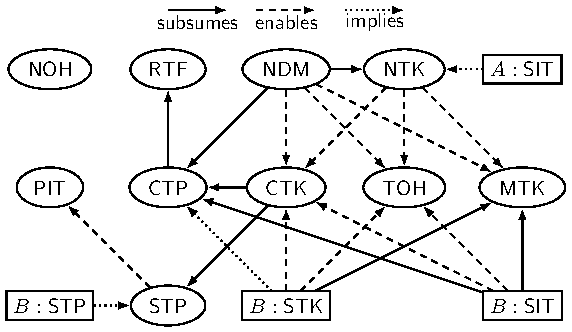
\includegraphics[scale = 0.7]{amass-dependency.pdf}
	\caption{Dependency graph for launch modes and intent flags in transitions $A \xrightarrow{\alpha(\phi)} B$. The launch modes %of $A$ and $B$ 
		(resp.\ the intent flags) are in boxes (resp. circles)}
		%in $\phi$
% \vspace{-6mm}	
	\label{fig-asm-depend}
\end{figure}


%%%%%%%%%%%%%%%%%%%%%%%%%%%%%%%%%%%%%%%%%%%%%%%
%%%%%%%%%%%%%%%%%%%%%%%%%%%%%%%%%%%%%%%%%%%%%%%
\hide{
\noindent\emph{\revision{understanding of the semantics}}

\revision{
For a given transition $A \xrightarrow{\startactivity(\phi)} B$.
Firstly, we consider two special cases, i.e., $\phi\models\tohflag$ and $\phi\models\mtkflag$, in these two cases, it need $\phi\models\ntkflag$.
\begin{itemize}
    \item If $\phi\models\tohflag$, it will clear up all the non-top tasks.
    \item If $\phi\models\mtkflag$, it will always launch a new task for $B$, except $\lmd(B) = \SIT/\STK$, since there is only one task with the real activity $B$ for the $\SIT$ or $\STK$ activity $B$.
\end{itemize}
Then we let $\phi\models\neg\tohflag\wedge\neg\mtkflag$, our semantics could be understood through the following mechanism:
\begin{enumerate}
    \item Determine which task will be associated with the caller activity $B$,
    \begin{itemize}
        \item If $\phi \models \ntkflag$ or if certain cases imply this, i.e., $\lmd(A) = \SIT$, $\lmd(B) = \SIT/\STK$, we need to specify a task that belongs to $B$ through the task allocation mechanism. If a task $S_i$ is found, then move the task $S_i$ to the top and proceed to step 2. Otherwise, launch a new task with $B$.
        \item Otherwise, proceed to step 2.
    \end{itemize}
    \item Determine how to place $B$ on top task, 
    \begin{itemize}
        \item If $\phi\models\neg\ctkflag\wedge\neg\ctpflag\wedge\neg\rtfflag$, then if the real activity of the top task or the top task is the main task, $B$ will be pushed into the top task.
        \item Otherwise $B$ is placed on the top task according to the dependencies between the launch mode of $B$ and the intent flags $\phi$. 
    \end{itemize}
\end{enumerate}
}
}
%%%%%%%%%%%%%%%%%%%%%%%%%%%%%%%%%%%%%%%%%%%%%%%
%%%%%%%%%%%%%%%%%%%%%%%%%%%%%%%%%%%%%%%%%%%%%%%


%Before describing the formal semantics, let us explain the intuition first.
%The system maintains fragment stack as well as transaction stack. 

%As mentioned in Section~\ref{sec:amm}, an activity %can be a plain activity meaning that it is unstructured and should be considered as atomic, or 
%contains sub-components 
%is structured and  in this paper we particularly focus on fragments. 
%Intuitively, %if 
%an activity contains a set of fragment containers each of which is associated with a \emph{fragment stack}, and features an \emph{transaction stack}. % to be used for defining the semantics of the action $\back$.)

%%%%%%%%%%%%%%%%%%%%%%%%%%%%%%%%%%%%%%%%%%%%%%%
%%%%%%%%%%%%%%%%%%%%%%%%%%%%%%%%%%%%%%%%%%%%%%%
\hide{
\subsection{Case $\tau = A \xrightarrow{\startactivity(\phi)} B$ and $\ell = 0$}
In this case, we distinguish two subcases, i.e., %Here we first assume that 
$\phi \models \neg \tohflag$ or $\phi \models \tohflag$. %We start with the first subcase. 

\subsection*{Case $\phi \models \neg \tohflag$}

%=================================================================================

\noindent {\fbox{$\lmd(B) = \singleinstance$}}
\begin{itemize}
	\item if $\getrealtsk(\rho, B) = S_i$ for some $i \in [n]$, 
        \begin{itemize}
            \item if $\phi\models\neg\ctkflag$, then $(\rho',\ell') = (\mvtsktop(\rho,i),0)$, $\jmath = (1,1)$ if $i = 1$, $\jmath = (2,1)$ otherwise,
            \item if $\phi\models\ctkflag$, then $(\rho',\ell') = (\clrtsk(\mvtsktop(\rho, i), B),\phi\models\nohflag)$, $\jmath = \bot$ if $i = 1$, $\jmath = (2,1)$ otherwise,
            % \item if $\phi\models\ctkflag\wedge\nohflag$, then $(\rho',\ell') = (\clrtsk(\mvtsktop(\rho, i), B),1)$, $\jmath = \bot$ if $i = 1$, $\jmath = (2,1)$ otherwise,
        \end{itemize}
	\item if $\getrealtsk(\rho, B) = *$, then $(\rho',\ell') = (\newtsk(\rho, B,\SIT),\phi\models\nohflag)$, $\jmath = (2,1)$.
	% \begin{itemize}
	% 	\item if $\phi\models\neg\nohflag$, then $(\rho',\ell') = (\newtsk(\rho, B),0)$,
	% 	\item if $\phi\models\nohflag$, then $(\rho',\ell') = (\newtsk(\rho, B),1)$.
	% \end{itemize}
\end{itemize}

\noindent {\fbox{$\lmd(B) = \singletask$}}
\begin{itemize}
	\item if $\getrealtsk(\rho, B) = S_i$ 
	or $ \getrealtsk(\rho, B) = * \wedge \gettsk(\rho, B) = S_i$, 
	\begin{itemize}
		\item if $\phi \models \neg \ctkflag $, 
		\begin{itemize}
			\item if $B \not \in S_i$, then $(\rho',\ell') = (\push(\mvtsktop(\rho,i),B),\phi\models\nohflag)$, $\jmath = (1,2)$ if $i = 1$, $\jmath = (2,1)$ otherwise,
			\item if $B \in S_i$, 	
			\begin{itemize}
				\item if $i = 1$ and $B = \topact(S_i)$, then $(\rho',\ell') = (\rho,0)$, $\jmath = (1,1)$,
				\item if $i = 1$ and $B \neq \topact(S_i)$, then $(\rho',\ell') = (\rho,0)$, $\jmath = \bot$,
				\item if $i \neq 1$, then $(\rho',\ell') = (\clrtop(\mvtsktop(\rho,i),B), 0)$, $\jmath = (2,1)$,
			\end{itemize}
		\end{itemize}
		\item if $\phi \models \ctkflag$, then $(\rho',\ell') = (\clrtsk(\mvtsktop(\rho, i), B),\phi\models\nohflag)$, $\jmath = \bot$ if $i = 1$, $\jmath = (2,1)$ otherwise,
	\end{itemize}
\item if $\gettsk(\rho, B) = *$, then $(\rho',\ell') = (\newtsk(\rho, B, \ntkflag),\phi\models\nohflag)$, $\jmath = (2,1)$.
\end{itemize}

\noindent {\fbox{$\lmd(B) = \standard$}}
\begin{itemize}
	\item if $\lmd(A) \neq \singleinstance$ and $\phi \models \neg \ntkflag$, 
	\begin{itemize}
        \item if $\phi\models\stpflag$ and $\topact(\rho) = B$, or $\phi\models\stpflag\wedge\pitflag$ and $\preact(\rho) = B$ , then $(\rho',\ell')=(\rho,0)$, $\jmath = (1,1)$,
        \item if $\phi\models\neg\stpflag\wedge\neg\rtfflag\wedge\neg\ctpflag$,
            or $\phi\models\stpflag\wedge\neg\rtfflag\wedge\neg\ctpflag$ and $B\neq\topact(\rho)$,
            or $\phi\models\stpflag\wedge\pitflag\wedge\neg\rtfflag\wedge\neg\ctpflag$ and $B\neq\preact(\rho)$,
            or $B\notin\toptsk(\rho)$,
                then $(\rho',\ell')=(\push(\rho, B),\phi\models\nohflag)$, $\jmath = (1,2)$,
        \item if $\phi \models \rtfflag \wedge \neg \ctpflag$ and $B \in \toptsk(\rho)$, then
         $(\rho',\ell')=(\mvacttop(\rho, B),0)$, $\jmath = (1,1)$ if $B = \topact(\rho)$, $\jmath = (1,2)$ otherwise,
        \item if $\phi \models\ctpflag\wedge\neg\stpflag$ and $B \in \toptsk(\rho)$, then
        $(\rho',\ell') =(\clrtop^*(\rho, B),\phi\models\nohflag)$, $\jmath = \bot$,
        \item if $\phi \models\ctpflag\wedge\stpflag$ and $B \in \toptsk(\rho)$, then
        $(\rho',\ell') =(\clrtop(\rho, B),0)$, $\jmath = (1,1)$ if $B = \topact(\rho)$, $\jmath = \bot$ otherwise,
	\end{itemize}
	\item if $\phi \models \ntkflag\wedge  \mtkflag\wedge\neg\ndmflag$, or $\lmd(A) = \singleinstance$ and $\phi \models \mtkflag\wedge\neg\ndmflag$,  then $(\rho',\ell') = (\newtsk(\rho, B, \ntkflag),\phi\models\nohflag)$, $\jmath = (2,1)$,
	\item if $\phi \models \ndmflag\wedge  \mtkflag$, then $(\rho',\ell') = (\newtsk(\rho, B, \ndmflag),\phi\models\nohflag)$, $\jmath = (2,1)$,
	\item if $\phi \models \ndmflag\wedge\neg\mtkflag$, 
    \begin{itemize}
        \item if $\getrealtsk(\rho,B) = S_i$, 
        \begin{itemize}
            \item if $\phi\models\neg\ctkflag$, then $(\rho',\ell')=(\clrtop(\mvtsktop(\rho,i), B),0)$, 
			\begin{itemize}
				\item if $i = 1$ and $B = \topact(\rho)$, then $\jmath = (1,1)$,
				\item if $i = 1$ and $B \neq \topact(\rho)$, then $\jmath = \bot$,
				\item if $i \neq 1$, then $\jmath = (2,1)$,
			\end{itemize}
            \item if $\phi\models\ctkflag$, then $(\rho',\ell') = (\clrtsk(\mvtsktop(\rho,i),B),\phi\models\nohflag)$, $\jmath = \bot$ if $i = 1$, $\jmath = (2,1)$ otherwise,
        \end{itemize}
        \item if $\getrealtsk(\rho,B) = *$, then $(\rho',\ell') = (\newtsk(\rho, B, \ndmflag),\phi\models\nohflag)$, $\jmath = (2,1)$,
    \end{itemize}
	%
	\item if $\phi \models \ntkflag\wedge \neg\ndmflag\wedge \neg \mtkflag$, or $\lmd(A) = \singleinstance$ and $\phi  \models \neg\ndmflag\wedge \neg \mtkflag$, then
	\begin{itemize}
        \item if $\getrealtsk(\rho, B) = S_i$ and $\zeta_i\neq\mainflag$,
            \begin{itemize}
            \item if $\phi\models\neg\ctkflag$ and $\topact(S_i) = B$, 
                or $\phi\models\neg\rtfflag\wedge\neg\ctpflag\wedge\neg\ctkflag$,
                then $(\rho',\ell')=(\mvtsktop(\rho, i), 0)$, $\jmath = (1,1)$ if $i = 1$, $\jmath = (2,1)$ otherwise,
            \item if $\phi\models(\rtfflag\vee\ctpflag)\wedge\neg\ctkflag$ and $B\notin S_i$,
				then $(\rho',\ell')=(\push(\mvtsktop(\rho, i), B),\phi\models\nohflag)$, $\jmath = (1,2)$ if $i = 1$, $\jmath = (2,1)$ otherwise,
            \item if $\phi \models \rtfflag \wedge \neg \ctpflag\wedge\neg\ctkflag$ and $B \in S_i$,
			then $(\rho',\ell')=(\mvacttop(\mvtsktop(\rho, i), B),0)$,
			\begin{itemize}
				\item if $i = 1$ and $B = \topact(\rho)$, then $\jmath = (1,1)$,
				\item if $i = 1$ and $B \neq \topact(\rho)$, then $\jmath = (1,2)$,
				\item if $i \neq 1$, then $\jmath = (2,1)$,
			\end{itemize}
            \item if $\phi \models\ctpflag\wedge\neg\stpflag\wedge\neg\ctkflag$ and $B \in S_i$, then $(\rho',\ell') =(\clrtop^*(\mvtsktop(\rho, i), B), \phi\models\nohflag)$, $\jmath = \bot$ if $i = 1$, $\jmath = (2,1)$ otherwise,
            \item if $\phi \models\ctpflag\wedge\stpflag\wedge\neg\ctkflag$ and $B \in S_i$, 
			then $(\rho',\ell') =(\clrtop(\mvtsktop(\rho, i), B), 0)$, 
			\begin{itemize}
				\item if $i = 1$ and $B = \topact(\rho)$, then $\jmath = (1,1)$,
				\item if $i = 1$ and $B \neq \topact(\rho)$, then $\jmath = \bot$,
				\item if $i \neq 1$, then $\jmath = (2,1)$,
			\end{itemize}
            \item if $\phi \models\ctkflag$, then
            $(\rho',\ell') = (\clrtsk(\mvtsktop(\rho, i), B),\phi\models\nohflag)$, $\jmath = \bot$ if $i = 1$, $\jmath = (2,1)$ otherwise,
            \end{itemize}
            \item if $\getrealtsk(\rho, B) = S_i$ and $\zeta_i=\mainflag$,
        or $ \getrealtsk(\rho, B) = * \wedge \gettsk(\rho, B) = S_i$, 
		\begin{itemize}
            \item if $\phi \models (\stpflag\vee\rtfflag\vee\ctpflag)\wedge\neg\ctkflag$ and $\topact(S_i) = B$,
            or $\phi \models \rtnflag \wedge\neg\rtfflag\wedge\neg\ctpflag\wedge\neg\ctkflag$,
			then $(\rho',\ell')=(\mvtsktop(\rho, i), 0)$, $\jmath = (1,1)$ if $i = 1$, $\jmath = (2,1)$ otherwise,
            \item if $\phi\models\neg\stpflag\wedge\neg\rtnflag\wedge\neg\rtfflag\wedge\neg\ctpflag\wedge\neg\ctkflag$,
                or $\phi\models\stpflag\wedge\neg\rtnflag\wedge\neg\rtfflag\wedge\neg\ctpflag\wedge\neg\ctkflag$ and $B\neq\topact(S_i)$,
                or $\phi\models\neg\rtnflag\wedge\neg\ctkflag$ and $B\notin S_i$,
				then $(\rho',\ell')=(\push(\mvtsktop(\rho, i), B),\phi\models\nohflag)$, $\jmath = (1,2)$ if $i = 1$, $\jmath = (2,1)$ otherwise,
            \item if $\phi \models \rtfflag \wedge \neg \ctpflag\wedge\neg\ctkflag$ and $B \in S_i$, 
			then $(\rho',\ell')=(\mvacttop(\mvtsktop(\rho, i), B),0)$,
			\begin{itemize}
				\item if $i = 1$ and $B = \topact(\rho)$, then $\jmath = (1,1)$,
				\item if $i = 1$ and $B \neq \topact(\rho)$, then $\jmath = (1,2)$,
				\item if $i \neq 1$, then $\jmath = (2,1)$,
			\end{itemize}
            \item if $\phi \models\ctpflag\wedge\neg\stpflag\wedge\neg\ctkflag$ and $B \in S_i$, then $(\rho',\ell') =(\clrtop^*(\mvtsktop(\rho, i), B), \phi\models\nohflag)$, $\jmath = \bot$ if $i = 1$, $\jmath = (2,1)$ otherwise,
            \item if $\phi \models\ctpflag\wedge\stpflag\wedge\neg\ctkflag$ and $B \in S_i$, then $(\rho',\ell') =(\clrtop(\mvtsktop(\rho, i), B), 0)$, 
			\begin{itemize}
				\item if $i = 1$ and $B = \topact(\rho)$, then $\jmath = (1,1)$,
				\item if $i = 1$ and $B \neq \topact(\rho)$, then $\jmath = \bot$,
				\item if $i \neq 1$, then $\jmath = (2,1)$,
			\end{itemize}
            \item if $\phi \models\ctkflag$, then
            $(\rho',\ell') = (\clrtsk(\mvtsktop(\rho, i), B),\phi\models\nohflag)$, $\jmath = \bot$ if $i = 1$, $\jmath = (2,1)$ otherwise,
		\end{itemize}
		\item if $\gettsk(\rho, B) = *$, then $(\rho',\ell') = (\newtsk(\rho, B, \ntkflag), \phi\models\nohflag)$, $\jmath = (2,1)$.
	\end{itemize}
\end{itemize}

\noindent  {\fbox{$\lmd(B) = \singletop$}}
\begin{itemize}
	\item if $\lmd(A) \neq \singleinstance$ and $\phi \models \neg \ntkflag\wedge\neg\ndmflag$, 
	\begin{itemize}
		\item if $\topact(\rho) = B$, or $\phi\models\pitflag$ and $\preact(\rho) = B$, then $(\rho',\ell')= (\rho,0)$, $\jmath = (1,1)$,
        \item if $\phi \models  \neg \rtfflag\wedge \neg \ctpflag$, and $B\neq\topact(\rho)$,
        or $\phi \models \pitflag\wedge\neg \rtfflag\wedge \neg \ctpflag$, and $B\neq\preact(\rho)$,
        or $B\notin \toptsk(\rho)$, then $(\rho',\ell')=(\push(\rho, B),\phi\models\nohflag)$, $\jmath = (1,2)$,
        %
        \item if $\phi \models \rtfflag \wedge \neg \ctpflag$ and $B \in \toptsk(\rho)$, then
         $(\rho',\ell')=(\mvacttop(\rho, B),0)$, $\jmath = (1,1)$ if $B = \topact(\rho)$, $\jmath = (1,2)$ otherwise,
        \item if $\phi \models\ctpflag$ and $B \in \toptsk(\rho)$, then
        $(\rho',\ell') =(\clrtop(\rho, B),0)$, $\jmath = (1,1)$ if $B = \topact(\rho)$, $\jmath = \bot$ otherwise,
	\end{itemize}
	\item if $\phi \models \ntkflag\wedge  \mtkflag\wedge\neg\ndmflag$, or $\lmd(A) = \singleinstance$ and $\phi \models \mtkflag\wedge\neg\ndmflag$,  then $(\rho',\ell') = (\newtsk(\rho, B, \ntkflag),\phi\models\nohflag)$, $\jmath = (2,1)$,
	\item if $\phi \models \ndmflag\wedge  \mtkflag$, then $(\rho',\ell') = (\newtsk(\rho, B, \ndmflag),\phi\models\nohflag)$, $\jmath = (2,1)$,
	\item if $\phi \models \ndmflag\wedge\neg\mtkflag$, 
    \begin{itemize}
        \item if $\getrealtsk(\rho,B) = S_i$, 
        \begin{itemize}
            \item if $\phi\models\neg\ctkflag$, then $(\rho',\ell')=(\clrtop(\mvtsktop(\rho,i), B),0)$, 
			\begin{itemize}
				\item if $i = 1$ and $B = \topact(\rho)$, then $\jmath = (1,1)$,
				\item if $i = 1$ and $B \neq \topact(\rho)$, then $\jmath = \bot$,
				\item if $i \neq 1$, then $\jmath = (2,1)$,
			\end{itemize}
            \item if $\phi\models\ctkflag$, then $(\rho',\ell') = (\clrtsk(\mvtsktop(\rho,i),B),\nohflag)$, $\jmath = \bot$ if $i = 1$, $\jmath = (2,1)$ otherwise,
        \end{itemize}
        \item if $\getrealtsk(\rho,B) = *$, then $(\rho',\ell') = (\newtsk(\rho, B, \ndmflag),\phi\models\nohflag)$, $\jmath = (2,1)$,
    \end{itemize}
	%
	\item if $\phi \models \ntkflag\wedge\neg\ndmflag\wedge \neg \mtkflag$, or $\lmd(A) = \singleinstance$ and $\phi  \models\neg\ndmflag\wedge \neg \mtkflag$, then
	\begin{itemize}
        \item if $\getrealtsk(\rho, B) = S_i$ and $\zeta_i\neq\mainflag$,
            \begin{itemize}
            \item if $\phi\models\neg\ctkflag$ and $\topact(S_i) = B$, 
                or $\phi\models\neg\rtfflag\wedge\neg\ctpflag\wedge\neg\ctkflag$,
                then $(\rho',\ell')=(\mvtsktop(\rho, i), 0)$, $\jmath = (1,1)$ if $i = 1$, $\jmath = (2,1)$ otherwise,
            \item if $\phi\models(\rtfflag\vee\ctpflag)\wedge\neg\ctkflag$ and $B\notin S_i$, 
				then $(\rho',\ell')=(\push(\mvtsktop(\rho, i), B),\phi\models\nohflag)$, $\jmath = (1,2)$ if $i = 1$, $\jmath = (2,1)$ otherwise,
            \item if $\phi \models \rtfflag \wedge \neg \ctpflag\wedge\neg\ctkflag$ and $B \in S_i$,
			then $(\rho',\ell')=(\mvacttop(\mvtsktop(\rho, i), B),0)$,
			\begin{itemize}
				\item if $i = 1$ and $B = \topact(\rho)$, then $\jmath = (1,1)$,
				\item if $i = 1$ and $B \neq \topact(\rho)$, then $\jmath = (1,2)$,
				\item if $i \neq 1$, then $\jmath = (2,1)$,
			\end{itemize}
            \item if $\phi \models\ctpflag\wedge\neg\ctkflag$ and $B \in S_i$, 
			then $(\rho',\ell') =(\clrtop(\mvtsktop(\rho, i), B), 0)$, 
			\begin{itemize}
				\item if $i = 1$ and $B = \topact(\rho)$, then $\jmath = (1,1)$,
				\item if $i = 1$ and $B \neq \topact(\rho)$, then $\jmath = \bot$,
				\item if $i \neq 1$, then $\jmath = (2,1)$,
			\end{itemize}
            \item if $\phi \models\ctkflag$, 
			then $(\rho',\ell') = (\clrtsk(\mvtsktop(\rho, i), B),\phi\models\nohflag)$, $\jmath = \bot$ if $i = 1$, $\jmath = (2,1)$ otherwise,
            \end{itemize}
            \item if $\getrealtsk(\rho, B) = S_i$ and $\zeta_i=\mainflag$,
        or $ \getrealtsk(\rho, B) = * \wedge \gettsk(\rho, B) = S_i$, 
		\begin{itemize}
            \item if $\phi \models \neg\ctkflag$ and $\topact(S_i) = B$, 
            or $\phi\models\rtnflag\wedge\neg\rtfflag\wedge\neg\ctpflag\wedge\neg\ctkflag$,
			then $(\rho',\ell')=(\mvtsktop(\rho, i), 0)$, $\jmath = (1,1)$ if $i = 1$, $\jmath = (2,1)$ otherwise,
            \item if $\phi\models\neg\rtnflag\wedge\neg\rtfflag\wedge\neg\ctpflag\wedge\neg\ctkflag$ and $B\neq\topact(S_i)$,
			or $\phi\models\neg\rtnflag\wedge\neg\ctkflag$ and $B\notin S_i$,
			then $(\rho',\ell')=(\push(\mvtsktop(\rho, i), B),\phi\models\nohflag)$, $\jmath = (1,2)$ if $i = 1$, $\jmath = (2,1)$ otherwise,
            \item if $\phi \models \rtfflag \wedge \neg \ctpflag\wedge\neg\ctkflag$ and $B \in S_i$, then 
			then $(\rho',\ell')=(\mvacttop(\mvtsktop(\rho, i), B),0)$,
			\begin{itemize}
				\item if $i = 1$ and $B = \topact(\rho)$, then $\jmath = (1,1)$,
				\item if $i = 1$ and $B \neq \topact(\rho)$, then $\jmath = (1,2)$,
				\item if $i \neq 1$, then $\jmath = (2,1)$,
			\end{itemize}
            \item if $\phi \models\ctpflag\wedge\neg\ctkflag$ and $B \in S_i$, 
			then $(\rho',\ell') =(\clrtop(\mvtsktop(\rho, i), B), 0)$, 
			\begin{itemize}
				\item if $i = 1$ and $B = \topact(\rho)$, then $\jmath = (1,1)$,
				\item if $i = 1$ and $B \neq \topact(\rho)$, then $\jmath = \bot$,
				\item if $i \neq 1$, then $\jmath = (2,1)$,
			\end{itemize}
            \item if $\phi \models\ctkflag$,
			then $(\rho',\ell') = (\clrtsk(\mvtsktop(\rho, i), B),\phi\models\nohflag)$, $\jmath = \bot$ if $i = 1$, $\jmath = (2,1)$ otherwise,
		\end{itemize}
		\item if $\gettsk(\rho, B) = *$, then $(\rho',\ell') = (\newtsk(\rho, B, \ntkflag), \phi\models\nohflag)$, $\jmath = (2,1)$.
	\end{itemize}
	
\end{itemize}


%%%%%%%%%%%%%%%%%%%%%%%%%%%%%%%%%%%%%%%%%%%%%%%%%%%%%%%%%%%%%%%%%%%%%%%%%%%%%%%%%%%%%%%%%%%%%%%%%%%
\subsection*{Case $\phi \models \tohflag$}
%
We then consider the transition rules $\tau =A \xrightarrow{\startactivity(\phi)} B$ with $\phi \models \tohflag\wedge(\ntkflag\vee\ndmflag)$, 
or $\lmd(A) = \singleinstance$ and $\phi\models\tohflag$,
or $\lmd(B) = \singleinstance/\singletask$ and $\phi\models\tohflag$. It turns out that we can largely reuse the semantic definitions of the case that $\phi \models \neg \tohflag$. Namely, 
let $\tau' = A \xrightarrow{\startactivity(\phi')} B$ where $\phi'$ is obtained from $\phi$ by replacing $\tohflag$ with $\neg \tohflag$. (The behavior of $\tau'$ is fully prescribed before, viz, $(\rho,\ell) \xrightarrow[\tau',\jmath']{\Mm} (\rho',\ell')$ where $\rho' = ((S'_1, A'_1,\zeta'_1), \cdots, (S'_{n'}, A'_{n'},\zeta'_{n'}))$. Then we have that $(\rho,\ell) \xrightarrow[\tau,\jmath]{\Mm} ((S'_1, A'_1,\zeta'_1))$ and $\jmath = \bot$ if $\jmath' = (2,1)$, $\jmath = \jmath'$ otherwise.

%\smallskip
%\noindent \fbox{Case $\tau = A \xrightarrow{\finishstart(\phi)} B$}
%\smallskip
\subsection{Case $\tau = A \xrightarrow{\finishstart(\phi)} B$}

In this case, $A\xrightarrow {\finishstart(\phi)}B$ specifies that $B$ is started with the intent flags $\phi$ followed by the termination of $A$, popped from the task stack. Let
%Suppose that $\rho$ is the current configuration with 
%$\rho=((S_1,A_1,b_1), \cdots, (S_n, A_n, b_n))$, let $S_1=[A]\cdot S_1'$, where $S_1'\in\act^*$.
$\tau' = A \xrightarrow {\startactivity(\phi)}B$ and $(\rho,0) \xrightarrow[\tau',\jmath]{\Mm} (\rho'',\ell'')$, then we have $(\rho,\ell) \xrightarrow[\tau,\jmath]{\Mm} (\rho',\ell'')$, where $\rho = \rmact(\rho'', x, y)$ if $\jmath = (x, y)$, $\rho' = \rho''$ otherwise.

\subsection{Case $\tau = A \xrightarrow{\alpha(\phi)} B$ and $\ell = 1$}

Similarly, it specifies that $B$ is started with the intent flags $\phi$ followed by the termination of $A$, popped from the task stack. Let
$(\rho,0) \xrightarrow[\tau,\jmath]{\Mm} (\rho'',\ell'')$, then we have $(\rho,1) \xrightarrow[\tau,\jmath]{\Mm} (\rho',\ell'')$, where $\rho = \rmact(\rho'', x, y)$ if $\jmath = (x, y)$, $\rho' = \rho''$ otherwise.

%then $\rho \xrightarrow[\tau]{\Mm} \rho'$, where $\rho''\xrightarrow[\tau']{\Mm}\rho'$ and $\rho''$ is defined as follows:
%\begin{itemize}
%    \item if $|S_1'|>0$, then $\rho''=( (S_1',A_1,b_1)\cdots,(S_n,A_n,b_n) )$,
%    \item otherwise, $\rho''=( (S_2,A_2,b_2)\cdots,(S_n,A_n,b_n) )$.
%\end{itemize}
%Then we have $\rho \xrightarrow[\tau]{\Mm} \rho'$.

%Proposition~\ref{prop:sem} reassures that $\xrightarrow{\Aa}$ is indeed a relation on $\conf_\Aa$ as per Definition~\ref{def-ass-conf}.
%
%\begin{proposition} \label{prop:sem}
%	Let $\Aa$ be an ASM. For each $(q, \rho) \in \conf_\Aa$ and  $(q, \rho) \xrightarrow{\Aa} (q', \rho')$,
%	$(q', \rho') \in \conf_\Aa$, namely, $(q', \rho')$  satisfies the five constraints in Definition~\ref{def-ass-conf}.
%\end{proposition}


%\noindent\hlfancyfancy{$\mathcolorbox{highlightcolor}{\mbox{Case }\tau = A \xrightarrow{\opstack} (\beta_1(F_1, i_1), \cdots, \beta_k(F_k, i_k))}$}
%\noindent\fbox{Case $\tau = A \xrightarrow{\opstack} (\beta_1(F_1, i_1), \cdots, \beta_k(F_k, i_k))$}
%\smallskip


\subsection{Case $\tau = A \xrightarrow{\opstack} (\beta_1(F_1, i_1, x_1), \cdots, \beta_k(F_k, i_k, x_k))$}\ 

%Suppose $S_1 = [(B_1, \Theta_1), \cdots, (B_r, \Theta_r)]$ (where $B_1 = A$ and $\Theta_1 = \Theta$). 
In this case, 
let $T = (\beta_1(F_1, i_1, x_1), \cdots, \beta_k(F_k, i_k, x_k))$. 
Then we have $(\rho,\ell) \xrightarrow[\tau,(1,1)]{\Mm} (\rho',\ell)$, where
%$i=1$, $\ell' = \ell$, and 
$$\rho' = ((S'_1, A_1,\zeta_1), (S_2, A_2,\zeta_2), \cdots, (S_n, A_n,\zeta_n))$$ is obtained from $\rho$ by applying all the actions in $T$ to the containers and assignment function in $\Theta=\Theta_1$ (recall that $\tact(S_1) = (A, \Theta)$), specifically,  
$S'_1 =[(B_1, \Theta'_1), (B_2, \Theta_2), \cdots, (B_r, \Theta_r)],$ 
where $\Theta'_1 = (\upsilon', \eta', \iota')$ such that $(\upsilon', \iota') = \updateviews_{T}(\upsilon, \iota)$ and $\eta' = \concaction_{\upsilon, \iota}(T) \cdot \eta$.

%\smallskip 
%\noindent\fbox{Case $\tau = A \xrightarrow{\nopstack} (\beta_1(F_1, i_1), \cdots, \beta_k(F_k, i_k))$}
%\smallskip
 
%Suppose $S_1 = [(B_1, \Theta_1), \cdots, (B_r, \Theta_r)]$ (where $B_1 = A$ and $\Theta_1 = \Theta$). 

\subsection{Case $\tau = A \xrightarrow{\nopstack} (\beta_1(F_1, i_1, x_1), \cdots, \beta_k(F_k, i_k, x_k))$}\ 

In this case, let $T = (\beta_1(F_1, i_1, x_1), \cdots, \beta_k(F_k, i_k, x_k))$,
Then we have $(\rho,\ell) \xrightarrow[\tau,(1,1)]{\Mm} (\rho',\ell)$, where
$$\rho' = ((S'_1, A_1,\zeta_1), (S_2, A_2,\zeta_2), \cdots, (S_n, A_n,\zeta_n))$$ such that 
$$S'_1 =[(B_1, \Theta'_1), (B_2, \Theta_2), \cdots, (B_r, \Theta_r)],$$ 
where $\Theta'_1 = (\upsilon', \eta, \iota')$, and $(\upsilon', \iota') = \updateviews_{T}(\upsilon, \iota)$. Note that in this case, the concretization of $T$ is not stored into the transaction stack. 

%\smallskip
%\noindent \fbox{Case $\tau = \back$}
%\smallskip

\subsection{Case $\tau = \back$}
In this case, we distinguish two subcases, i.e., $\eta=\epsilon$ or $\eta\neq\epsilon$.
\subsection*{Case $\eta=\epsilon$}
In this case, if $S_1$ contains exactly one activity (i.e. $A$), then $S_1$ disappears after the $\back$ action, that is, $(\rho,\ell) \xrightarrow[\tau,\bot]{\Mm} (\rho',0)$, where $\rho' = ((S_2, A_2,\zeta_2), \cdots, (S_n, A_n,\zeta_n))$.
On the other hand, if $S_1$ contains at least two activities, then $(\rho,\ell) \xrightarrow[\tau,\bot]{\Mm} (\rho',0)$, where $\rho' = ((S'_1,A_1,\zeta_1), (S_2, A_2,\zeta_2), \cdots, (S_n, A_n,\zeta_n))$ and $S'_1$ is obtained from $S_1$ by removing the top activity $A$ from $S_1$.
\subsection*{Case $\eta\neq\epsilon$}
In this case, 
$(\rho,\ell) \xrightarrow[\tau,(1,1)]{\Mm} (\rho',\ell)$, where %$i = 1$, $\ell' = \ell$, and 
$$\rho' = ((S'_1, A_1,\zeta_1), (S_2, A_2,\zeta_2), \cdots, (S_n, A_n,\zeta_n))$$
such that 
$$S'_1 =[(B_1, \Theta'_1), (B_2, \Theta_2), \cdots, (B_r, \Theta_r)],$$ 
where 
$\Theta'_1 = (\upsilon', \eta', \iota')$, $(\upsilon', \iota') = \updateviews_{T_1^{-1}}(\upsilon, \iota),$ and $\eta' = (T_2, \cdots, T_l)$.
Note that $T_1$ is popped off the transaction stack and the actions of $T_1$ are revoked on $(\upsilon, \iota)$.
 

%%%%%%%%%%%%%%%%%%%%%%%%%%%%%%%%%%%%%%%%%%
\subsection{Other cases}
When $\upsilon \neq (\epsilon, \cdots, \epsilon)$, the fragment stacks of $A$ contains at least one fragment and the transition rules of the following form are applicable, namely,  $F \xrightarrow{\startactivity(\phi)} B$, $ F \xrightarrow{\finishstart(\phi)} B$,  $F \xrightarrow{\opstack} (\beta_1(F_1, i_1, x_1), \cdots, \beta_k(F_k, i_k, x_k))$, and $F \xrightarrow{\nopstack} (\beta_1(F_1, i_1, x_1), \cdots, \beta_k(F_k, i_k, x_k))$  with $F \in \tfrag(\upsilon)$. 
The semantics of these rules are similar to those of the case of the source is activity.
}
%We will focus on the transition rules $\tau = F \xrightarrow{\mu} (\beta_1(F_1, i_1), \cdots, \beta_k(F_k, i_k))$ (where $\mu \in \{\opstack, \nopstack\}$) 
%$F \xrightarrow{\nopstack} (\beta_1(F_1, i_1), \cdots, \beta_k(F_k, i_k))$, 
%The semantics of the other rules are similar to those of the case $v=(\epsilon,\cdots,\epsilon)$ above.
%$A \xrightarrow{\mu} (\beta_1(F_1, i_1), \cdots, \beta_k(F_k, i_k))$ above.
\hide{
Suppose $S_1 = [(B_1, \Theta_1), \cdots, (B_r, \Theta_r)]$ (where $B_1 = A$ and $\Theta_1 = \Theta$). 
\smallskip
\noindent\fbox{Case $\tau = F \xrightarrow{\opstack} (\beta_1(F_1, i_1), \cdots, \beta_k(F_k, i_k))$}
 

%Suppose $S_1 = [(B_1, \Theta_1), \cdots, (B_r, \Theta_r)]$ (where $B_1 = A$ and $\Theta_1 = \Theta$). 

Let $T = (\beta_1(F_1, i_1), \cdots, \beta_k(F_k, i_k))$. 
In this case, $\rho \xrightarrow[\tau]{\Mm} \rho'$, where 
$$\rho' = ((S'_1, A_1,b_1), (S_2, A_2,b_2), \cdots, (S_n, A_n,b_n))$$
such that $S'_1 =[(B_1, \Theta'_1), (B_2, \Theta_2), \cdots, (B_r, \Theta_r)]$, $\Theta'_1 = (\upsilon', \eta')$, $\upsilon' = \updateviews^\sharp_{T}(\upsilon)$, and $\eta' = \concaction^\sharp_\upsilon(T) \cdot \eta$.

  \smallskip
\noindent\fbox{Case $\tau = F \xrightarrow{\nopstack} (\beta_1(F_1, i_1), \cdots, \beta_k(F_k, i_k))$}
 


%Suppose $S_1 = [(B_1, \Theta_1), \cdots, (B_r, \Theta_r)]$ (where $B_1 = A$ and $\Theta_1 = \Theta$). 

Let $T = (\beta_1(F_1, i_1), \cdots, \beta_k(F_k, i_k))$. 
In this case, $\rho \xrightarrow[\tau]{\Mm} \rho'$, where 
$$\rho' = ((S'_1, A_1,b_1), (S_2, A_2,b_2), \cdots, (S_n, A_n,b_n))$$
such that $S'_1 =[(B_1, \Theta'_1), (B_2, \Theta_2), \cdots, (B_r, \Theta_r)]$, $\Theta'_1 = (\upsilon', \eta)$, and $\upsilon' = \updateviews_{T}(\upsilon)$.
}
%%%%%%%%%%%%%%%%%%%%%%%%%%%%%%%%%%%%%%%%%%%%%%%
%%%%%%%%%%%%%%%%%%%%%%%%%%%%%%%%%%%%%%%%%%%%%%%


\section{Semantics of {\AMASS} models for the other versions of Android}
%
We state the differences of the semantics of {$\AMASS$} models in details. To avoid tediousness, let us focus on the situation $\phi \models \neg \tohflag$. The differences for the situation $\phi \models \tohflag$ are similar. 

\subsection{Android 11.0 and 12.0.}
The semantics of {\AMASS} for Android 11.0 and 12.0 are the same as Android 13.0. 

\subsection{Android 10.0, 9.0, and 8.0.}
The semantics for these three versions are the same and differ from that for Android 13.0 in the following sense: $\rtfflag$ is ignored when used together with $\ntkflag$ or $\lmd(A) = \SIT$. 
That is, for Android 10.0, 9.0, and 8.0, the semantics of $\AMASS$ for the case $\lmd(B) = \STD$ and $\phi \models \ntkflag \wedge \neg \ndmflag\wedge \neg \mtkflag$, or $\lmd(A) = \SIT$ and $\phi \models \neg\ndmflag\wedge\neg\mtkflag$, is adapted from Android 13.0 as follows.

%When $\phi \models \ntkflag \wedge \neg\ndmflag\wedge\neg \mtkflag$, $\rtfflag$ is ignored. 
%
\begin{itemize}
    \item if $\getrealtsk(\rho, B) = S_i$ or $\getrealtsk(\rho,B) = * \wedge\gettsk(\rho,B) = S_i$, then
    \begin{itemize}
    \item if $i \neq 1$, then 
        \begin{itemize}
            \item if $\phi \models \ctkflag$, then $\cdots$ 
            \item if $\phi \models \neg \ctkflag$, then $\cdots$
                \begin{itemize}
                    \item if $\phi \models\ctpflag$ and $B \in S_i$, then $\cdots$
                    \item if $\phi \models\ctpflag$ and $B \notin S_i$, then $\cdots$
                    \item if $\phi \models\neg\ctpflag$, then
                    \begin{itemize}
							\item if $\getrealtsk(\rho,B) = S_i$ and $\zeta_i \neq \mainflag$, then $b' = \neg \nohflag$, moreover,
							\begin{itemize}
								\item if $b = \neg \nohflag$ and $\alpha = \startactivity$, then $\rho'=\mvtsktop(\rho, i)$,
								\item otherwise, $\rho' = \rmact(\mvtsktop(\rho, i), 2, 1)$, 
							\end{itemize}
							\item otherwise ($\getrealtsk(\rho,B) = S_i$ and $\zeta_i = \mainflag$ or $\getrealtsk(\rho,B) = * \wedge\gettsk(\rho,B) = S_i$), 
							\begin{itemize}
								\item if $\phi\models\stpflag$ and $\topact(S_i) = B$, then $b' = \neg \nohflag$, moreover,
								\begin{itemize}
									\item if $b = \neg \nohflag$ and $\alpha = \startactivity$, then $\rho'=\mvtsktop(\rho, i)$,
									\item otherwise, $\rho' = \rmact(\mvtsktop(\rho, i), 2, 1)$, 
								\end{itemize}
								\item otherwise, $b' = \nohflag$ iff $\phi \models \nohflag$, moreover, 
								\begin{itemize}
									\item if $b = \neg \nohflag$ and $\alpha = \startactivity$, then $\rho'=\push(\mvtsktop(\rho, i), B)$,
									\item otherwise, $\rho' = \rmact(\push(\mvtsktop(\rho, i), B), 2, 1)$, 
								\end{itemize}
							\end{itemize}
                    \end{itemize}
                \end{itemize}
        \end{itemize}
    \item otherwise ($i  = 1$),  
    \begin{itemize}
        \item if $\phi \models \ctkflag$, then $\cdots$, 
        \item if $\phi \models \neg \ctkflag$, then 
        \begin{itemize}
            \item if $\phi \models \ctpflag$ and $B \in S_1$, then $\cdots$
%				\begin{itemize}
%					\item if $\phi\models \neg \stpflag$, then $b' = \nohflag$ iff $\phi \models \nohflag$, 
%					\item otherwise, $b' = \neg \nohflag$,
%				\end{itemize}
            \item if $\phi \models \ctpflag$ and $B\notin S_1$, then $\cdots$
            \item if $\phi \models \neg \ctpflag$, then
            \begin{itemize}
				\item if $\getrealtsk(\rho,B) = S_1$ and $\zeta_1 \neq \mainflag$, 
				\begin{itemize}
					\item if $\alpha = \startactivity$, then $\rho' = \rho$ and $b' = b$,
					\item if $\alpha = \finishstart$, then $\rho' = \rmact(\rho, 1, 1)$ and $b' = \neg\nohflag$,
				\end{itemize}
			\item otherwise ($\getrealtsk(\rho,B) = S_1$ and $\zeta_i = \mainflag$ or $\getrealtsk(\rho,B) = * \wedge\gettsk(\rho,B) = S_1$), 
			\begin{itemize}
				\item if $\phi\models\stpflag$ and $A = B$, or $\phi \models\stpflag\wedge\pitflag$ and $\preact(\rho) = B$, 
				\begin{itemize}
					\item if $\alpha = \startactivity$, then $\rho' = \rho$ and $b' = b$,
					\item if $\alpha = \finishstart$, then $\rho' = \rmact(\rho, 1, 1)$ and $b' = \neg\nohflag$,
				\end{itemize}
				\item otherwise, $b' = \nohflag$ iff $\phi \models \nohflag$, moreover, 
				\begin{itemize}
					\item if $b = \neg \nohflag$ and $\alpha = \startactivity$, then $\rho'=\push(\rho, B)$,
					\item otherwise, $\rho' = \rmact(\push(\rho, B), 1, 2)$, 
				\end{itemize}
			\end{itemize}
            \end{itemize}
        \end{itemize}
    \end{itemize}
\end{itemize}
\item if $\gettsk(\rho, B) = *$, then $\cdots$. 
\end{itemize}
Similarly the semantics of $\AMASS$ for the case $\lmd(B) = \STP$ and $\phi \models \ntkflag \wedge \neg \ndmflag\wedge \neg \mtkflag$ or $\lmd(A) = \SIT$ and $\phi \models \neg\ndmflag\wedge\neg\mtkflag$ is adapted from Android 13.0 as follows.

\begin{itemize}
    \item if $\getrealtsk(\rho, B) = S_i$ or $\getrealtsk(\rho,B) = * \wedge\gettsk(\rho,B) = S_i$, then
    \begin{itemize}
    \item if $i \neq 1$, then 
        \begin{itemize}
            \item if $\phi \models \ctkflag$, then $\cdots$ 
            \item if $\phi \models \neg \ctkflag$, then $\cdots$
                \begin{itemize}
                    \item if $\phi \models\ctpflag$ and $B \in S_i$, then $\cdots$
                    \item if $\phi \models\ctpflag$ and $B \notin S_i$, then $\cdots$
                    \item if $\phi \models\neg\ctpflag$, then
                    \begin{itemize}
							\item if $\getrealtsk(\rho,B) = S_i$ and $\zeta_i \neq \mainflag$, then $b' = \neg \nohflag$, moreover,
							\begin{itemize}
								\item if $b = \neg \nohflag$ and $\alpha = \startactivity$, then $\rho'=\mvtsktop(\rho, i)$,
								\item otherwise, $\rho' = \rmact(\mvtsktop(\rho, i), 2, 1)$, 
							\end{itemize}
							\item otherwise ($\getrealtsk(\rho,B) = S_i$ and $\zeta_i = \mainflag$ or $\getrealtsk(\rho,B) = * \wedge\gettsk(\rho,B) = S_i$), 
							\begin{itemize}
								\item if $\topact(S_i) = B$, then $b' = \neg \nohflag$, moreover,
								\begin{itemize}
									\item if $b = \neg \nohflag$ and $\alpha = \startactivity$, then $\rho'=\mvtsktop(\rho, i)$,
									\item otherwise, $\rho' = \rmact(\mvtsktop(\rho, i), 2, 1)$, 
								\end{itemize}
								\item otherwise, $b' = \nohflag$ iff $\phi \models \nohflag$, moreover, 
								\begin{itemize}
									\item if $b = \neg \nohflag$ and $\alpha = \startactivity$, then $\rho'=\push(\mvtsktop(\rho, i), B)$,
									\item otherwise, $\rho' = \rmact(\push(\mvtsktop(\rho, i), B), 2, 1)$, 
								\end{itemize}
							\end{itemize}
                    \end{itemize}
                \end{itemize}
        \end{itemize}
    \item otherwise ($i  = 1$),  
    \begin{itemize}
        \item if $\phi \models \ctkflag$, then $\cdots$, 
        \item if $\phi \models \neg \ctkflag$, then 
        \begin{itemize}
            \item if $\phi \models \ctpflag$ and $B \in S_1$, then $\cdots$
%				\begin{itemize}
%					\item if $\phi\models \neg \stpflag$, then $b' = \nohflag$ iff $\phi \models \nohflag$, 
%					\item otherwise, $b' = \neg \nohflag$,
%				\end{itemize}
            \item if $\phi \models \ctpflag$ and $B\notin S_1$, then $\cdots$
            \item if $\phi \models \neg \ctpflag$, then
            \begin{itemize}
				\item if $\getrealtsk(\rho,B) = S_1$ and $\zeta_1 \neq \mainflag$, 
				\begin{itemize}
					\item if $\alpha = \startactivity$, then $\rho' = \rho$ and $b' = b$,
					\item if $\alpha = \finishstart$, then $\rho' = \rmact(\rho, 1, 1)$ and $b' = \neg\nohflag$,
				\end{itemize}
			\item otherwise ($\getrealtsk(\rho,B) = S_1$ and $\zeta_i = \mainflag$ or $\getrealtsk(\rho,B) = * \wedge\gettsk(\rho,B) = S_1$), 
			\begin{itemize}
				\item if $A = B$, or $\phi \models\pitflag$ and $\preact(\rho) = B$, 
				\begin{itemize}
					\item if $\alpha = \startactivity$, then $\rho' = \rho$ and $b' = b$,
					\item if $\alpha = \finishstart$, then $\rho' = \rmact(\rho, 1, 1)$ and $b' = \neg\nohflag$,
				\end{itemize}
				\item otherwise, $b' = \nohflag$ iff $\phi \models \nohflag$, moreover, 
				\begin{itemize}
					\item if $b = \neg \nohflag$ and $\alpha = \startactivity$, then $\rho'=\push(\rho, B)$,
					\item otherwise, $\rho' = \rmact(\push(\rho, B), 1, 2)$, 
				\end{itemize}
			\end{itemize}
            \end{itemize}
        \end{itemize}
    \end{itemize}
\end{itemize}
\item if $\gettsk(\rho, B) = *$, then $\cdots$. 
\end{itemize}

Note that the parts of the semantics denoted by $\cdots$ are the same as Android 13.0, and in the semantics for the situation $\phi \models \neg \ctpflag$, the flag $\rtfflag$ has no effects, thus is ignored.  



%Moreover, the semantics in the case $\phi \models \tohflag$ should be similarly adapted for $\rtfflag$.

%$\rtfflag$ flag will be omitted when $\phi\models\ntkflag$ or $\lmd(A) = \singleinstance$ for $A\xrightarrow{\alpha(\phi)}B$. More precisely, the semantics can be adapted from that for Android 12.0 as follows:
%\begin{itemize}
%    \item for the subcase $\phi \models \ntkflag\wedge \neg \mtkflag$, or $\lmd(A) = \singleinstance$ and $\phi  \models \neg \mtkflag$ of the case $\lmd(B) = \standard$ and $\lmd(B) = \singletop$, 
 %       remove $\rtfflag$ in the formulae $\phi$, and remove the item which constraint is $\phi\models\rtfflag\wedge\neg\ctpflag\wedge\neg\ctkflag$ and $B\in S_j$.
%\end{itemize}

\subsection{Android 7.0.}
The semantics for Android 7.0 is close to that of Android 10.0 (or 9.0, 8.0) but differs from it in the following two aspects:  1) the effect of $\ndmflag$ is the same as that of $\ntkflag$, 2)
when $\phi \models \neg \ntkflag \wedge \neg\ndmflag \wedge \neg\ctpflag$, if the top task is the main task where the started activity occurs but is not the top activity, then $\rtfflag$ has the same effect as $\ctkflag$. More precisely, for Android 7.0, only two cases ``$\phi \models \ntkflag$ or $\lmd(A) = \SIT$'' and ``$\phi  \models \neg \ntkflag$ and $\lmd(A)\neq\SIT$'' are considered, where the semantics for the case ``$\phi \models \ntkflag$ or $\lmd(A) = \SIT$'' inherits that of ``$\phi \models \ntkflag \wedge \neg \ndmflag$ or $\lmd(A) = \SIT$ and $\phi\models\neg\ndmflag$'' for Android 10.0, while the semantics for the case ``$\phi  \models \neg \ntkflag$ and $\lmd(A) \neq \SIT$'' is adapted from that of ``$\phi \models \neg \ntkflag \wedge \neg \ndmflag$ and $\lmd(A) \neq \SIT$'' for Android 10.0 as follows. 
%
%
%        \item if $\phi \models \rtfflag \wedge \neg \ctpflag$ and $B \in \toptsk(\rho)$, then
 %        $\rho'=\mvacttop(\rho, B)$,
%
\begin{itemize}
	\item If $\phi \models \ctpflag$ and $B \in \toptsk(\rho)$, then $\cdots$.
	\item If $\phi \models \ctpflag$ and $B \not \in \toptsk(\rho)$, then $\cdots$.
	\item If $\phi \models \neg \ctpflag$, then
		\begin{itemize}
    			\item if $\phi \models \rtfflag$ and $B \in \toptsk(\rho)$, then
    			\begin{itemize}
        				\item if $\topact(\rho) \neq B$, then $b' = \neg \nohflag$, moreover, 
       	 			\begin{itemize}
            				\item if $\zeta_i = \mainflag$, then $\rho' = \clrtsk(\rho, B)$,
            				\item otherwise,
            				\begin{itemize}
                					\item if $b = \neg \nohflag$ and $\alpha = \startactivity$, then $\rho'= \mvacttop(\rho, B)$, 
                					\item otherwise, $\rho' = \rmact(\mvacttop(\rho, B), 1, 2)$, 
            				\end{itemize}
        				\end{itemize}
        				\item if $\topact(\rho) = B$, 
						\begin{itemize}
							\item if $\alpha = \startactivity$, then $\rho' = \rho$ and $b' = b$,
							\item if $\alpha = \finishstart$, then $\rho' = \rmact(\rho, 1, 1)$ and $b' = \neg\nohflag$,
						\end{itemize}
    			\end{itemize}
			\item if $\phi \models \rtfflag$ and $B \not \in \toptsk(\rho)$, then $\cdots$,
			\item if $\phi \models \neg \rtfflag$, then $\cdots$.
		\end{itemize}
\end{itemize}
%Intuitively, when $\phi \models \rtfflag \wedge \neg \ctpflag$, $B \in \toptsk(\rho)$, and additionally the top task is the main task, the top task is cleared before pushing $B$.

%$\ndmflag$ has the same effects with $\ntkflag$, and for each item $\ndmflag$ and $\neg\ndmflag$ are removed.

%In Android 7.0, $\rtfflag$ flag will clear the task when the current task is the main task. More precisely, the semantics of Android 7.0 is defined as follows.
%\begin{itemize}
%    \item for the subcase $\lmd(A) \neq \singleinstance$ and $\phi \models \neg \ntkflag$ of the case $\lmd(B) = \standard$ and $\lmd(B) = \singletop$, replace the constraint with $\phi\models\rtfflag\wedge\neg\ctpflag$ and $B\in S_j$ and $b_1=0$,
%        of the item which constraint is $\phi\models\rtfflag\wedge\neg\ctpflag$ and $B\in S_j$,
%        and add an item: if $\phi\models\rtfflag\wedge\neg\ctpflag$ and $B\in S_j$ and $b_1=1$,
%        then $\rho' = \push(\clrtsk(\rho),B)$.
%\end{itemize}

\subsection{Android 6.0.}
The semantics for Android 6.0 differs from that of Android 10.0 (or 9.0, 8.0) in the following two aspects: 1) the effect of $\ndmflag$ is the same as that of $\ntkflag$, 2) the task allocation mechanism of Android 6.0 does not use the real activities of tasks and only relies on affinities. 
%
More precisely, for Android 6.0, only two cases ``$\phi \models \ntkflag$ or $\lmd(A) = \SIT$'' and ``$\phi  \models \neg \ntkflag$ and $\lmd(A)\neq\SIT$'' are considered, where the semantics for the case ``$\phi \models \ntkflag$ or $\lmd(A) = \SIT$'' inherits that of ``$\phi \models \ntkflag \wedge \neg \ndmflag$ or $\lmd(A) = \SIT$ and $\phi\models\neg\ndmflag$'' for Android 10.0, while the semantics for the case ``$\phi  \models \ntkflag$ or $\lmd(A) = \SIT$ and $\phi\models\neg\mtkflag$'' is adapted from that of ``$\phi \models \ntkflag \wedge \neg \ndmflag\wedge\neg\mtkflag$ or $\lmd(A) = \SIT$ and $\phi\models\neg\ndmflag\wedge\mtkflag$'' for the case $\lmd(B) = \STD$ for Android 10.0 as follows, where the conditions involving $\getrealtsk(\rho, B)$ and $\gettsk(\rho, B)$ are simplified into the conditions involving only $\gettsk(\rho, B)$, moreover, we do not need to distinguish whether a task is the main task or not.  
\begin{itemize}
    \item if $\gettsk(\rho,B) = S_i$, then
%    // {\it $\getrealtsk(\rho, B) = S_i$ or $\getrealtsk(\rho,B) = * \wedge\gettsk(\rho,B) = S_i$ is replaced by $\gettsk(\rho,B) = S_i$}
    \begin{itemize}
    \item if $i \neq 1$, then 
        \begin{itemize}
            \item if $\phi \models \ctkflag$, then $\cdots$ 
            \item if $\phi \models \neg \ctkflag$, then $\cdots$
                \begin{itemize}
                    \item if $\phi \models\ctpflag$ and $B \in S_i$, then $\cdots$
                    \item if $\phi \models\ctpflag$ and $B \notin S_i$, then $\cdots$
                    \item if $\phi \models\neg\ctpflag$, then
%                    \begin{itemize}
%                            \item if $\getrealtsk(\rho,B) = S_i$ and $\zeta_i \neq \mainflag$, then $b' = \neg \nohflag$, moreover,
%                            \begin{itemize}
%                                \item if $b = \neg \nohflag$, then $\rho'=\mvtsktop(\rho, i)$,
%                                \item otherwise, $\rho' = \rmact(\mvtsktop(\rho, i), 2, 1)$, 
%                            \end{itemize}
%                            \item otherwise ($\getrealtsk(\rho,B) = S_i$ and $\zeta_i = \mainflag$ or $\getrealtsk(\rho,B) = * \wedge\gettsk(\rho,B) = S_i$), 
                            \begin{itemize}
                                \item if $\phi\models\stpflag$ and $\topact(S_i) = B$, then $b' = \neg \nohflag$, moreover,
                                \begin{itemize}
                                    \item if $b = \neg \nohflag$ and $\alpha = \startactivity$, then $\rho'=\mvtsktop(\rho, i)$,
                                    \item otherwise, $\rho' = \rmact(\mvtsktop(\rho, i), 2, 1)$, 
                                \end{itemize}
                                \item otherwise, $b' = \nohflag$ iff $\phi \models \nohflag$, moreover, 
                                \begin{itemize}
                                    \item if $b = \neg \nohflag$ and $\alpha = \startactivity$, then $\rho'=\push(\mvtsktop(\rho, i), B)$,
                                    \item otherwise, $\rho' = \rmact(\push(\mvtsktop(\rho, i), B), 2, 1)$, 
                                \end{itemize}
                           \end{itemize}
%                    \end{itemize}
                \end{itemize}
        \end{itemize}
    \item otherwise ($i  = 1$),  
    \begin{itemize}
        \item if $\phi \models \ctkflag$, then $\cdots$, 
        \item if $\phi \models \neg \ctkflag$, then 
        \begin{itemize}
            \item if $\phi \models \ctpflag$ and $B \in S_1$, then $\cdots$
%				\begin{itemize}
%					\item if $\phi\models \neg \stpflag$, then $b' = \nohflag$ iff $\phi \models \nohflag$, 
%					\item otherwise, $b' = \neg \nohflag$,
%				\end{itemize}
            \item if $\phi \models \ctpflag$ and $B\notin S_1$, then $\cdots$
            \item if $\phi \models \neg \ctpflag$, then
%            \begin{itemize}
%                \item if $\getrealtsk(\rho,B) = S_1$ and $\zeta_1 \neq \mainflag$, then $\rho' = \rho$ and $b' = b$,
%                \item otherwise ($\getrealtsk(\rho,B) = S_1$ and $\zeta_i = \mainflag$ or $\getrealtsk(\rho,B) = * \wedge\gettsk(\rho,B) = S_1$), 
                \begin{itemize}
                    \item if $\phi\models\stpflag$ and $A = B$, or $\phi \models\stpflag\wedge\pitflag$ and $\preact(\rho) = B$, 
					\begin{itemize}
						\item if $\alpha = \startactivity$, then $\rho' = \rho$ and $b' = b$, 
						\item if $\alpha = \finishstart$, then $\rho' = \rmact(\rho, 1, 1)$ and $b' = \neg\nohflag$, 
					\end{itemize}
                    \item otherwise, $b' = \nohflag$ iff $\phi \models \nohflag$, moreover, 
                    \begin{itemize}
                        \item if $b = \neg \nohflag$ and $\alpha = \startactivity$, then $\rho'=\push(\rho, B)$,
                        \item otherwise, $\rho' = \rmact(\push(\rho, B), 1, 2)$, 
                    \end{itemize}
%                \end{itemize}
            \end{itemize}
        \end{itemize}
    \end{itemize}
\end{itemize}
\item if $\gettsk(\rho, B) = *$, then $\cdots$. 
\end{itemize}

Similarly for the case $\lmd(B) = \STP$, the semantics is adapted as follows:

\begin{itemize}
    \item if $\gettsk(\rho,B) = S_i$, then
%    // {\it $\getrealtsk(\rho, B) = S_i$ or $\getrealtsk(\rho,B) = * \wedge\gettsk(\rho,B) = S_i$ is replaced by $\gettsk(\rho,B) = S_i$}
    \begin{itemize}
    \item if $i \neq 1$, then 
        \begin{itemize}
            \item if $\phi \models \ctkflag$, then $\cdots$ 
            \item if $\phi \models \neg \ctkflag$, then $\cdots$
                \begin{itemize}
                    \item if $\phi \models\ctpflag$ and $B \in S_i$, then $\cdots$
                    \item if $\phi \models\ctpflag$ and $B \notin S_i$, then $\cdots$
                    \item if $\phi \models\neg\ctpflag$, then
%                    \begin{itemize}
%                            \item if $\getrealtsk(\rho,B) = S_i$ and $\zeta_i \neq \mainflag$, then $b' = \neg \nohflag$, moreover,
%                            \begin{itemize}
%                                \item if $b = \neg \nohflag$, then $\rho'=\mvtsktop(\rho, i)$,
%                                \item otherwise, $\rho' = \rmact(\mvtsktop(\rho, i), 2, 1)$, 
%                            \end{itemize}
%                            \item otherwise ($\getrealtsk(\rho,B) = S_i$ and $\zeta_i = \mainflag$ or $\getrealtsk(\rho,B) = * \wedge\gettsk(\rho,B) = S_i$), 
                            \begin{itemize}
                                \item if $\topact(S_i) = B$, then $b' = \neg \nohflag$, moreover,
                                \begin{itemize}
                                    \item if $b = \neg \nohflag$ and $\alpha = \startactivity$, then $\rho'=\mvtsktop(\rho, i)$,
                                    \item otherwise, $\rho' = \rmact(\mvtsktop(\rho, i), 2, 1)$, 
                                \end{itemize}
                                \item otherwise, $b' = \nohflag$ iff $\phi \models \nohflag$, moreover, 
                                \begin{itemize}
                                    \item if $b = \neg \nohflag$ and $\alpha = \startactivity$, then $\rho'=\push(\mvtsktop(\rho, i), B)$,
                                    \item otherwise, $\rho' = \rmact(\push(\mvtsktop(\rho, i), B), 2, 1)$, 
                                \end{itemize}
                           \end{itemize}
%                    \end{itemize}
                \end{itemize}
        \end{itemize}
    \item otherwise ($i  = 1$),  
    \begin{itemize}
        \item if $\phi \models \ctkflag$, then $\cdots$, 
        \item if $\phi \models \neg \ctkflag$, then 
        \begin{itemize}
            \item if $\phi \models \ctpflag$ and $B \in S_1$, then $\cdots$
%				\begin{itemize}
%					\item if $\phi\models \neg \stpflag$, then $b' = \nohflag$ iff $\phi \models \nohflag$, 
%					\item otherwise, $b' = \neg \nohflag$,
%				\end{itemize}
            \item if $\phi \models \ctpflag$ and $B\notin S_1$, then $\cdots$
            \item if $\phi \models \neg \ctpflag$, then
%            \begin{itemize}
%                \item if $\getrealtsk(\rho,B) = S_1$ and $\zeta_1 \neq \mainflag$, then $\rho' = \rho$ and $b' = b$,
%                \item otherwise ($\getrealtsk(\rho,B) = S_1$ and $\zeta_i = \mainflag$ or $\getrealtsk(\rho,B) = * \wedge\gettsk(\rho,B) = S_1$), 
                \begin{itemize}
                    \item if and $A = B$, or $\phi \models\pitflag$ and $\preact(\rho) = B$, 
					\begin{itemize}
						\item if $\alpha = \startactivity$, then $\rho' = \rho$ and $b' = b$, 
						\item if $\alpha = \finishstart$, then $\rho' = \rmact(\rho, 1, 1)$ and $b' = \neg\nohflag$, 
					\end{itemize}
                    \item otherwise, $b' = \nohflag$ iff $\phi \models \nohflag$, moreover, 
                    \begin{itemize}
                        \item if $b = \neg \nohflag$ and $\alpha = \startactivity$, then $\rho'=\push(\rho, B)$,
                        \item otherwise, $\rho' = \rmact(\push(\rho, B), 1, 2)$, 
                    \end{itemize}
%                \end{itemize}
            \end{itemize}
        \end{itemize}
    \end{itemize}
\end{itemize}
\item if $\gettsk(\rho, B) = *$, then $\cdots$. 
\end{itemize}

Similarly for the case $\lmd(B) = \STK$, the semantics is adapted as follows where the conditions involving $\getrealtsk(\rho, B)$ and $\gettsk(\rho, B)$ are simplified into the conditions involving only $\gettsk(\rho, B)$:
\begin{itemize}
	\item If $\gettsk(\rho, B) = S_i$, then $\cdots$
	\item If $\gettsk(\rho,B) = *$, then $\cdots$.
\end{itemize}

%%%%%%%%%%%%%%%%%%%%%%%%%%%%%%%%%%%%%%%%%%%%%%%
%%%%%%%%%%%%%%%%%%%%%%%%%%%%%%%%%%%%%%%%%%%%%%%
\hide{
\noindent {\bf Android 11.0}.
The semantics of {\AMASS} for Android 11.0 is the same as Android 12.0. 

\smallskip

\noindent {\bf Android 10.0, Android 9.0, and Android 8.0}.
The semantics in these three versions are the same and differ from that for Android 12.0 in the following aspect: 
For the case $\phi \models \neg \tohflag$, $\lmd(B) = \standard$ or $\singletop$, and ($\phi \models \ntkflag \wedge \neg\ndmflag\wedge\neg \mtkflag$, or $\lmd(A) = \singleinstance$ and $\phi \models\neg\ndmflag\wedge \neg \mtkflag$),  $\rtfflag$ is irrelevant to the semantics. More specifically, in this case with $\lmd(B) = \standard$, 
%
\begin{itemize}
    \item if $\getrealtsk(\rho, B) = S_i$ and $\zeta_i\neq\mainflag$,
        \begin{itemize}
        \item if $\phi\models\neg\ctkflag$ and $\topact(S_i) = B$, 
            or $\phi\models\neg\ctpflag\wedge\neg\ctkflag$,
            then $\rho'=\mvtsktop(\rho, i)$,
        \item if $\phi\models\ctpflag\wedge\neg\ctkflag$ and $B\notin S_i$,
                then $\rho'=\push(\mvtsktop(\rho, i), B)$,
        % \item if $\phi \models \rtfflag \wedge \neg \ctpflag\wedge\neg\ctkflag$ and $B \in S_i$, then $\rho'=\mvacttop(\mvtsktop(\rho, i), B)$,
        \item if $\phi \models\ctpflag\wedge\neg\ctkflag$ and $B \in S_i$, then $\rho' =\clrtop(\mvtsktop(\rho, i), B)$,
        \item if $\phi \models\ctkflag$, then
        $\rho' = \clrtsk(\mvtsktop(\rho, i), B)$,
        \end{itemize}
        \item if $\getrealtsk(\rho, B) = S_i$ and $\zeta_i=\mainflag$,
    or $ \getrealtsk(\rho, B) = * \wedge \gettsk(\rho, B) = S_i$, 
    \begin{itemize}
        \item if $\phi \models (\stpflag\vee\ctpflag)\wedge\neg\ctkflag$ and $\topact(S_i) = B$,
        or $\phi \models \rtnflag \wedge\neg\ctpflag\wedge\neg\ctkflag$, then 
            $\rho' = \mvtsktop(\rho, i)$,
        \item if $\phi\models\neg\stpflag\wedge\neg\ctpflag\wedge\neg\ctkflag$,
            or $\phi\models\stpflag\wedge\neg\rtnflag\wedge\neg\ctpflag\wedge\neg\ctkflag$ and $B\neq\topact(S_i)$,
            or $\phi\models\neg\rtnflag\wedge\neg\ctkflag$ and $B\notin S_i$,
                then $\rho'=\push(\mvtsktop(\rho, i), B)$,
        % \item if $\phi \models \rtfflag \wedge \neg \ctpflag\wedge\neg\ctkflag$ and $B \in S_i$, then $\rho'=\mvacttop(\mvtsktop(\rho, i), B)$,
        \item if $\phi \models\ctpflag\wedge\neg\ctkflag$ and $B \in S_i$, then 
            $\rho' =\clrtop(\mvtsktop(\rho, i),B)$,
        \item if $\phi \models\ctkflag$, then
        $\rho' = \clrtsk(\mvtsktop(\rho, i), B)$,
    \end{itemize}
    \item if $\gettsk(\rho, B) = *$, then $\rho' = \newtsk(\rho, B, \ntkflag)$.
\end{itemize}

Similarly, in this case with $\lmd(B) = \singletop$,
%
\begin{itemize}
    \item if $\getrealtsk(\rho, B) = S_i$ and $\zeta_i\neq\mainflag$,
        \begin{itemize}
        \item if $\phi\models\neg\ctkflag$ and $\topact(S_i) = B$, 
            or $\phi\models\neg\ctpflag\wedge\neg\ctkflag$,
            then $\rho'=\mvtsktop(\rho, i)$,
        \item if $\phi\models\ctpflag\wedge\neg\ctkflag$ and $B\notin S_i$, 
            then $\rho'=\push(\mvtsktop(\rho, i), B)$,
        % \item if $\phi \models \rtfflag \wedge \neg \ctpflag\wedge\neg\ctkflag$ and $B \in S_i$, then $\rho'=\mvacttop(\mvtsktop(\rho, i), B)$,
        \item if $\phi \models\ctpflag\wedge\neg\ctkflag$ and $B \in S_i$, then 
            $\rho' =\clrtop(\mvtsktop(\rho, i), B)$,
        \item if $\phi \models\ctkflag$, then
        $\rho' = \clrtsk(\mvtsktop(\rho, i), B)$,
        \end{itemize}
        \item if $\getrealtsk(\rho, B) = S_i$ and $\zeta_i=\mainflag$,
    or $ \getrealtsk(\rho, B) = * \wedge \gettsk(\rho, B) = S_i$, 
    \begin{itemize}
        \item if $\phi \models \neg\ctkflag$ and $\topact(S_i) = B$, 
        or $\phi\models\rtnflag\wedge\neg\ctpflag\wedge\neg\ctkflag$,
        then $\rho' = \mvtsktop(\rho, i)$,
        \item if $\phi\models\neg\rtnflag\wedge\neg\ctpflag\wedge\neg\ctkflag$ and $B\neq\topact(S_i)$,
            or $\phi\models\neg\rtnflag\wedge\neg\ctkflag$ and $B\notin S_i$,
                then $\rho'=\push(\mvtsktop(\rho, i), B)$,
        % \item if $\phi \models \rtfflag \wedge \neg \ctpflag\wedge\neg\ctkflag$ and $B \in S_i$, then $\rho'=\mvacttop(\mvtsktop(\rho, i), B)$,
        \item if $\phi \models\ctpflag\wedge\neg\ctkflag$ and $B \in S_i$, 
            then $\rho' =\clrtop(\mvtsktop(\rho, i), B)$,
        \item if $\phi \models\ctkflag$, then
        $\rho' = \clrtsk(\mvtsktop(\rho, i), B)$,
    \end{itemize}
    \item if $\gettsk(\rho, B) = *$, then $\rho' = \newtsk(\rho, B, \ntkflag)$.
\end{itemize}

Moreover, the semantics in the case $\phi \models \tohflag$ should be similarly adapted for $\rtfflag$.

%$\rtfflag$ flag will be omitted when $\phi\models\ntkflag$ or $\lmd(A) = \singleinstance$ for $A\xrightarrow{\alpha(\phi)}B$. More precisely, the semantics can be adapted from that for Android 12.0 as follows:
%\begin{itemize}
%    \item for the subcase $\phi \models \ntkflag\wedge \neg \mtkflag$, or $\lmd(A) = \singleinstance$ and $\phi  \models \neg \mtkflag$ of the case $\lmd(B) = \standard$ and $\lmd(B) = \singletop$, 
 %       remove $\rtfflag$ in the formulae $\phi$, and remove the item which constraint is $\phi\models\rtfflag\wedge\neg\ctpflag\wedge\neg\ctkflag$ and $B\in S_j$.
%\end{itemize}

\smallskip

\noindent {\bf Android 7.0}.
The semantics for Android 7.0 is adapted from that for Android 10.0 (or 9.0, 8.0) as follows: 
%
\begin{itemize}
    \item 
For the case $\phi \models \neg \tohflag$, $\lmd(B) = \standard$ or $\singletop$, $\lmd(A) \neq \singleinstance$ and $\phi \models \neg \ntkflag\neg\ndmflag$, the situation that $\phi \models \rtfflag \wedge \neg \ctpflag$ and $B \in \toptsk(\rho)$ is split into two following two sub-situations:
%
%        \item if $\phi \models \rtfflag \wedge \neg \ctpflag$ and $B \in \toptsk(\rho)$, then
 %        $\rho'=\mvacttop(\rho, B)$,
%
\begin{itemize}
\item if $\phi \models \rtfflag \wedge \neg \ctpflag$, $B \in \toptsk(\rho)$, and $\zeta_1 \neq \mainflag$, then $\rho'=\mvacttop(\rho, B)$,
%
\item if $\phi \models \rtfflag \wedge \neg \ctpflag$, $B \in \toptsk(\rho)$, and $\zeta_1 = \mainflag$, then $\rho' = \clrtsk(\rho,B)$.
\end{itemize}
Intuitively, when $\phi \models \rtfflag \wedge \neg \ctpflag$, $B \in \toptsk(\rho)$, and additionally the top task is the main task, the top task is cleared before pushing $B$.
    \item $\ndmflag$ has the same effects with $\ntkflag$, and for each item $\ndmflag$ and $\neg\ndmflag$ are removed.
\end{itemize}

%In Android 7.0, $\rtfflag$ flag will clear the task when the current task is the main task. More precisely, the semantics of Android 7.0 is defined as follows.
%\begin{itemize}
%    \item for the subcase $\lmd(A) \neq \singleinstance$ and $\phi \models \neg \ntkflag$ of the case $\lmd(B) = \standard$ and $\lmd(B) = \singletop$, replace the constraint with $\phi\models\rtfflag\wedge\neg\ctpflag$ and $B\in S_j$ and $b_1=0$,
%        of the item which constraint is $\phi\models\rtfflag\wedge\neg\ctpflag$ and $B\in S_j$,
%        and add an item: if $\phi\models\rtfflag\wedge\neg\ctpflag$ and $B\in S_j$ and $b_1=1$,
%        then $\rho' = \push(\clrtsk(\rho),B)$.
%\end{itemize}

\smallskip

\noindent {\bf Android 6.0}.
The semantics for Android 6.0 differs from that of Android 10.0 (or 9.0, 8.0) in the task allocation mechanism.  % from those of Android 7.0 and 8.0: In Android 6.0, the task-search means have 
The task allocation mechanism of Android 6.0 has nothing to do with the real activities of tasks but only uses the affinities of tasks. More precisely, the semantics for Android 6.0 can be adapted from that for Android 10.0 as follows.
\begin{itemize}
    \item $\ndmflag$ has the same effects with $\ntkflag$, and for each item $\ndmflag$ and $\neg\ndmflag$ are removed.
	\item for the case $\lmd(B) = \singletask$, replace the constraint $\getrealtsk(\rho, B) = S_i$ or $\getrealtsk(\rho, B) = * \wedge \gettsk(\rho, B) = S_i$ with $\gettsk(\rho, B) = S_i$,
	%
	\item for the case $\lmd(B) = \standard$ (resp.  $\lmd(B) = \singletop$),  remove the item and sub-items for the constraint $\getrealtsk(\rho, B) = S_i$ and $\zeta_i \neq \mainflag$, and replace  the following constraint with  $ \gettsk(\rho, B) = S_i$: $\getrealtsk(\rho, B) = S_i$ and $\zeta_i = \mainflag$, or $\getrealtsk(\rho, B) = * \wedge \gettsk(\rho, B) = S_i$.
	%
%	remove the item corresponding to the constraint $\getrealtsk(\rho, B) = S_j$, moreover, replace the constraint $\getrealtsk(\rho, B) = *$ and $\gettsk(\rho, B) = S_j$ with $\gettsk(\rho, B) = S_j$.
	%
\end{itemize}
}
%%%%%%%%%%%%%%%%%%%%%%%%%%%%%%%%%%%%%%%%%%%%%%%
%%%%%%%%%%%%%%%%%%%%%%%%%%%%%%%%%%%%%%%%%%%%%%%


\revision{\section{Auditing the source code of Android OS}\label{app:code-audit}}

In this section, we audit the source code of Android OS for $\AOAMASS$ and $\FOAMASS$.

\subsection{Auditing the source code for $\AOAMASS$}\label{app:code-audit-aomass}

\begin{figure}[htbp]
\centering
\begin{tabular*}{\linewidth}{l}
\begin{lstlisting}
// +/master/services/core/java/com/android/server/wm/ActivityStarter.java
1631    int startActivityInner(final ActivityRecord r, ActivityRecord sourceRecord,
1632        IVoiceInteractionSession voiceSession, IVoiceInteractor voiceInteractor,
1633        int startFlags, ActivityOptions options, Task inTask,
1634        TaskFragment inTaskFragment, @BalCode int balCode,
1635        NeededUriGrants intentGrants, int realCallingUid) {
            ...
1639        computeLaunchingTaskFlags();
            ...
1655	    final Task reusedTask = getReusableTask();
	    ...
1666        final Task targetTask = reusedTask != null ? reusedTask : computeTargetTask();
1667	    final boolean newTask = targetTask == null;
            ...
1715        startResult = 
1716            recycleTask(targetTask, targetTaskTop, reusedTask, intentGrants);
            ...
1738	    if (newTask) {
1739            final Task taskToAffiliate = (mLaunchTaskBehind && mSourceRecord != null)
1740                    ? mSourceRecord.getTask() : null;
1741            setNewTask(taskToAffiliate);
1742        } else if (mAddingToTask) {
1743            addOrReparentStartingActivity(targetTask, "adding to task");
1744        }
	    ...
1842    }

// +/master/services/core/java/com/android/server/wm/ActivityStarter.java
2550    private void computeLaunchingTaskFlags() {
            ...
2619        } else if (mSourceRecord.launchMode == LAUNCH_SINGLE_INSTANCE) {
                ...
2623            mLaunchFlags |= FLAG_ACTIVITY_NEW_TASK;
2624        } else if (isLaunchModeOneOf(LAUNCH_SINGLE_INSTANCE, LAUNCH_SINGLE_TASK)) {
                ...
2627            mLaunchFlags |= FLAG_ACTIVITY_NEW_TASK;
2628        }
            ...
2636    }
\end{lstlisting}
\end{tabular*}
\caption{Source code of ActivityStarter.startActivityInner() and ActivityStarter.computeLaunchingTaskFlags()}
\label{code-startActivityInner}
\end{figure}


Let us have a closer look at the source code of the procedures called directly or indirectly by startActivityInner(). 
\begin{itemize}
\item From the source code in line 2550 of the file activityStarter.java (see Figure~\ref{code-startActivityInner}), the procedure computeLaunchingTaskFlags() computes the intent flags implied by the launch modes of the starting and started activities. 
%
\item From the source code in line 2678 of the file activityStarter.java (see Figure~\ref{code-getReusableTask}), the procedure getReusableTask() calls findTask() to compute a reusable task to put the started activity, when either the intent flag FLAG\_ACTIVITY\_NEW\_TASK is set to true and the flag FLAG\_ACTIVITY\_MULTIPLE\_TASK is set to false, or the launch modes of the started activity is singleInstance or singleTask.
\begin{itemize}
\item In line 2301 of the file RootWindowContainer.java (see Figure~\ref{code-getReusableTask}), findTask() calls process(), which then calls forAllLeafTasks(this) in line 338 of the file  RootWindowContainer.java, and in the procedure forAllLeafTasks(), test(this) is called in line 3221 of the file Task.java. 
%
\item In line 394 of the file RootWindowContainer.java (see Figure~\ref{code-getReusableTask}), the procedure test(Task $task$) first checks whether the real activity of $task$ matches the started activity. Otherwise, in line 401, it checks whether the affinity of $task$ matches the task affinity of the started activity. Therefore, from the source code of the procedure test(), we confirm that \emph{the task allocation mechanism defined in the semantics of $\AOAMASS$ in Section~\ref{sec:aoamass} matches its actual implementation in Android OS}. 
\end{itemize}
%
\item When getReusableTask() does not find a task, computeTargetTask() (see line 1880 of Figure~\ref{code-getReusableTask}) will be called to see whether the top task in the task stack can be used to put the started activity. If the answer is yes, then computeTargetTask() returns the top task. 
%
\item If either getReusableTask() or computeTargetTask() finds an existing task to put the started activity, then recycleTask() (see line 2037 of of Figure~\ref{code-recycle-set-NewTask}) is called to prepare the task to be reused for this launch, where complyActivityFlags() is called to comply with the specified intent flags. 
%

\begin{figure}[htbp]
\centering
\begin{tabular*}{\linewidth}{l}
\begin{lstlisting}
// +/master/services/core/java/com/android/server/wm/ActivityStarter.java
2642    private Task getReusableTask() {
	    ...
2657        boolean putIntoExistingTask = ((mLaunchFlags & FLAG_ACTIVITY_NEW_TASK) != 0 &&
2658                (mLaunchFlags & FLAG_ACTIVITY_MULTIPLE_TASK) == 0)
2659                || isLaunchModeOneOf(LAUNCH_SINGLE_INSTANCE, LAUNCH_SINGLE_TASK);
	    ...
2665        if (putIntoExistingTask) {
		...
2678                intentActivity =
2679                        mRootWindowContainer.findTask(mStartActivity, mPreferredTaskDisplayArea);
		...
2681        }
2699    }

// +/master/services/core/java/com/android/server/wm/ActivityStarter.java
1880    private Task computeTargetTask() {
            ...
1898        final ActivityRecord top = rootTask.getTopNonFinishingActivity();
            ...
1900        return top.getTask();
            ...
1907    }

// +/master/services/core/java/com/android/server/wm/RootWindowContainer.java
2301    ActivityRecord findTask(int activityType, String taskAffinity, Intent intent, ActivityInfo info,
2302            TaskDisplayArea preferredTaskDisplayArea) {
            ...
2324        mTmpFindTaskResult.process(taskDisplayArea);
            ...
2338    }

// +/master/services/core/java/com/android/server/wm/RootWindowContainer.java
326     void process(WindowContainer parent) {
            ...
338         parent.forAllLeafTasks(this);
339    }

// +/master/services/core/java/com/android/server/wm/Task.java
3209    boolean forAllLeafTasks(Predicate<Task> callback) {
            ...
3221        return callback.test(this);
            ...
3224    }

// +/master/services/core/java/com/android/server/wm/RootWindowContainer.java
342	public boolean test(Task task) {
	    ...
394	    if (task.realActivity != null && task.realActivity.compareTo(cls) == 0
395                  && Objects.equals(documentData, taskDocumentData)) {
		...
400             return true;
401         } else if (affinityIntent != null && affinityIntent.getComponent() != null
402                  && affinityIntent.getComponent().compareTo(cls) == 0 &&
403                  Objects.equals(documentData, taskDocumentData)) {
		...
407             return true;
408         } 
	    ...
425    }
\end{lstlisting}
\end{tabular*}
\caption{Source code of ActivityStarter.getReusableTask(), RootWindowContainer.findTask(), RootWindowContainer.process(), Task.forAllLeafTasks(), and RootWindowContainer.test()}\label{code-getReusableTask}
\end{figure}


From the source code of complyActivityFlags() (see line 2182 of ActivityStarter.java in Figure~\ref{code-getReusableTask}), we can see that it deals with the intent flags in the following way. 
\begin{itemize}
\item In line 2191, if the intent flags FLAG\_ACTIVITY\_NEW\_TASK and FLAG\_ACTIVITY\_CLEAR\_TASK are both set to true, then complyActivityFlags() calls the procedure performClearTaskForReuse() in line 2199 to clear all activities in the task, and sets the Boolean variable $mAddingToTask$ to true in line 2201, so that the started activity will be added into the target task when the procedure addOrReparentStartingActivity() is called.
%
\item Otherwise, that is, FLAG\_ACTIVITY\_NEW\_TASK or FLAG\_ACTIVITY\_CLEAR\_TASK is set to false, then complyActivityFlags() performs the following operations. 
\begin{itemize}
\item In line 2203, if FLAG\_ACTIVITY\_CLEAR\_TOP is set to true, then complyActivityFlags() calls the procedure performClearTop() in line 2211 to clear all the activities on top of the started activity.
%
\item In line 2245, if FLAG\_ACTIVITY\_CLEAR\_TOP is set to false and FLAG\_ACTIVITY\_REORDER\_TO\_FRONT is set to true, then complyActivityFlags() calls the procedure moveActivityToFront() in line 2255 to move the started activity to the top of the task.
%
\item In line 2271, if FLAG\_ACTIVITY\_CLEAR\_TOP and FLAG\_ACTIVITY\_REORDER\_TO\_FRONT are both set to false, moreover, the real activity of the target task is the same as the started activity, then the content of the target task will be not changed. 
%
\item  In line 2275, if FLAG\_ACTIVITY\_CLEAR\_TOP and FLAG\_ACTIVITY\_REORDER\_TO\_FRONT are both set to false, and FLAG\_ACTIVITY\_SINGLE\_TOP is set to true, moreover, the top activity of the target task is the same as the started activity, then the content of the target task will not be changed. 
%
\item In line 2291, if none of the aforementioned situations happens, then the Boolean variable $mAddingToTask$ is set to true in line 2292, so that the started activity will be added into the target task when the procedure addOrReparentStartingActivity() is called. 
\end{itemize}
\end{itemize}
Therefore, we confirm that \emph{the way of dealing with the intent flags in the semantics of $\AOAMASS$ in Section~\ref{sec:aoamass} is consistent with source code of complyActivityFlags()}. 
%
\item If neither getReusableTask() nor computeTargetTask() finds an existing task, then setNewTask() (see line 2842 of the file ActivityStarter.java in Figure~\ref{code-recycle-set-NewTask}) is called to start a new task.  Moreover, in line 2844, setNewTask() calls reuseOrCreateTask() to create a new task. From the source code of reuseOrCreateTask() as illustrated in Figure~\ref{code-reuseOrCreateTask}, the procedure reuseOrCreateTask() creates a new task in line 5959. Note that since the condition canReuseAsLeafTask() matters only when multi-screen mode is enabled, we ignore it in this work. As a result, in the single-screen mode, reuseOrCreateTask() always creates a new task. 
%
\item From the source code of the procedure addOrReparentStartingActivity() in Figure~\ref{code-recycle-set-NewTask}, the started activity is added to the target task by calling addChild() in line 2910. 
\end{itemize}

In summary, after auditing the Android source code for starting an activity, we confirm that the semantics of $\AOAMASS$ is consistent with its actual implementation in Android OS. In particular, the task allocation mechanism and the intent flags in the semantics conform to the source code in Android OS. 


\begin{figure}[htbp]
\centering
\begin{tabular*}{\linewidth}{l}
\begin{lstlisting}
// +/master/services/core/java/com/android/server/wm/ActivityStarter.java
2037	int recycleTask(Task targetTask, ActivityRecord targetTaskTop, Task reusedTask,
2038		NeededUriGrants intentGrants, BalVerdict balVerdict) {
	    ...
2090	    complyActivityFlags(targetTask,
2091		    reusedTask != null ? reusedTask.getTopNonFinishingActivity() : null, intentGrants);
	    ...
2127	}

// +/master/services/core/java/com/android/server/wm/ActivityStarter.java
2182    private void complyActivityFlags(Task targetTask, ActivityRecord reusedActivity,
2183            NeededUriGrants intentGrants) {
            ...
2191        if ((mLaunchFlags & (FLAG_ACTIVITY_NEW_TASK | FLAG_ACTIVITY_CLEAR_TASK))
2192                == (FLAG_ACTIVITY_NEW_TASK | FLAG_ACTIVITY_CLEAR_TASK)) {
                ...
2199           targetTask.performClearTaskForReuse(true /* excludingTaskOverlay*/);
                ...
2201            mAddingToTask = true;
                ...
2203        } else if ((mLaunchFlags & FLAG_ACTIVITY_CLEAR_TOP) != 0
                    ...
2206                        LAUNCH_SINGLE_INSTANCE_PER_TASK)) {
                ...
2211            final ActivityRecord clearTop = targetTask.performClearTop(mStartActivity,
                ...
2245        } else if ((mLaunchFlags & FLAG_ACTIVITY_CLEAR_TOP) == 0 && !mAddingToTask
2246                && (mLaunchFlags & FLAG_ACTIVITY_REORDER_TO_FRONT) != 0) {
                ...
2253            if (act != null) {
2254                final Task task = act.getTask();
2255                boolean actuallyMoved = task.moveActivityToFront(act);
                    ...
2270            }
2271        } else if (mStartActivity.mActivityComponent.equals(targetTask.realActivity)) {
2272            if (targetTask == mInTask) {
                ...
2275        } else if (((mLaunchFlags & FLAG_ACTIVITY_SINGLE_TOP) != 0
2276                            || LAUNCH_SINGLE_TOP == mLaunchMode)
2277            && targetTaskTop.mActivityComponent.equals(mStartActivity.mActivityComponent)
2278            && mStartActivity.resultTo == null) {
                    ...
2291            } else if (reusedActivity == null) {
2292                mAddingToTask = true;
2293            }
                ...
2307        }
2308    }

// +/master/services/core/java/com/android/server/wm/ActivityStarter.java
2842	private void setNewTask(Task taskToAffiliate) {
            ...
2844	    final Task task = mTargetRootTask.reuseOrCreateTask(
	    ...
2856	}

// +/master/services/core/java/com/android/server/wm/ActivityStarter.java
2870    private void addOrReparentStartingActivity(@NonNull Task task, String reason) {
2871        TaskFragment newParent = task;
            ...
2910        newParent.addChild(mStartActivity, POSITION_TOP);
            ...
2914    }
\end{lstlisting}
\end{tabular*}
\caption{Source code of ActivityStarter.recycleTask(), ActivityStarter.complyActivityFlags(), ActivityStarter.setNewTask(), ActivityStarter.addOrReparentStartingActivity()} 
\label{code-recycle-set-NewTask}
\end{figure}


\begin{figure}[htbp]
\centering
\begin{tabular*}{\linewidth}{l}
\begin{lstlisting}
// +/master/services/core/java/com/android/server/wm/Task.java
5944    Task reuseOrCreateTask(ActivityInfo info, Intent intent, IVoiceInteractionSession voiceSession,
5945            IVoiceInteractor voiceInteractor, boolean toTop, ActivityRecord activity,
5946            ActivityRecord source, ActivityOptions options) {
            ...
5949        if (canReuseAsLeafTask()) {
                ...
5953        } else {
                ...
5959            task = new Task.Builder(mAtmService)
                ...
5968                    .build();
5969        }
            ...
5983    }
\end{lstlisting}
\end{tabular*}
\caption{Source code of Task.reuseOrCreateTask()} 
\label{code-reuseOrCreateTask}
\end{figure}


\subsection{Auditing the source code for $\FOAMASS$}\label{app:code-audit-fomass}


%The source codes of the procedure executeOpsTogether() as well as those called by it directly or indirectly are illustrated in Figure~\ref{code-executeOpsTogether}--\ref{code-executeOps}.

From the source code in Figure~\ref{code-executeOpsTogether}, the procedure executeOpsTogether() executes multiple fragment transactions stored in $records$ together. At first, for each $record$ in $records$, it either calls expandOps() or trackAddedFragmentsInPop() to update the fragments in $added$ and transforms each ``replace'' action of $record$ into a sequence of ``add'' and ``remove'' actions. The actual executions of these fragment transactions are fulfilled by calling executeOps() in line 2205. 

The procedure expandOps() expands the actions in a fragment transaction by transforming each ``replace'' action into a sequence of ``add'' and ``remove'' actions. 
From the source code of expandOps() (cf.\ Figure~\ref{code-executeOpsTogether}), when $op$ with $op.cmd$ = OP\_REPLACE is processed, a sequence of ``remove'' actions followed by an ``add'' action is added to mOps as follows. For each fragment in the current fragment container (that is, the fragment in $added$ such that $old.mContainerId == containerId$), a ``remove'' action is added (line 932). Finally, $op.cmd$ is changed from  OP\_REPLACE to OP\_ADD (line 942). 
Therefore, we confirm that \emph{the way of dealing with REP actions in the semantics of $\FOAMASS$ in Section~\ref{sec-foamass} is consistent with the source code of expandOps()}. 



When committing a fragment transaction, FragmentManager.executeOps() calls BackStackRecord.executeOps(). From the source code of BackStackRecord.executeOps() in Figure~\ref{code-executeOps} (line 759-809), each action in $mOps$ is executed by adding a fragment to or removing a fragment from the corresponding fragment container. Evidently, \emph{the execution of fragment actions as defined in the semantics of $\FOAMASS$ in Section~\ref{sec-foamass} is consistent with the source code of BackStackRecord.executeOps()}.

When popping a fragment transaction, executeOpsTogether() calls trackAddedFragmentsInPop().  
From the source code of trackAddedFragmentsInPop() in Figure~\ref{code-executeOpsTogether}, the fragments in $added$ are updated by revoking all ``add'' or ``remove'' actions in $mOps$ (i.e. all the actions in the current fragment transaction stack). Note that $added$ is a temporary data structure used for expanding ``replace'' actions and is different from the fragment stacks. The fragment stacks are updated by calling BackStackRecord.executePopOps() in Figure~\ref{code-executeOps}, where for each $op$ in $mOPs$, if $op.cmd$=OP\_ADD (resp. OP\_REMOVE), $op.fragment$ is removed from $mManager$ (resp. added to $mManager$). Therefore, we confirm that \emph{the way of revoking fragment transactions in the semantics of $\FOAMASS$ in Section~\ref{sec-foamass} is consistent with the source code of trackAddedFragmentsInPop()}. 




\begin{figure}[htbp]
\centering
\begin{tabular*}{\linewidth}{l}
\begin{lstlisting}
// +/master/core/java/android/app/FragmentManager.java
2178    private void executeOpsTogether(ArrayList<BackStackRecord> records,
2179            ArrayList<Boolean> isRecordPop, int startIndex, int endIndex) {
        ...
2189    for (int recordNum = startIndex; recordNum < endIndex; recordNum++) {
2190        final BackStackRecord record = records.get(recordNum);
2191        final boolean isPop = isRecordPop.get(recordNum);
2192        if (!isPop) {
2193            oldPrimaryNav = record.expandOps(mTmpAddedFragments, oldPrimaryNav);
2194        } else {
2195            record.trackAddedFragmentsInPop(mTmpAddedFragments);
2196        }
            ...
2205        executeOps(records, isRecordPop, startIndex, endIndex);
            ...
2236    }

// +/master/core/java/android/app/BackStackRecord.java
892     Fragment expandOps(ArrayList<Fragment> added, Fragment oldPrimaryNav) {
893         for (int opNum = 0; opNum < mOps.size(); opNum++) {
894             final Op op = mOps.get(opNum);
895             switch (op.cmd) {
		    ...
910                 case OP_REPLACE: {
911                     final Fragment f = op.fragment;
			...
914                     for (int i = added.size() - 1; i >= 0; i--) {
915                         final Fragment old = added.get(i);
916                         if (old.mContainerId == containerId) {
				...
927                             final Op removeOp = new Op(OP_REMOVE, old);
				...
932                             mOps.add(opNum, removeOp);
933                             added.remove(old);
				...
937                     }
                        ...
942                     op.cmd = OP_ADD;
943                     added.add(f);
	    ...
959     }

// +/master/core/java/android/app/BackStackRecord.java
968     void trackAddedFragmentsInPop(ArrayList<Fragment> added) {
969         for (int opNum = 0; opNum < mOps.size(); opNum++) {
970             final Op op = mOps.get(opNum);
971             switch (op.cmd) {
972                 case OP_ADD:
973                 case OP_ATTACH:
974                     added.remove(op.fragment);
975                     break;
976                 case OP_REMOVE:
977                 case OP_DETACH:
978                     added.add(op.fragment);
979                     break;
980             }
982         }
982     }
\end{lstlisting}
\end{tabular*}
\caption{Source code of executeOpsTogether(), expandOps(), and trackAddedFragmentsInPop()}
\label{code-executeOpsTogether}
\end{figure}


\begin{figure}[htbp]
\centering
\begin{tabular*}{\linewidth}{l}
\begin{lstlisting}
// +/master/core/java/android/app/FragmentManager.java
2397    private static void executeOps(ArrayList<BackStackRecord> records,
2398            ArrayList<Boolean> isRecordPop, int startIndex, int endIndex) {
            ...
2402        if (isPop) {
                ...
2407            record.executePopOps(moveToState);
2408        } else {
                ...
2410            record.executeOps();
2411        }
            ...
2413    }

// +/master/core/java/android/app/BackStackRecord.java
759     void executeOps() {
760         final int numOps = mOps.size();
761         for (int opNum = 0; opNum < numOps; opNum++) {
		...
767             switch (op.cmd) {
768                 case OP_ADD:
769                     f.setNextAnim(op.enterAnim);
770                     mManager.addFragment(f, false);
771                     break;
772                 case OP_REMOVE:
773                     f.setNextAnim(op.exitAnim);
774                     mManager.removeFragment(f);
775                     break;
	    	...
800	    	}
	   ...
809     }

// +/master/core/java/android/app/BackStackRecord.java
818     void executePopOps(boolean moveToState) {
819         for (int opNum = mOps.size() - 1; opNum >= 0; opNum--) {
820         final Op op = mOps.get(opNum);
821         Fragment f = op.fragment;
		...
826          switch (op.cmd) {
827               case OP_ADD:
828                   f.setNextAnim(op.popExitAnim);
829                   mManager.removeFragment(f);
830                   break;
831               case OP_REMOVE:
832                   f.setNextAnim(op.popEnterAnim);
833                   mManager.addFragment(f, false);
834                   break;
	    	...
859	        }
	   ...
867     }
\end{lstlisting}
\end{tabular*}
\caption{Source code of FragmentManager.executeOps(), BackStackRecord.executeOps(), and BackStackRecord.executePopOps()}\label{code-executeOps}
\end{figure}

\section{Validation of the semantics of {\AMASS} models}\label{app-sem-val-amass}
%
We use ValApp to validate the semantics of {\AMASS} models. In the sequel, for each version of Android, we validate the semantics of {\AMASS} models for this version. 
We utilize the automated methods as described in Section~\ref{sec-aut-val} to validate the semantics. 

%Due to the complexity of the semantics of {\AMASS}, we use ValApp to validate the semantics of {\AMASS} aiming at covering all cases in the definition of the semantics of {\AMASS} model.


% Recall that for a transition $A\xrightarrow{\alpha(\phi)}B$, the distinction between the semantics of {\AMASS} and the combined $\AOAMASS$ and $\FOAMASS$ lies in the behaviors of the intent flag $\ctpflag$, and this difference only arises when $\lmd(B) = \STD$. Additionally, we have thoroughly validated the semantics of $\AOAMASS$, and our findings indicate that there is no distinction between the behaviors when $\lmd(A)=\STD/\STP/\STK$, hence we assume that $\lmd(A)=\STD/\SIT$. Furthermore, we also could omit the intent flags, i.e., $\ndmflag$, $\mtkflag$ and $\ctkflag$ In the sequel, to cover these cases. We use ValApp to validate the semantics of {\AMASS} under this assumption.
% Therefore, we focus our validation solely on these cases where $\phi\models\ctpflag$, $\lmd(A)\in\{\STD,\SIT\}$ and $\lmd(B)\in\{\STD, \SIT\}$ via ValApp. 

%%%%%%%%%%%%%%%%%%%%%%%%%%%%%%%%%
%%%%%%%%%%%%%%%%%%%%%%%%%%%%%%%%%
\hide{
\subsection{Automated method for semantics validation}
Similarly, let $\Mm$ be the $\AMASS$  model that is extracted from ValApp and $\Aa$ be the nuXmv FSM model that encodes the configuration reachability problem of $\Mm$, where $c_t$, the bound on the number of tasks of the same affinity, and $\hbar$, the bound on the height of the stacks, are set to be $2$ and $6$ respectively. 
%We let $c_t  = 2$ and $\hbar = 6$ here, since in this case we assume that there is no fragments in activity, hence we have $k_a=0$. 
Moreover, $k_a$, the number of actions in one fragment transaction, is set to be $2$. 
%With the bounds $c_t, k_a, \hbar$, $\Mm$ is encoded by a nuXmv FSM model $\Aa$. 


The automated method to validate the semantics goes as follows. For a transition rule $\tau$,  
\begin{enumerate}
\item we use nuXmv to search for a path $\pi = \pi_1 \cdots \pi_m$ in $\Aa$, where an accepting condition corresponding to $\tau$ is set, in order to reach a configuration where $\tau$ can be applied (in other words, $\tau$ is enabled by the configuration), 
%that $A$ is the top activity of $S_1$, there is $i$ such that $i \neq 1$, $A_i = B$ and $i$ is the minimum such index, moreover, $B$ occurs in $S_i$ and $B$ is not the top activity of $S_i$ and $\zeta_i \neq \mainflag $. 
%
\item we generate from the ValApp and each transition $\pi_i$ with $i \in [m]$, a sequence of click events in ValApp, say $e_i$,
%
\item we use UIAutomator to execute the click events in $e_1, \cdots, e_m$ one by one (the task stack is updated), moreover, after the execution of all the click events, we use ADB to extract the resulting configuration, that is, the contents of the resulting task stack, say $\rho$,  

\item we generate the sequence of click events in ValApp, say $e$, to fulfill the application of the transition rule  $\tau$,   
%
\item we use UIAutomator again to execute the click events in $e$ one by one, and use ADB to obtain the resulting configuration $\rho'$,
%
\item if $\rho' \neq \tau(\rho)$, then report the semantic inconsistency, where 
$\tau(\rho)$ denotes the expected configuration obtained by applying $\tau$ on $\rho$ according to the formal semantics. 
\end{enumerate}
}
%%%%%%%%%%%%%%%%%%%%%%%%%%%%%%%%%
%%%%%%%%%%%%%%%%%%%%%%%%%%%%%%%%%

%\subsection{Validation of the formal semantics of {\AMASS}}
Recall that the transition rules of {\AMASS} models are of the following three forms:
% there are X froms of transition tules, i.e., $\tau = A\xrightarrow{\alpha(\phi)}B$
\begin{itemize}
	\item $\tau = A\xrightarrow{\alpha(\phi)}B$, $\tau = F\xrightarrow{\alpha(\phi)}B$,
	\item $\tau = A\xrightarrow{\mu}T$, $\tau = F\xrightarrow{\mu}T$,
	\item $\tau = \back$. 
\end{itemize}

\paragraph{Validate the semantics of the transition rules $\tau = A\xrightarrow{\alpha(\phi)}B$ or $\tau = F\xrightarrow{\alpha(\phi)}B$}
We illustrate the validation of the semantics for $\tau = A\xrightarrow{\alpha(\phi)}B$. The validation of the semantics for $\tau = F\xrightarrow{\alpha(\phi)}B$ is similar. To valid the semantics of $\tau = A\xrightarrow{\alpha(\phi)}B$, we generate one configuration for each combination of the launch modes of $A$ and $B$, the values of $\alpha$, the intent flags, and the constraints on the configuration before applying the transition, e.g. $\getrealtsk(\rho, B) = *$, $\gettsk(\rho, B) = S_1$, and $B\in\toptsk(\rho)$. 
In total, there are  $901,120$  different combinations  %\zhilin{double check the numbers, since it is only for rules A-> B}  
to be considered and we generate configurations for all of them.
Then we use these configurations to validate the formal semantics. Through experiments, we discover that for every combination, the configuration obtained by applying the transition rule corresponding to the combination according to the formal semantics and the actual configuration returned by ADB are equal, thus the formal semantics of $\AMASS$ in this case for Android 13.0 are confirmed to be consistent with the actual behaviors of Android apps.  

%
\paragraph{Validation of the semantics of the transition rules $\tau = A \xrightarrow{\mu} T$ or $F \xrightarrow{\mu} T$}
We illustrate the validation of the semantics for $\tau = A \xrightarrow{\mu} T$. The validation of the semantics for $F \xrightarrow{\mu} T$ is similar. 
Note that according to the definition of semantics of {\AMASS} models in Appendix~\ref{app:semantic}, the only requirement for the enablement of $A \xrightarrow{\mu} T$ is that the top activity is $A$. This requirement does not constrain the source configurations very much. 
To validate the semantics of $\tau = A \xrightarrow{\mu} T$, we fix the values of the following parameters and generate configurations as well as transition rules with these values.
\begin{itemize}
% \item there is only one activity, say $A_0$, 
%
\item The number of containers associated with $A$ is $1$ for each $A\in\act$, 
%
\item the maximum number of fragment transactions in the transaction stack is $1$, 
%
\item the maximum number of actions in a fragment transaction is $2$, 
%
%\item the number of actions in a fragment transaction is at most $2$,
%
\item the identifiers in (concretized)  actions in a  fragment transaction are from the set $\{1,2\}$.
% 
\end{itemize}
Note that the maximum number of fragments in a container is bounded by $\hbar = 6$ (i.e. the bound on the height of the stacks).  
In total, there are $4,032$ %\zhilin{double check the number, since we only consider A-> T here} \jinlong{ the number of configurations will not change} 
different configurations to be considered. 
% We generate the $4032$ configurations, construct {\AMASS} models out of ValApp, apply the transition rules in the models to the generated configurations to validate the semantics.
In the end, we generate $4,032$ configurations for ValApp. 
We also generate $576$ (288 if only  $\tau = A \xrightarrow{\mu} T$ is counted) 
%
%\jinlong{$288$ if we only consider A -> T.} \zhilin{different from 577 in the main text, why?} \jinlong{in the main text, we consider A->T ,F->T and back; but in this case we consider $\back$ in the next subsection.} 
transition rules for ValApp. 
Therefore, the total number of (configuration, transition rule) pairs for ValApp is $1,741,824$ ($1,161,216$ if $\tau = A \xrightarrow{\mu} T$ is counted). 
Then for all these pairs, we apply the transition rules on the configurations to validate the formal semantics. Through experiments, we discover that for each configuration and each transition rule, the configuration obtained by applying the transition rule according to the formal semantics and the actual configuration returned by ADB are equal, thus the formal semantics of {\AMASS} models in this case for Android 13.0 are confirmed to be consistent with the actual behaviors of Android apps.  

\paragraph{Validation of the semantics of the transition rule $\tau = \back$}
%
According to the definition of semantics of {\AMASS} models in Appendix~\ref{app:semantic}, there are only two constraints on the configurations, i.e., $\eta = \epsilon$ and $\eta \neq \epsilon$. Because  the aforementioned 4,032 configurations generated for $\tau = A \xrightarrow{\mu} T$ or $F \xrightarrow{\mu} T$ cover both constraints $\eta = \epsilon$ and $\eta \neq \epsilon$.  Hence we could reuse these $4,032$ configurations for the validation of the semantics for $\tau = \back$. 
%
Then for all these configurations, we apply the transition rule $\tau = \back$ on the configurations to validate the formal semantics. Through experiments, we discover that for each configuration and each transition rule, the configuration obtained by applying the transition rule according to the formal semantics and the actual configuration returned by ADB are equal, thus the formal semantics of {\AMASS} models in this case for Android 13.0 are confirmed to be consistent with the actual behaviors of Android apps.  

\medskip

All the results of the validation experiments for {\AMASS} models are available at \url{https://github.com/Jinlong-He/TaskDroid/blob/master/semanticsVal.md}. 


%%%%%%%%%%%%%%%%%%%%%%%%%%%%%%%%%%%%%%%%%%%%%%
%%%%%%%%%%%%%%%%%%%%%%%%%%%%%%%%%%%%%%%%%%%%%%

\section{Information about randomly selected task/fragment-container unbounded apps} \label{app:table}

\begin{table}[htbp] 
	\begin{center}   
		\begin{tabular}{|c|c|c|c|c|}   
			\hline   \textbf{Package name} &\textbf{$|\act|$} & \textbf{$|\frag|$} & \textbf{$|\Delta|$} & \textbf{Size(MB)} \\   
			%
			\hline   org.gnucash.android & 10 & 2& 32 & 2.71  \\ 
			\hline     systems.byteswap.aiproute & 3& 0& 3& 1.08  \\ 
			\hline   max.music\_cyclon & 2& 0& 2& 1.81 \\ 
			\hline     com.matburt.mobileorg & 8& 0& 9& 1.36 \\ 
			\hline    org.npr.android.news & 5& 0& 8& 0.92 \\ 
			\hline     com.commonsware.android.arXiv & 8& 0& 12& 0.52 \\ 
			\hline     net.mabako.steamgifts & 6& 1& 24& 2.66 \\ 
			\hline    com.app.Zensuren & 17& 0& 22& 0.17 \\ 
			\hline     uk.co.busydoingnothing.prevo & 4& 0& 5& 11.79 \\ 
			\hline     de.drhoffmannsoftware.calcvac & 14& 0& 24& 0.9 \\ 
			\hline     org.sasehash.burgerwp & 2& 0& 3& 1.76 \\ 
			\hline     com.mikifus.padland & 6& 1& 18& 1.07  \\ 
			\hline    org.evilsoft.pathfinder.reference & 5& 0& 8& 22.02  \\ 
			\hline     com.android.keepass & 4& 0& 6& 1.65  \\ 
			\hline     de.bloosberg.basti.childresuscalc & 2& 0& 2& 1.41  \\ 
			\hline     com.samebits.beacon.locator & 2& 0& 2& 1.98  \\ 
			\hline     ohm.quickdice & 9& 0& 14& 1.41  \\ 
			\hline    org.saiditnet.redreader & 11& 1& 51& 4.99  \\ 
			\hline    com.gianlu.aria2app & 13& 0& 31& 21.11  \\ 
			\hline     net.artificialworlds.rabbitescape & 3& 0& 3& 18.81  \\ 
			\hline     com.sam.hex & 10& 0& 23& 0.76  \\ 
			\hline    com.kaliturin.blacklist & 2& 0& 2& 2.06  \\ 
			\hline     de.schildbach.oeffi & 10& 0& 35& 1.79  \\ 
			\hline     com.aurora.store & 22& 0& 56& 5.47  \\ 
			\hline    com.adrienpoupa.attestationcoronavirus & 2& 0& 2& 3.58  \\ 
			\hline
			%    \hline   \multicolumn{2}{|c|}{\textbf{Average}} & 7.2& 0.2& 15.9& 4.6  \\ 
			\end{tabular}   
		\caption{Statistics of 25 randomly selected ``task-unbounded'' apps from F-Droid\label{tab:t-unb-rand-fd} }
\end{center}   
\end{table}
%%%%%%%%%%%%%%%%%%%%%%%%%%%%%%%%%%%%%%%%%%%%%%%%%%%%%%%%%%%%%%%%%%%%%%%%%%%%%%%%%%%%%%%%%%%%%%%%%%

	\begin{table}[htbp] 
		\begin{center}   
			\begin{tabular}{|c|c|c|c|c|}   
				\hline   \textbf{Package name} &\textbf{$|\act|$} & \textbf{$|\frag|$} & \textbf{$|\Delta|$} & \textbf{Size(MB)} \\   
			\hline    com.abdulqawi.ali.mosabqa & 8& 0& 25& 2.84  \\ 
			\hline    com.music.star.player & 3& 3& 25& 2.38  \\ 
			\hline     com.drclabs.android.wootchecker & 11& 0& 18& 0.84  \\ 
			\hline     com.hotels.hotelsmecca & 6& 1& 16& 16.43  \\ 
			\hline    com.airg.hookt & 6& 0& 12& 10.59  \\ 
			\hline     com.holidu.holidu & 2& 0& 2& 4.04  \\ 
			\hline    com.appkey.english3000freekata & 28& 0& 97& 1.06  \\ 
			\hline    socials.com.application & 34& 0& 122& 3.75  \\ 
			\hline     www.genting.rwgenting & 3& 0& 5& 12.78  \\ 
			\hline    com.goldenhammer.beisboldominicana & 3& 1& 10& 4.58  \\ 
			\hline     com.travolution.seoultravelpass & 5& 0& 10& 4.58  \\ 
			\hline     com.ic.myMoneyTracker & 25& 0& 60& 3.39  \\ 
			\hline     tekcarem.gebeliktakibi & 59& 0& 255& 3.15  \\ 
			\hline     de.fckoeln.app & 22& 0& 45& 40.77  \\ 
			\hline     de.twokit.castbrowser & 5& 0& 8& 3.79  \\ 
			\hline     com.TWTD.FLIXMOVIE & 6& 0& 10& 7.73  \\ 
			\hline     com.emeint.android.mwallet.tub & 10& 0& 95& 59.02  \\ 
			\hline    com.ctt.celltrak2 & 22& 0& 80& 11.31  \\ 
			\hline     biz.mobinex.android.apps.cep\_sifrematik & 11& 0& 34& 3.54  \\ 
			\hline     com.linesmarts.linesmartsfree & 4& 0& 4& 28.47  \\ 
			\hline     com.nhiApp.v1 & 8& 9& 107& 26.6  \\ 
			\hline     com.alfarooqislamicresearchcenter & 34& 0& 78& 13.83  \\ 
			\hline     com.objectremover.touchretouch & 14& 0& 19& 11.28  \\ 
			\hline     com.vwfs.phototan & 3& 0& 5& 27.23  \\ 
			\hline     com.sg.apphelperstore & 5& 0& 6& 6.56  \\ 
			%    \hline   \multicolumn{2}{|c|}{\textbf{Average}} & 13.5& 0.6& 45.9& 12.4  \\ 
			\hline   
		\end{tabular}   
			\caption{Statistics of 25 randomly selected ``task-unbounded'' apps from Google Play\label{tab:t-unb-rand-gg} }
	\end{center}   
\end{table}
%%%%%%%%%%%%%%%%%%%%%%%%%%%%%%%%%%%%%%%%%%%%%%%%%%%%%%%%%%%%%%%%%%%%%%%%%%%%%%%%%%%%%%%%%%%%%%%%%%%%%%%%%%%%%%%%%
\begin{table}[htbp] 
	\begin{center}   
		\begin{tabular}{|c|c|c|c|c|}   
			\hline    \textbf{Package name} &\textbf{$|\act|$} & \textbf{$|\frag|$} & \textbf{$|\Delta|$} & \textbf{Size(MB)} \\   
			\hline
			\hline    org.ligi.fahrplan & 6& 5& 46& 1.83  \\ 
			\hline     io.gitlab.allenb1.todolist & 6& 3& 11& 1.05  \\ 
			\hline     naman14.timber & 5& 3& 15& 5.8  \\ 
			\hline     me.anon.grow & 4& 3& 30& 6.46  \\ 
			\hline    com.wikijourney.wikijourney & 1& 2& 7& 4.27  \\ 
			\hline     com.mattallen.loaned & 3& 1& 5& 1.01  \\ 
			\hline   com.ymber.eleven & 1& 2& 15& 10.38  \\ 
			\hline    com.syncedsynapse.kore2 &2& 1& 5& 2.22  \\ 
			\hline     net.momodalo.app.vimtouch & 5& 1& 9& 3.44  \\ 
			\hline     com.csipsimple & 12& 2& 22& 11.56  \\ 
			\hline    ch.corten.aha.worldclock & 4& 3& 13& 1.4  \\ 
			\hline     org.wikimedia.commons.wikimedia & 3& 6& 44& 15.0  \\ 
			\hline     com.llamacorp.equate & 1& 1& 3& 0.39  \\ 
			\hline     koeln.mop.elpeefpe & 4& 2& 11& 1.59  \\ 
			\hline     fr.kwiatkowski.ApkTrack & 1& 2& 13& 2.32  \\ 
			\hline   eu.siacs.conversations.legacy & 17& 2& 88& 11.12  \\ 
			\hline     com.artifex.mupdfdemo & 4& 2& 5& 25.68  \\ 
			\hline     org.osmdroid  & 15& 3& 28& 4.62  \\ 
			\hline     com.haha01haha01.harail & 4& 1& 6& 0.69   \\ 
			\hline     com.owncloud.android & 11& 4& 40& 3.8  \\ 
			\hline     org.cipherdyne.fwknop2 & 5& 2& 12& 2.63  \\ 
			\hline    edu.cmu.cylab.starslinger.demo & 4& 1& 8& 1.21  \\ 
			\hline     com.commonslab.commonslab & 4& 6& 45& 14.72  \\ 
			\hline     hans.b.skewy1\_0 & 1& 6& 19& 6.45  \\ 
			\hline     com.twobuntu.twobuntu & 4& 3& 12& 0.75  \\ 
			%    \hline   \multicolumn{3}{|c|}{\textbf{Average}} & 5.1& 2.7& 20.5& 5.6  \\ 
             \hline   
\end{tabular}   
\caption{Statistics of 25 randomly selected ``fragment-container unbounded'' apps from F-Droid \label{tab:fc-unb-rand-fd} }
\end{center}   
\end{table}

\begin{table}[htbp] 
	\begin{center}   
		\begin{tabular}{|c|c|c|c|c|}   
			\hline    \textbf{Package name} &\textbf{$|\act|$} & \textbf{$|\frag|$} & \textbf{$|\Delta|$} & \textbf{Size(MB)} \\  
			\hline   com.schoola2zlive & 11& 1& 40& 4.77  \\ 
			\hline    com.endless.smoothierecipes & 3& 9& 110& 7.57  \\ 
			\hline    com.traderumors & 5& 6& 28& 5.53  \\ 
			\hline   com.rakuten.room & 20& 19& 87& 20.1  \\ 
			\hline    com.hotels.hotelsmecca & 6& 1& 16& 16.43  \\ 
			\hline    br.com.prevapp03 & 34& 1& 80& 5.15  \\ 
			\hline     com.star.mobile.video & 21& 1& 55& 7.98  \\ 
			\hline     fr.elol.yams & 4& 6& 93& 8.75  \\ 
			\hline     music.symphony.com.materialmusicv2 & 7& 3& 14& 3.39  \\ 
			\hline     ru.sports.rfpl & 6& 1& 9& 8.33  \\ 
			\hline     com.discsoft.daemonsync & 7& 1& 10& 10.06  \\ 
			\hline     com.accuvally.android.accupass & 8& 1& 21& 11.62  \\ 
			\hline     com.directv.navigator & 10& 7& 68& 41.66  \\ 
			\hline    com.ldf.gulli.view & 13& 8& 49& 15.62  \\ 
			\hline     kvp.jjy.MispAndroid320 & 14& 6& 51& 31.34  \\ 
			\hline     de.wirfahrlehrer.easytheory & 3& 12& 144& 3.6  \\ 
			\hline     com.mmb.mamitalk & 5& 4& 22& 8.19  \\ 
			\hline   ch.swissdevelopment.android & 3& 1& 8& 20.55  \\ 
			\hline     tw.com.iobear.medicalcalculator & 1& 1& 3& 2.49  \\ 
			\hline     com.gn.apkmanager & 2& 1& 4& 2.92  \\ 
			\hline     com.piradevrcostagen.strobo & 2& 1& 4& 2.48  \\ 
			\hline     com.gqueues.android.app & 13& 3& 34& 4.68  \\ 
			\hline     com.reverb.app & 14& 9& 96& 13.82  \\ 
			\hline     com.xnview.hypocam & 4& 8& 36& 26.23  \\ 
			\hline     de.stefanpledl.localcast & 1& 16& 95& 13.94  \\ 
			%   \hline   \multicolumn{3}{|c|}{\textbf{Average}} & 8.7& 5.1& 47.1& 11.9  \\   
			\hline   
		\end{tabular}   
		\caption{Statistics of 25 randomly selected ``fragment-container unbounded'' apps from GooglePlay \label{tab:fc-unb-rand-gg} }
	\end{center}   
\end{table}